\documentclass[12pt,a4paper]{article}

\usepackage[margin=1in]{geometry}
\usepackage[T1]{fontenc}
\usepackage[utf8]{inputenc}
\usepackage{lmodern}
\usepackage{textcomp}
\usepackage{parskip}
\usepackage{graphicx}
\usepackage{setspace}
\usepackage{float}
\usepackage[section]{placeins}
\usepackage{booktabs}
\usepackage{array}
\usepackage{longtable}
\usepackage{caption}
\usepackage{subcaption}
\usepackage{pgfgantt}
\usepackage{enumitem}
\usepackage{amsmath,amssymb}
\usepackage{siunitx}
\usepackage{tabularx}
\usepackage{qrcode}
\usepackage[hidelinks]{hyperref}
\usetikzlibrary{positioning, arrows.meta, fit, backgrounds, calc}

\newcolumntype{L}[1]{>{\raggedright\arraybackslash}p{#1}}
\renewcommand{\arraystretch}{1.35}
\captionsetup{font=small,labelfont=bf,skip=6pt}
\setlist[itemize]{topsep=2pt,itemsep=2pt,parsep=0pt,leftmargin=1.5em}
\sisetup{detect-weight=true, detect-family=true}

% Gantt chart styles (Section~\ref{sec:gantt})
\definecolor{ganttpast}{HTML}{8FC98F}
\definecolor{ganttnow}{HTML}{F5A25D}
\definecolor{ganttnext}{HTML}{DADADA}
\ganttset{
	gantt style/.style={
		time slot format=isodate, x unit=0.045cm, y unit title=0.45cm,
		y unit chart=0.335cm, hgrid={*1{black!8}}, vgrid={*6{draw=none}, *1{black!12}},
		title/.append style={draw=black!40, fill=black!6},
		title label font=\scriptsize, bar label font=\scriptsize,
		milestone label font=\scriptsize, group label font=\scriptsize\bfseries,
		bar height=0.55, bar/.append style={draw=black!50},
		group/.append style={fill=black!65, draw=none}, group height=0.25,
		group right shift=0, group left shift=0, group top shift=0.4,
		milestone left shift=-2, milestone right shift=2,
		milestone/.append style={draw=black!60},
		vrule/.append style={draw=red!70!black, dashed, thick},
		vrule label font=\scriptsize\bfseries\color{red!70!black},
	},
	gpast/.style={bar/.append style={fill=ganttpast}, milestone/.append style={fill=ganttpast}},
	gnow/.style={bar/.append style={fill=ganttnow}, milestone/.append style={fill=ganttnow},
		bar label font=\scriptsize\bfseries, milestone label font=\scriptsize\bfseries},
	gnext/.style={bar/.append style={fill=ganttnext}, milestone/.append style={fill=ganttnext}},
}
% Colours for the teleoperation / embedded diagrams (Section~\ref{sec:teleop-architecture})
\definecolor{pcblue}{RGB}{225,236,250}
\definecolor{espgreen}{RGB}{226,243,228}
\definecolor{stmorange}{RGB}{253,236,220}
\definecolor{hwgray}{RGB}{238,238,238}
\definecolor{linkred}{RGB}{170,40,40}

\DeclareRobustCommand{\ganttkey}[1]{\tikz[baseline=-0.6ex]\fill[#1, draw=black!50] (0,-0.12) rectangle (0.35,0.12);}

\begin{document}

%---------------------------------------------------------------- title page --
% Cover from Proposal.tex (ISE format), retitled for the progress report.
\begin{titlepage}
\centering
\setstretch{1.0}
\vspace*{0cm}

{\Large\bfseries Capstone Design Project I\par}
\vspace{0.3cm}
{\large Progress Report\par}

\vspace{0.6cm}

\includegraphics[width=3.2cm]{../image/chula_eng_logo.png}\par
\vspace{0.6cm}

{\Large\bfseries A Modular Self-Reconfigurable Robot (MSRR)\\[0.35em]
for Search and Space Exploration\par}

\vspace{0.7cm}
{Submitted to the\par}
{Project Committee appointed by the\par}
{International School of Engineering (ISE)\par}
{Faculty of Engineering, Chulalongkorn University\par}

\vspace{0.6cm}
{\bfseries Project Advisors\par}
\vspace{0.35cm}
{Asst.\ Prof.\ Paulo Fernando Rocha Garcia, Ph.D.\par}
{Asst.\ Prof.\ Surat Kwanmuang, Ph.D.\par}

\vspace{0.6cm}
{\bfseries Submitted By\par}
\vspace{0.45cm}
\begin{tabular}{@{}l@{\hspace{2em}}l@{}}
Kittivut Pipattanachaiyapong  & 6638019121 \\
Krin Kaweewongsonthorn        & 6638027121 \\
Pakapol Kijsupanont           & 6638172421 \\
Phattharamon Sukvivatn        & 6638178221 \\
\end{tabular}

\vfill
{\footnotesize 1/2026: 2147498 Capstone Design Project I\par}
{\footnotesize Robotics and Artificial Intelligence Engineering (International
Program)\par}
{\footnotesize International School of Engineering (ISE), Faculty of Engineering,\par}
{\footnotesize Chulalongkorn University\par}
\end{titlepage}

% ================================================================
\section{Project Timeline}
% ================================================================

\begin{itemize}
	\item \textbf{Completed:} Project concept, objectives, literature review, and
	      phased system architecture established.
	\item \textbf{In progress:} Phase A --- single-module locomotion, sensing,
	      communication, and simulation baseline.
	\item \textbf{Next:} Phase B --- EP-Face docking, task-oriented
	      reconfiguration, and simple assembled locomotion.
\end{itemize}

% ================================================================
\section{Project Phases}
% ================================================================

\subsection{Phase A}
External perception and computation. Develop the mechanically homogeneous
module, differential-drive locomotion, joint control, odometry, and
module-to-commander communication. Validate the module and physics twin before
physical docking is introduced.

\subsection{Phase B}
Docking and task-oriented reconfiguration. Add the electropermanent EP-Face
connectors, infrared alignment, and connector-state feedback. Extend the
reconfiguration pipeline with task assignment, parallel assembly sequencing,
and selection from a library of feasible configurations.

\subsection{Phase C}
Onboard perception with external computation. Mount a monocular RGB camera and
an $8\times8$ multi-zone ToF sensor on the leader module. Estimate obstacle
geometry and traversability locally, while transmitting sensor data to an
external computer for processing.

\subsection{Phase D}
Fully onboard perception and computation. Move the perception and
configuration-selection pipeline onto a coordinator module using an embedded
compute board. Close the perceive--select--reconfigure--traverse loop on
hardware without external localisation or computation.

\clearpage
% ================================================================
\section{Gantt Chart}
\label{sec:gantt}
% ================================================================

Task schedule from the team Notion timeline (as of 20~Oct~2026), grouped by phase.

\begin{figure}[H]
\centering\scriptsize
\begin{ganttchart}[gantt style]{2026-08-17}{2027-01-17}
\gantttitlecalendar{year, month=shortname} \\
\ganttgroup{Phase A --- Locomotion, sensing and communication}{2026-08-28}{2027-01-09} \\
\ganttbar[gpast]{(Phase\_A\_1) Planning/ Trade Study}{2026-08-28}{2026-09-30} \\
\ganttmilestone[gpast]{MILESTONE - Proposal submission}{2026-08-28} \\
\ganttbar[gpast]{Module design Mechanic Draft 1 (CAD)}{2026-08-28}{2026-09-17} \\
\ganttbar[gpast]{Module design Mechanic Draft 1 (FAB) Draft\_1}{2026-09-18}{2026-10-12} \\
\ganttbar[gpast]{(sim) export URDF to gazebo, controller and locomotion}{2026-09-25}{2026-10-08} \\
\ganttmilestone[gpast]{MILESTONE - First progress report}{2026-09-25} \\
\ganttbar[gpast]{(Phase\_A\_1) Part Ordering/Shipping}{2026-10-01}{2026-10-15} \\
\ganttbar[gnow]{Control board and firmware}{2026-10-01}{2026-10-10} \\
\ganttbar[gnow]{Power, Main Board PCB Designing}{2026-10-01}{2026-10-15} \\
\ganttbar[gpast]{Gear and Shaft Print Testing and Redesign}{2026-10-05}{2026-10-25} \\
\ganttbar[gnext]{(sim) Implement Reconfiguration planning}{2026-10-09}{2026-11-03} \\
\ganttbar[gnow]{(sim) Navigation and avoidance with known coordinate}{2026-10-09}{2026-10-21} \\
\ganttbar[gnow]{Basic Locomotion Testing}{2026-10-13}{2026-10-20} \\
\ganttbar[gnext]{(Phase\_A\_1) Testing}{2026-10-16}{2026-10-20} \\
\ganttbar[gpast]{Power, Main Board PCB FAB + Part Ordering}{2026-10-16}{2026-10-29} \\
\ganttbar[gnext]{(real) Localization and navigation from camera}{2026-10-23}{2026-11-03} \\
\ganttmilestone[gnext]{MILESTONE - Second progress report}{2026-10-23} \\
\ganttbar[gnext]{Power, Main Board Testing}{2026-10-30}{2026-11-12} \\
\ganttbar[gnext]{Radio link and protocol}{2026-10-30}{2026-11-12} \\
\ganttbar[gnext]{UWB \& Radio link wifi testing (Dev board)}{2026-10-30}{2026-11-12} \\
\ganttbar[gnext]{low level control + Sensing IMU Encoder (Dev board)}{2026-10-30}{2026-11-12} \\
\ganttbar[gnext]{(real) Implement Reconfiguration planning}{2026-11-04}{2026-11-18} \\
\ganttbar[gnext]{Connector FAB (EP-Face) (1)}{2026-11-15}{2026-11-30} \\
\ganttbar[gnext]{Connector design (EP-Face)}{2026-12-11}{2027-01-09} \\
\ganttgroup{Phase B --- Docking and task-oriented reconfiguration}{2026-09-22}{2027-01-03} \\
\ganttbar[gpast]{EP Research and Face Design}{2026-09-22}{2026-09-30} \\
\ganttbar[gnow]{EP Face Part Ordering}{2026-10-01}{2026-10-14} \\
\ganttbar[gnext]{IR Face Design}{2026-10-01}{2026-10-09} \\
\ganttbar[gnext]{IR Face Part Ordering}{2026-10-10}{2026-10-23} \\
\ganttbar[gnext]{EP Face 1st Test}{2026-10-15}{2026-10-28} \\
\ganttbar[gnext]{IR 1st test}{2026-10-24}{2026-11-06} \\
\ganttbar[gnext]{In-Wheel (EP and IR) Board Designing}{2026-10-29}{2026-11-11} \\
\ganttbar[gnext]{(sim) urdf add contact face}{2026-11-05}{2026-11-18} \\
\ganttbar[gnext]{Contract face testing}{2026-11-13}{2026-11-26} \\
\ganttbar[gnext]{In-Wheel (EP and IR) Board FAB + Part Ordering}{2026-11-13}{2026-11-26} \\
\ganttmilestone[gnext]{MILESTONE - Draft final report}{2026-11-18} \\
\ganttbar[gnext]{(sim) precision docking with self alignment}{2026-11-20}{2026-12-03} \\
\ganttbar[gnext]{MILESTONE - Final presentation}{2026-11-22}{2026-12-03} \\
\ganttbar[gnext]{In-Wheel (EP and IR) Board Testing}{2026-11-27}{2026-12-10} \\
\ganttbar[gnext]{Locomotion with contact face testing}{2026-11-27}{2026-12-10} \\
\ganttbar[gnext]{(real) Reconfiguration planning with precision docking}{2026-12-04}{2026-12-17} \\
\ganttmilestone[gnext]{MILESTONE - Final report (Project I)}{2026-12-10} \\
\ganttbar[gnext]{W5 Assembled gaits, PPO training}{2026-12-11}{2027-01-03} \\
\ganttbar[gnext]{W6 IR alignment and docking}{2026-12-11}{2026-12-27} \\
\ganttbar[gnext]{W7 EP-Face build and characterisation}{2026-12-11}{2027-01-03} \\
\ganttbar[gnext]{W8 Configuration library}{2026-12-11}{2026-12-27}
\ganttvrule{Today (20 Oct)}{2026-10-20}
\end{ganttchart}
\caption{Project I schedule (Phases A--B). \ganttkey{ganttpast}~Completed \quad \ganttkey{ganttnow}~In progress \quad \ganttkey{ganttnext}~Upcoming; dashed line marks the report date.}
\label{fig:gantt-ab}
\end{figure}

\begin{figure}[H]
\centering\scriptsize
\begin{ganttchart}[gantt style]{2026-12-07}{2027-04-30}
\gantttitlecalendar{year, month=shortname} \\
\ganttgroup{Phase C --- Onboard perception, external computation}{2026-12-13}{2027-03-05} \\
\ganttbar[gnext]{(sim) Environment classification}{2026-12-13}{2027-01-18} \\
\ganttbar[gnext]{(sim) onboard perception obstacle avoidance and navigation}{2026-12-13}{2026-12-31} \\
\ganttbar[gnext]{Onboard perception testing}{2026-12-24}{2027-01-06} \\
\ganttbar[gnext]{(Real) Onboard Perception nav and configuration planning}{2027-01-01}{2027-01-18} \\
\ganttbar[gnext]{Inductive Encoder Designing}{2027-01-01}{2027-01-20} \\
\ganttbar[gnext]{Locomotion, Planning with internal Perception (IR and UWB)}{2027-01-03}{2027-01-31} \\
\ganttbar[gnext]{W9 Camera and ToF integration}{2027-01-04}{2027-02-12} \\
\ganttbar[gnext]{W5 Policy training on held-out params}{2027-01-11}{2027-02-26} \\
\ganttbar[gnext]{W8 Obstacle state to configuration}{2027-01-18}{2027-03-05} \\
\ganttbar[gnext]{(sim) Configuration lookup table}{2027-01-19}{2027-02-01} \\
\ganttbar[gnext]{Inductive Encoder FAB + Part Ordering}{2027-01-21}{2027-02-10} \\
\ganttbar[gnext]{W9 Terrain and traversability pipeline}{2027-01-25}{2027-03-05} \\
\ganttbar[gnext]{(Real) environment adaptation}{2027-02-02}{2027-02-28} \\
\ganttbar[gnext]{Inductive Encoder Testing}{2027-02-11}{2027-02-28} \\
\ganttbar[gnext]{MILESTONE - Phase C evaluation}{2027-03-01}{2027-03-05} \\
\ganttgroup{Phase D --- Fully onboard perception and computation}{2027-01-21}{2027-04-30} \\
\ganttbar[gnext]{PCB for CM5 Designing}{2027-01-21}{2027-02-04} \\
\ganttbar[gnext]{PCB for CM5 Designing FAB + Part Ordering}{2027-02-05}{2027-02-18} \\
\ganttbar[gnext]{W10 Compute module bring-up}{2027-02-15}{2027-03-19} \\
\ganttbar[gnext]{CM5 with RGBD and TOF Testing}{2027-02-19}{2027-03-04} \\
\ganttbar[gnext]{Onboard Odometry with no camera testing}{2027-02-22}{2027-03-11} \\
\ganttbar[gnext]{W4 Onboard odometry, drop VICON}{2027-02-22}{2027-04-02} \\
\ganttbar[gnext]{(sim) local interaction to reorganize (concept)}{2027-03-01}{2027-04-09} \\
\ganttbar[gnext]{Full testing internal computation}{2027-03-01}{2027-04-02} \\
\ganttbar[gnext]{Internal Computation}{2027-03-01}{2027-03-14} \\
\ganttbar[gnext]{W10 Quantised inference on module}{2027-03-08}{2027-04-09} \\
\ganttbar[gnext]{MILESTONE - Loop closed on hardware}{2027-04-05}{2027-04-09} \\
\ganttbar[gnext]{MILESTONE - Final evaluation (Project II)}{2027-04-26}{2027-04-30}
\end{ganttchart}
\caption{Project II schedule (Phases C--D). All tasks upcoming (\ganttkey{ganttnext}).}
\label{fig:gantt-cd}
\end{figure}

% ================================================================
\section{Module CAD Design}
\label{sec:module-cad-design}
% ================================================================

The design is based on SMORES-EP \cite{tosun2016} (originally \SI{80}{mm}), scaled to a $100 \times 100 \times 100$\,mm envelope for additional packaging space.

\begin{figure}[!htbp]
	\centering
	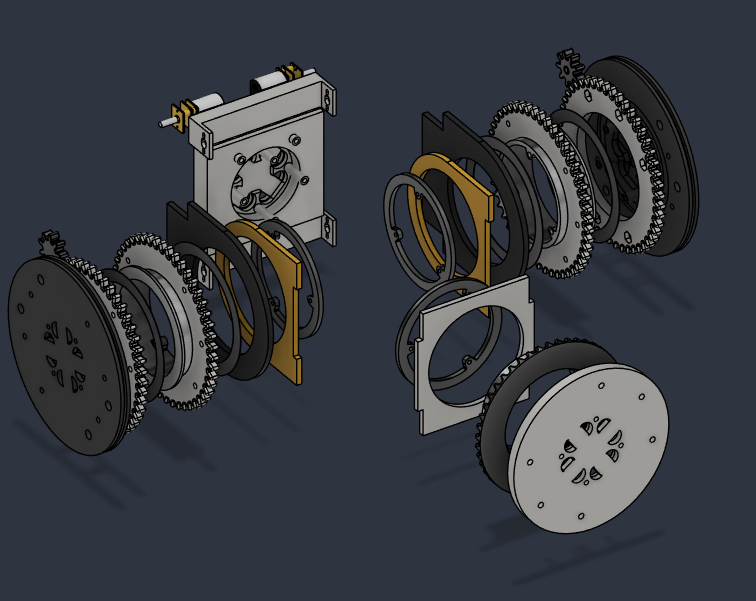
\includegraphics[width=0.6\textwidth]{../image/exploded_view.png}
	\caption{Exploded view of the module.}
	\label{fig:exploded-view}
\end{figure}

\begin{figure}[!htbp]
	\centering
	\begin{subfigure}[b]{0.40\textwidth}
		\centering
		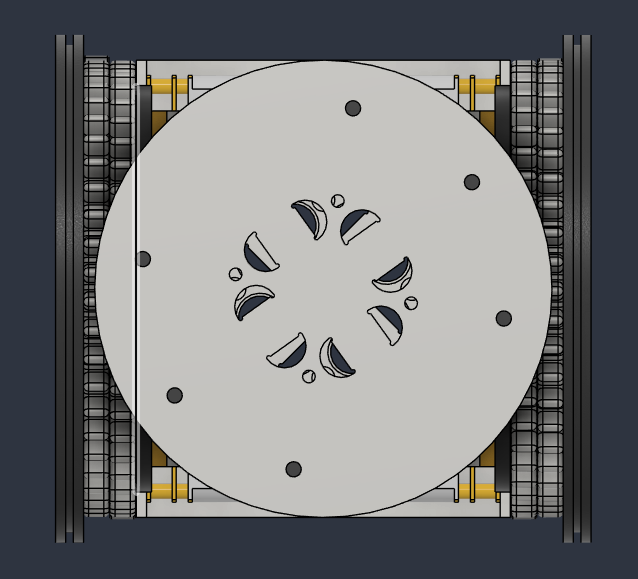
\includegraphics[width=\linewidth]{../image/front.png}
		\caption{Front view.}
		\label{fig:cad-front}
	\end{subfigure}
	\hfill
	\begin{subfigure}[b]{0.40\textwidth}
		\centering
		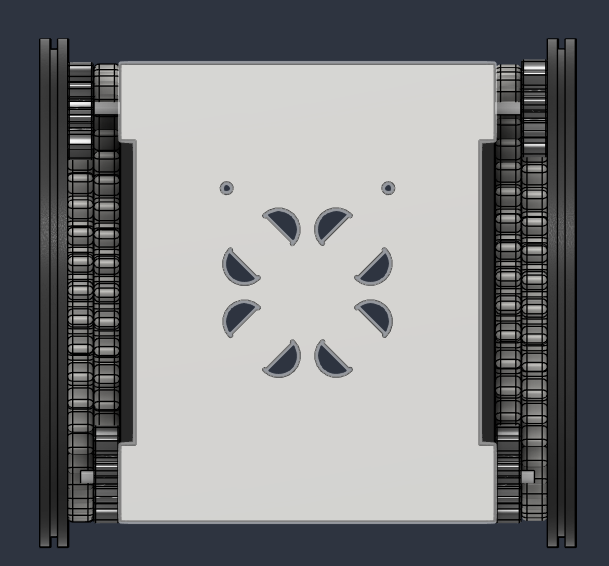
\includegraphics[width=\linewidth]{../image/rear.png}
		\caption{Rear view.}
		\label{fig:cad-rear}
	\end{subfigure}
	\par\vspace{6pt}
	\begin{subfigure}[b]{0.40\textwidth}
		\centering
		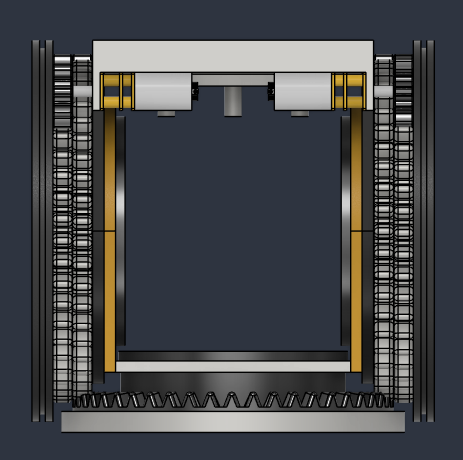
\includegraphics[width=\linewidth]{../image/top.png}
		\caption{Top view.}
		\label{fig:cad-top}
	\end{subfigure}
	\hfill
	\begin{subfigure}[b]{0.40\textwidth}
		\centering
		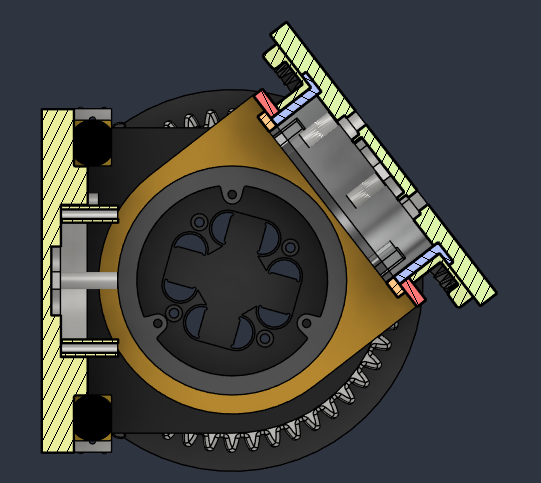
\includegraphics[width=\linewidth]{../image/tilt.png}
		\caption{Tilted sectional view.}
		\label{fig:cad-tilt}
	\end{subfigure}
	\caption{Module CAD views.}
	\label{fig:cad-views}
\end{figure}

% ----------------------------------------------------------------
\subsection{Assembled Prototype}
\label{sec:assembled-prototype}

Figures~\ref{fig:real-views} and~\ref{fig:real-views-2} show the physically
assembled module, with printed wheels, pan and tilt faces, spur and crown gears,
and N20 motors mounted in the frame.

\begin{figure}[!htbp]
	\centering
	\begin{subfigure}[t]{0.40\textwidth}
		\centering
		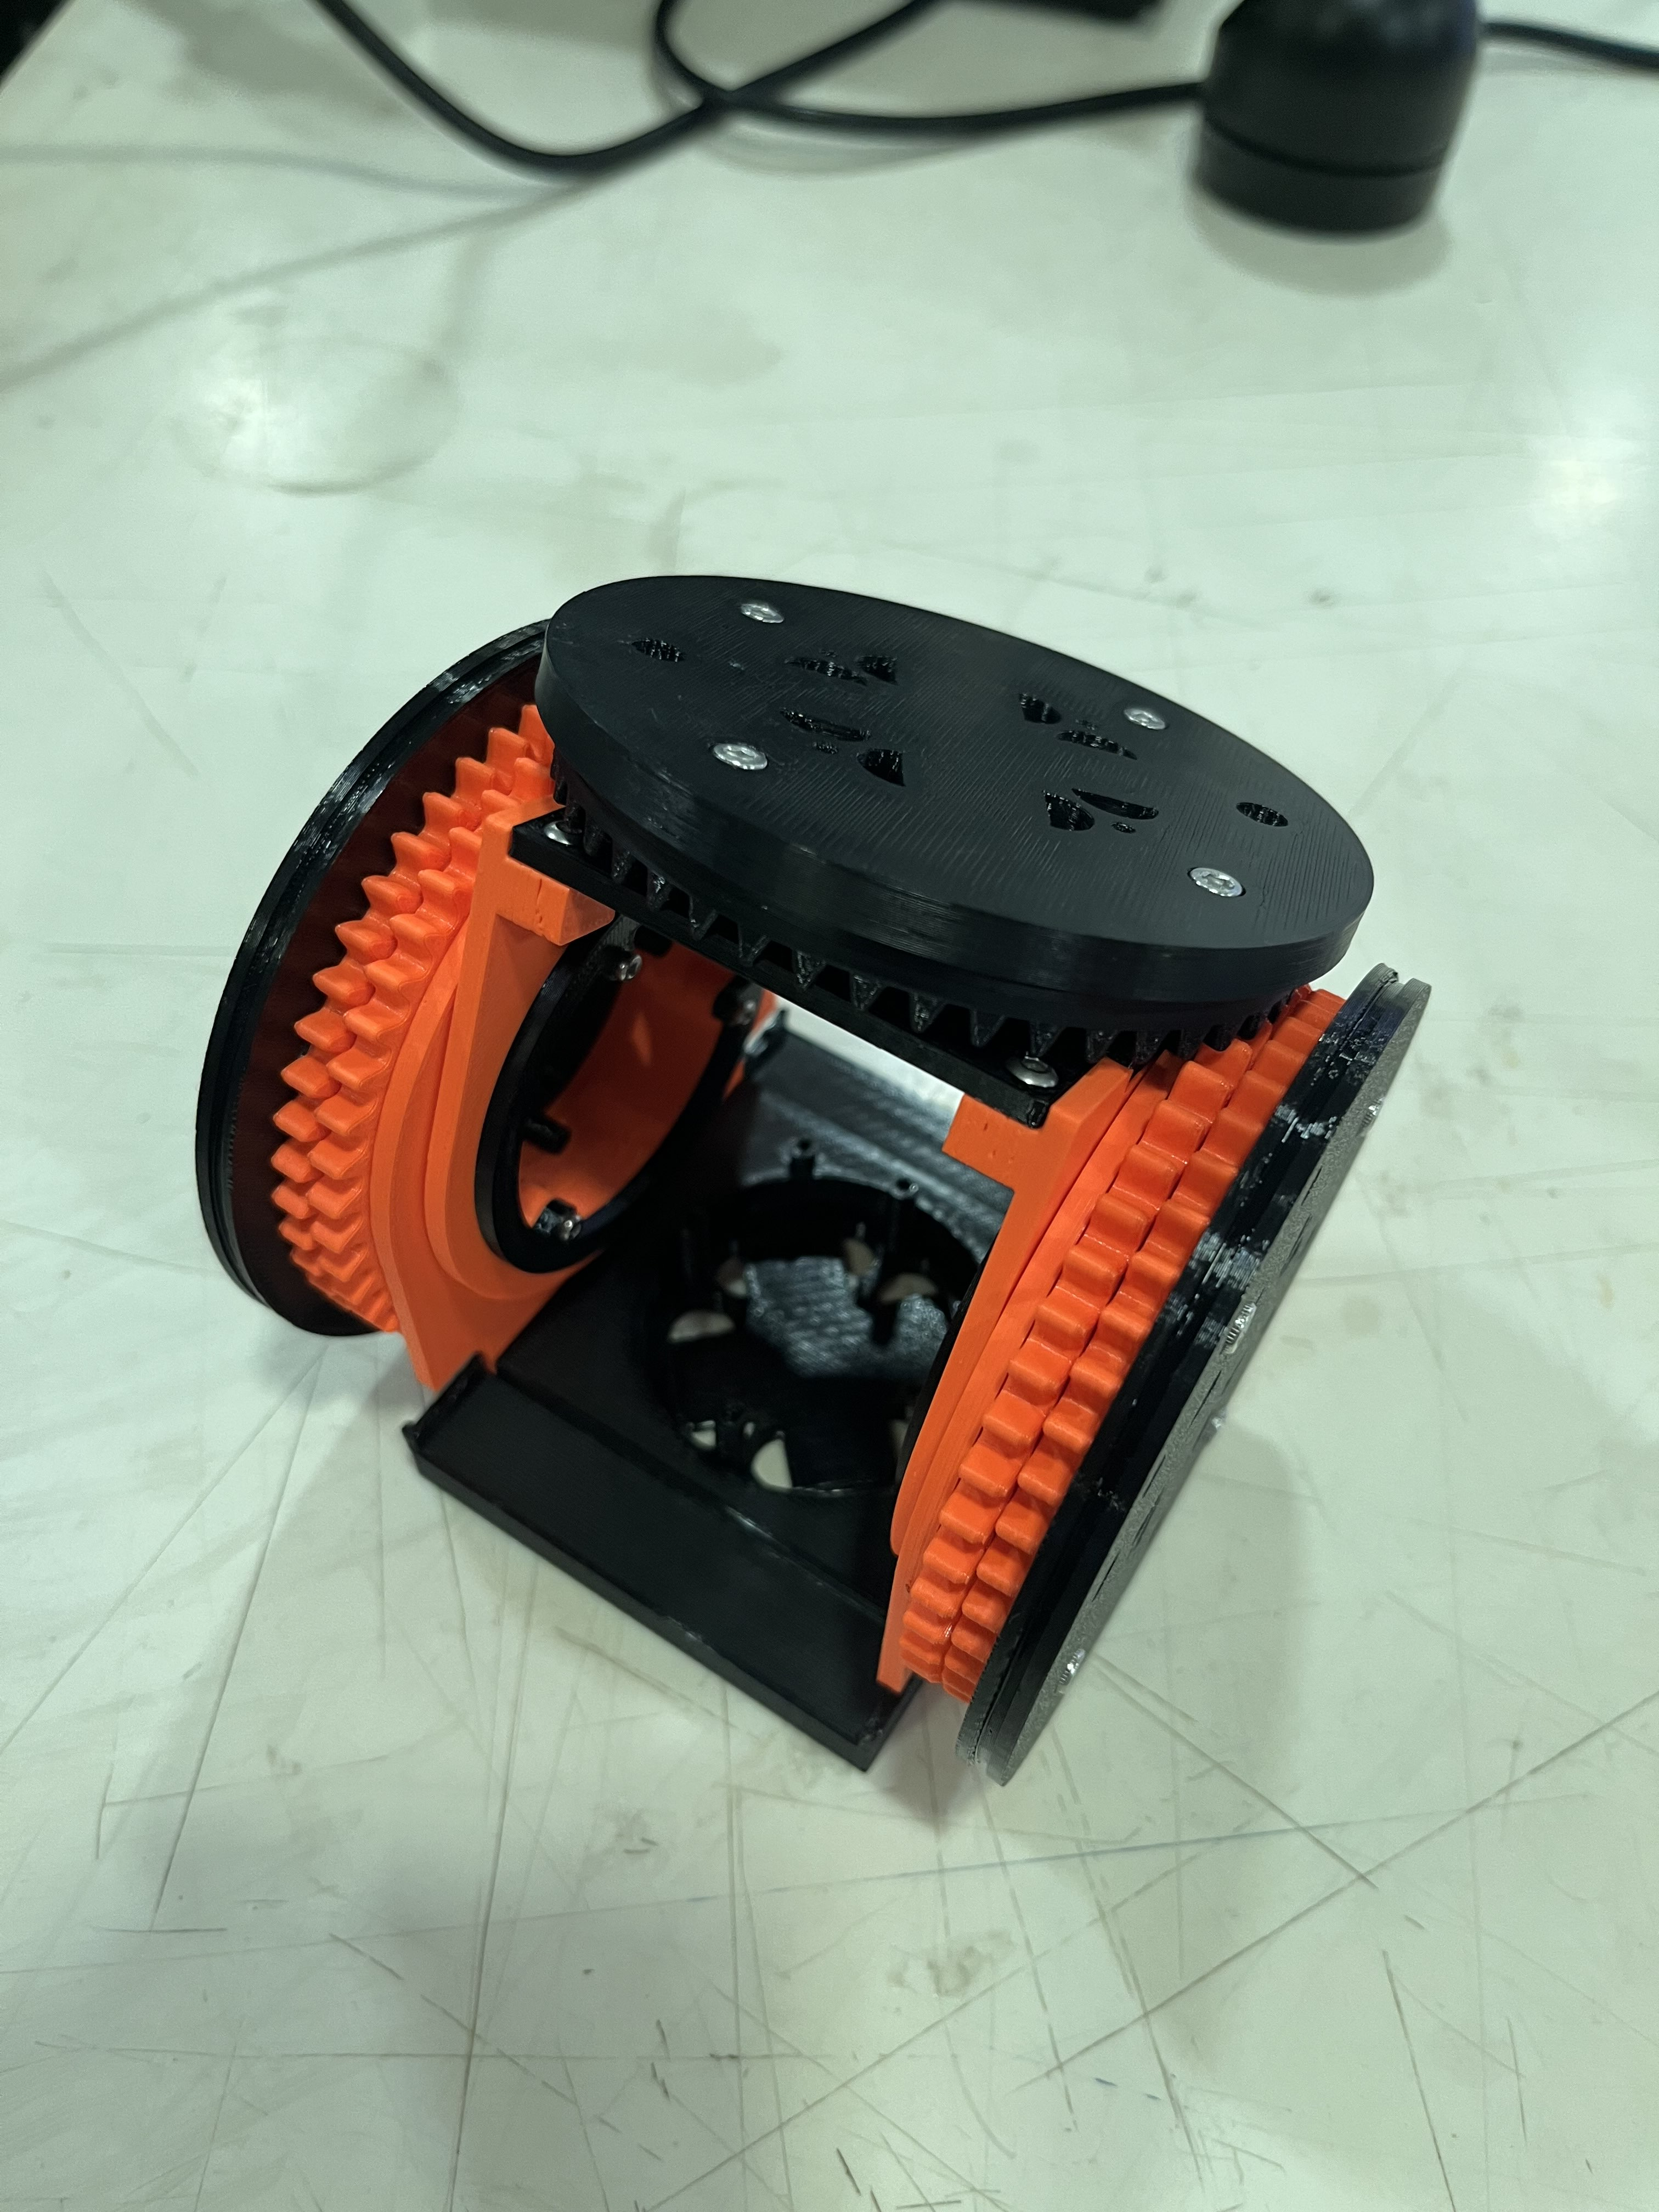
\includegraphics[width=\linewidth]{../image/assembled_iso_view.jpg}
		\caption{Oblique view of the pan face and crown gear.}
		\label{fig:real-iso}
	\end{subfigure}
	\hfill
	\begin{subfigure}[t]{0.40\textwidth}
		\centering
		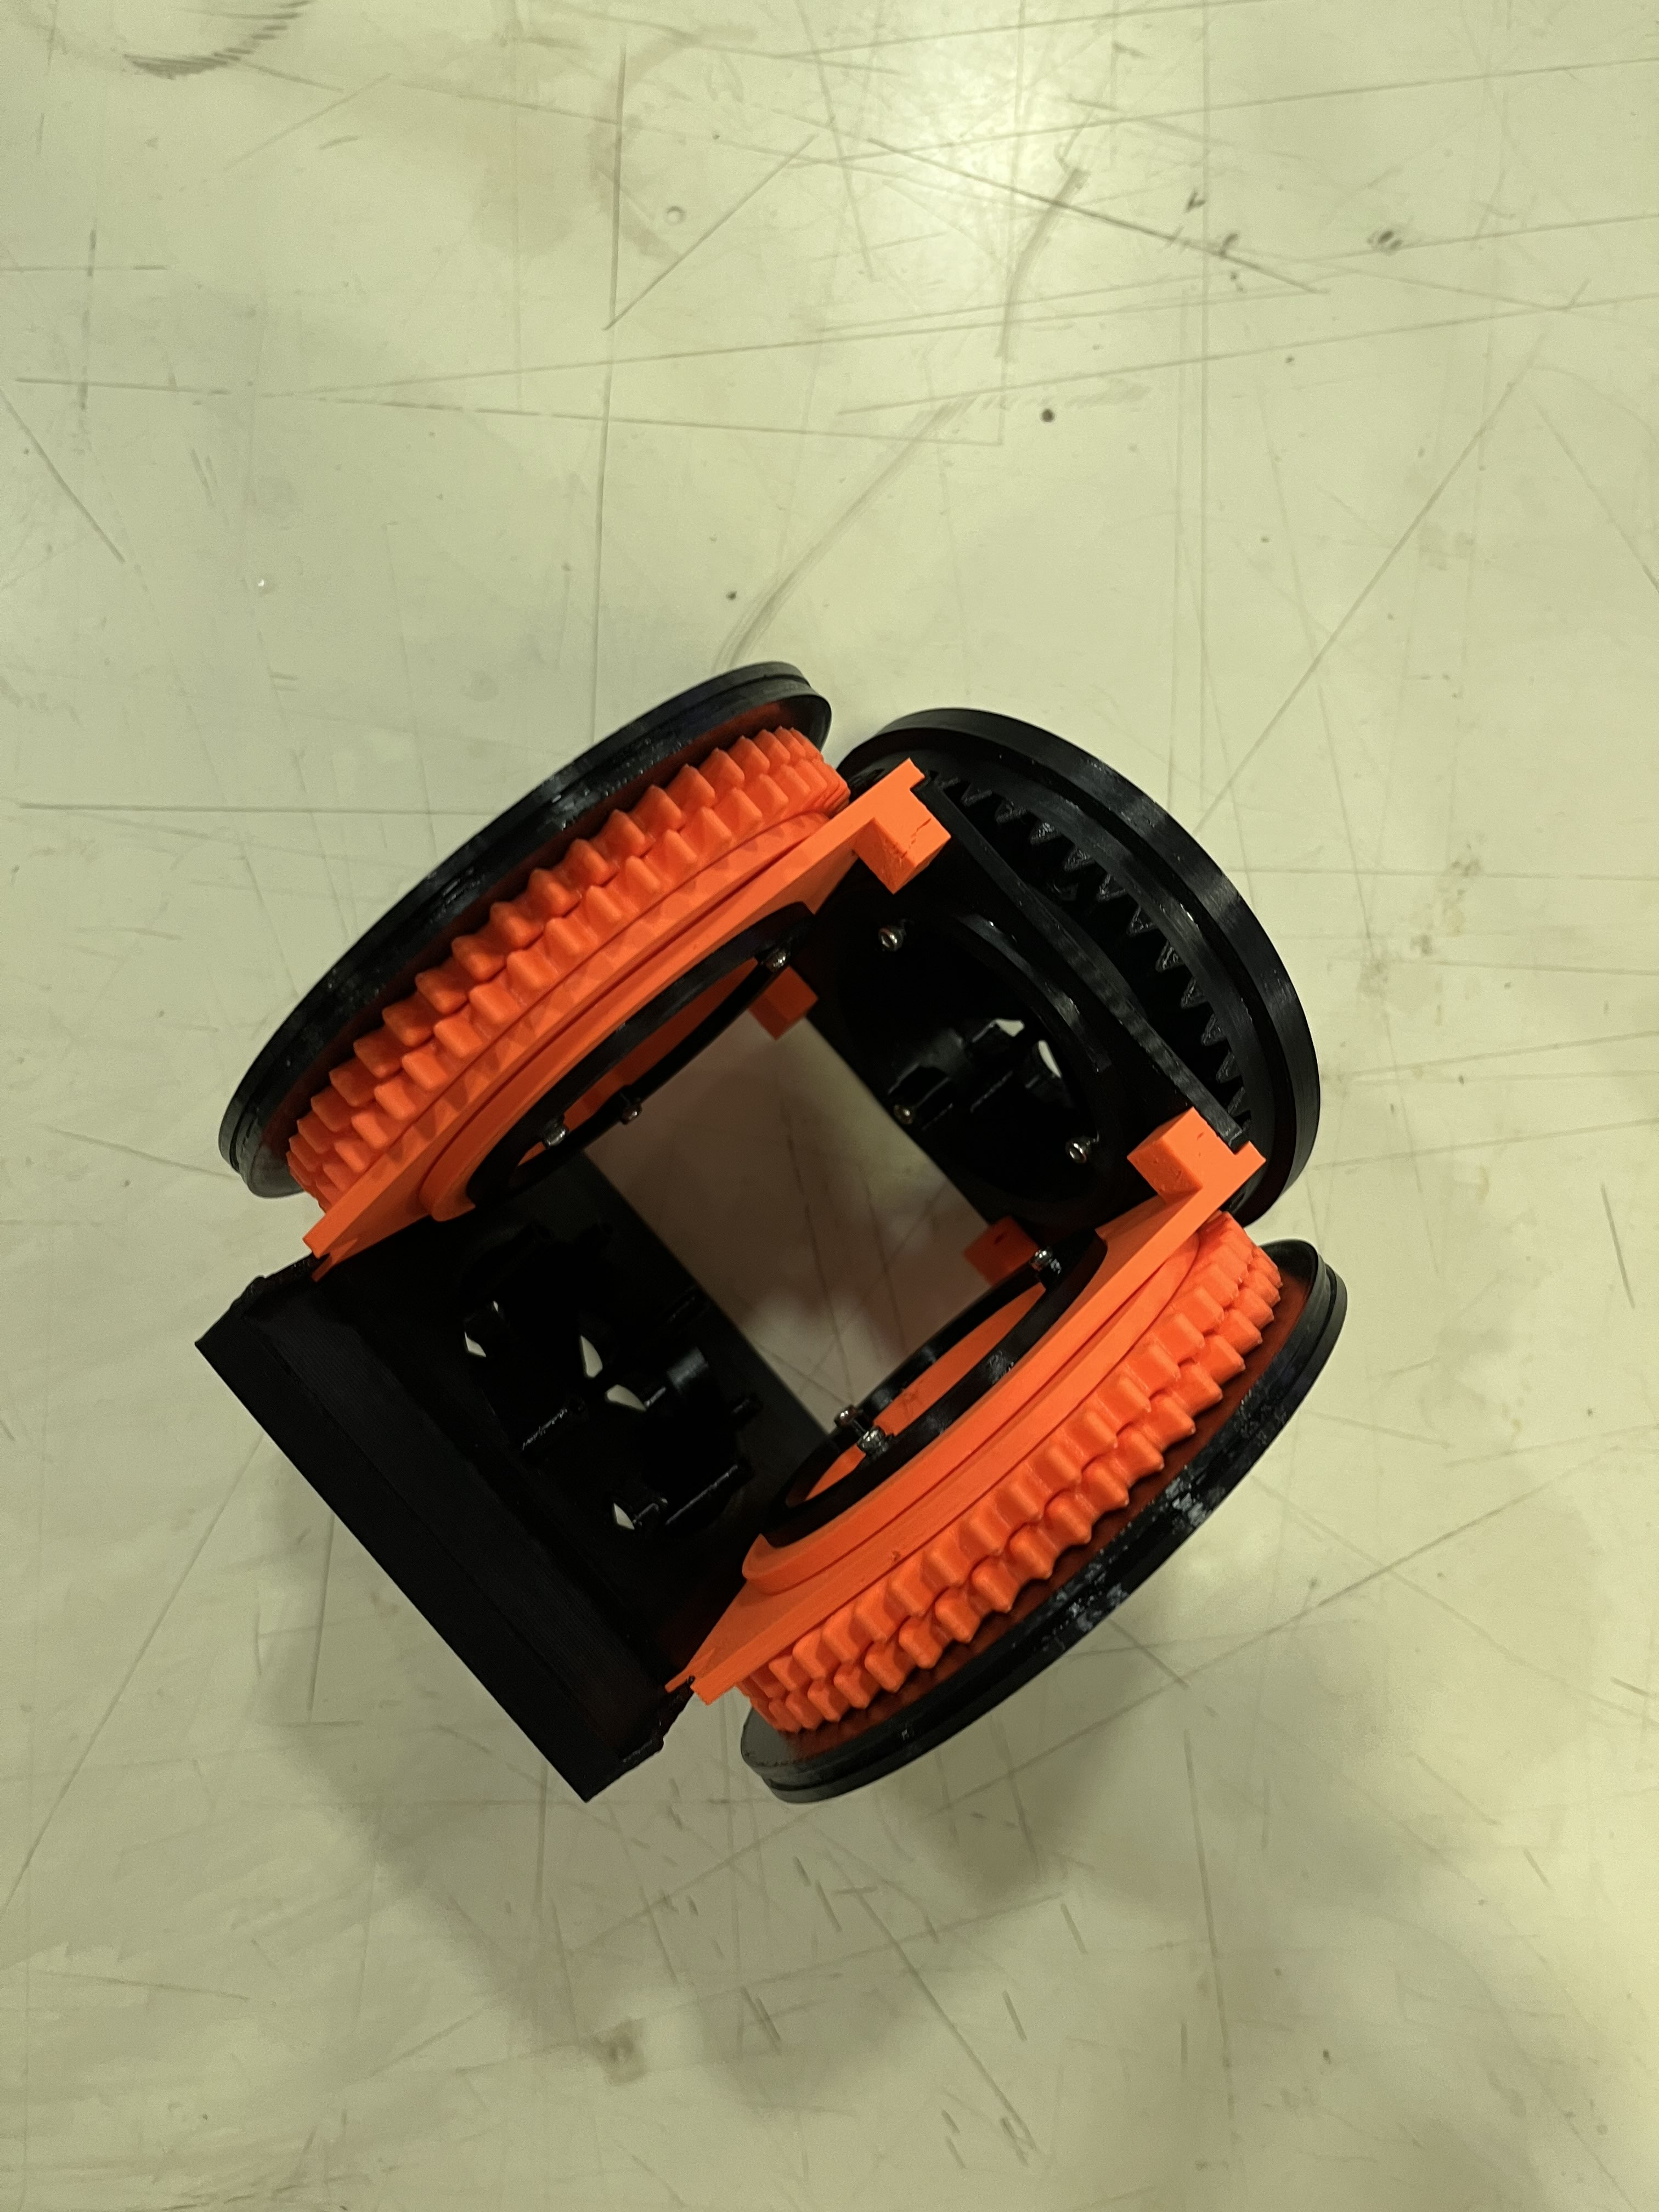
\includegraphics[width=\linewidth]{../image/assembled_top_view.jpg}
		\caption{Top view of wheels, spur gears, and frame.}
		\label{fig:real-top}
	\end{subfigure}
	\par\vspace{6pt}
	\begin{subfigure}[t]{0.40\textwidth}
		\centering
		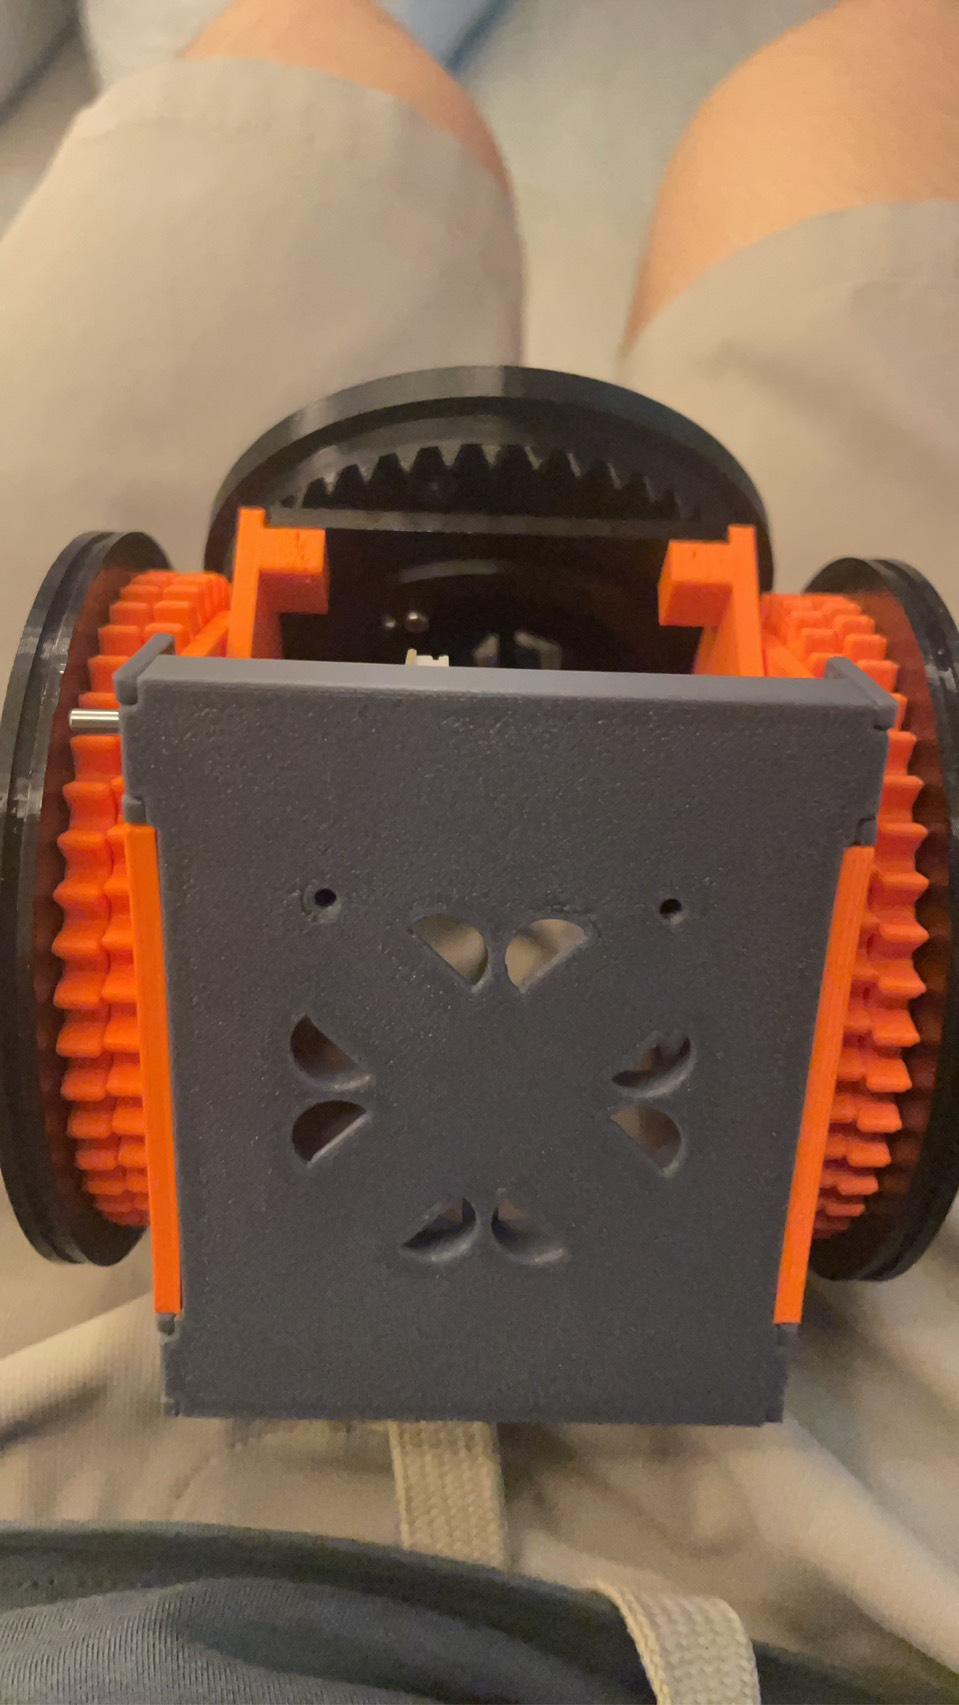
\includegraphics[width=\linewidth]{../image/assembled_tilt_face.jpg}
		\caption{Tilt face with EP-magnet openings.}
		\label{fig:real-tilt}
	\end{subfigure}
	\hfill
	\begin{subfigure}[t]{0.40\textwidth}
		\centering
		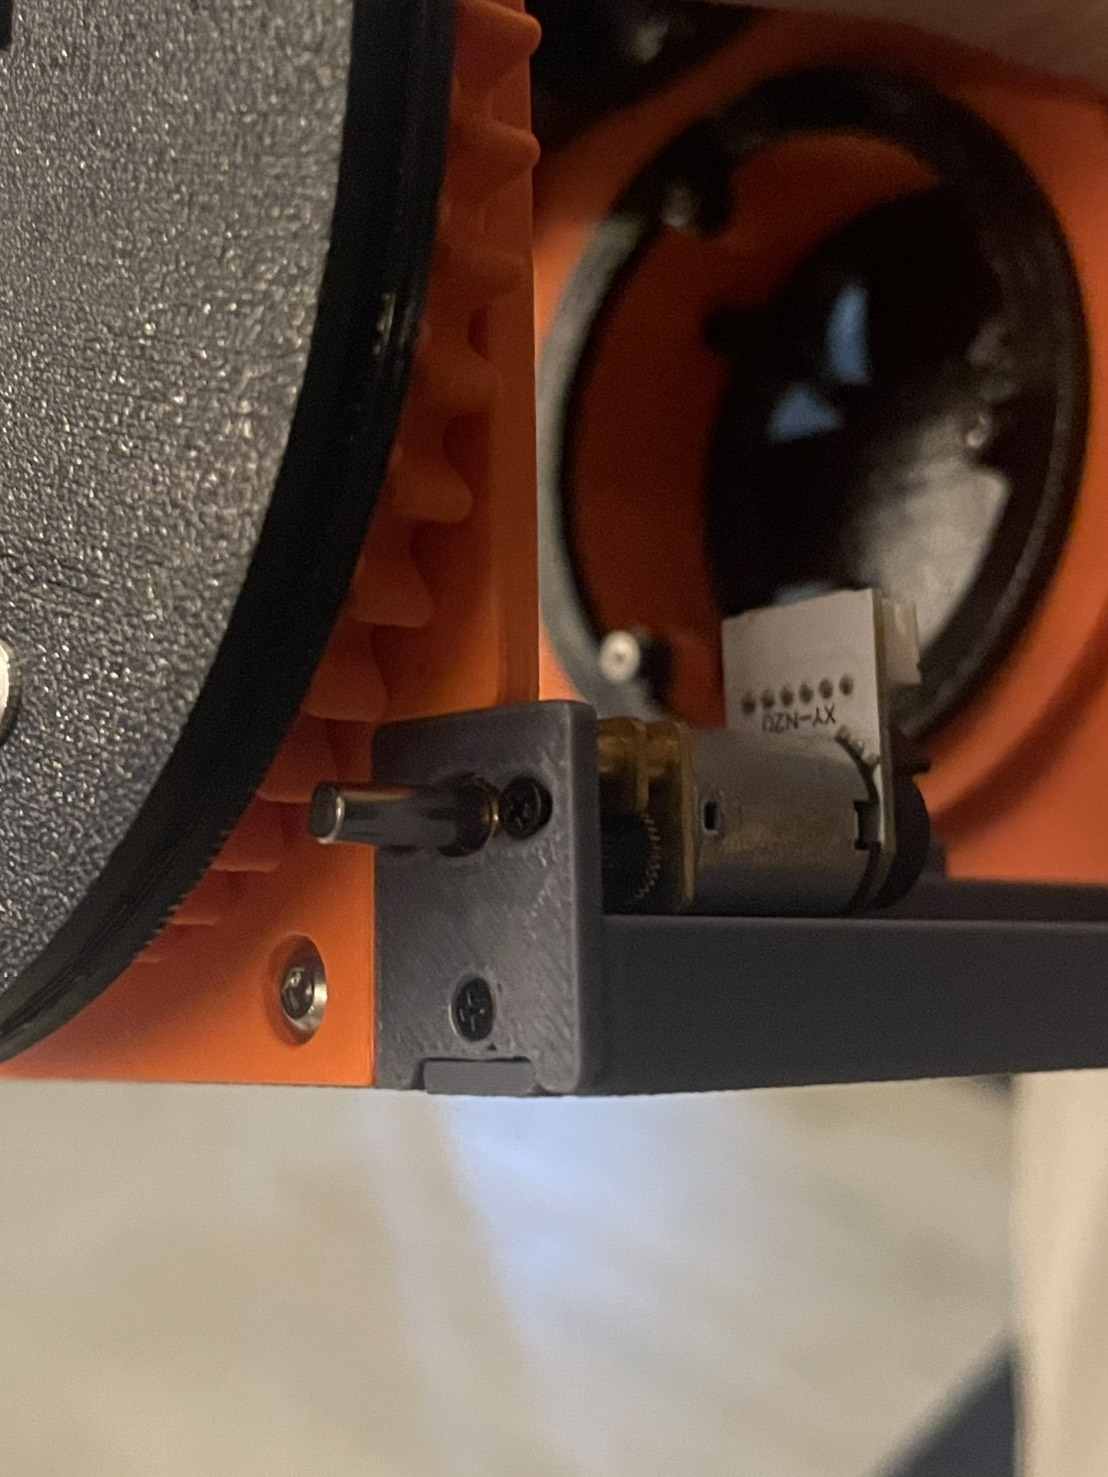
\includegraphics[width=\linewidth]{../image/assembled_motor_mount.jpg}
		\caption{N20 gearmotor in its printed mount.}
		\label{fig:real-motor}
	\end{subfigure}
	\caption{Assembled prototype (1/2).}
	\label{fig:real-views}
\end{figure}

\begin{figure}[!htbp]
	\centering
	\begin{subfigure}[t]{0.40\textwidth}
		\centering
		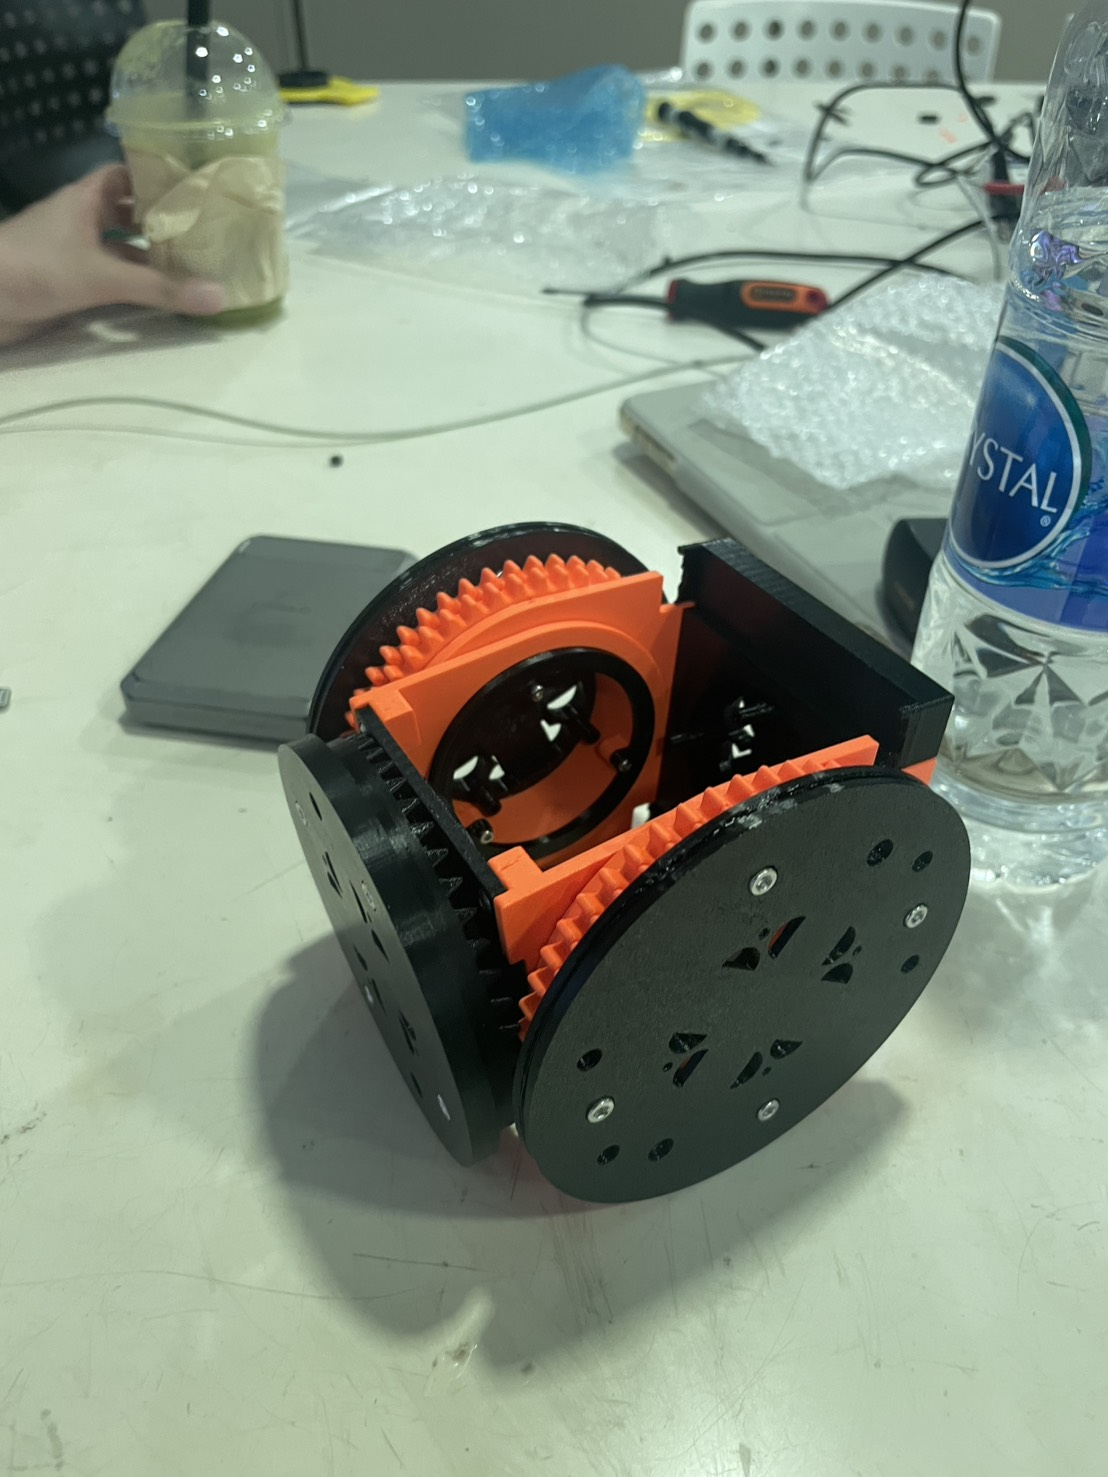
\includegraphics[width=\linewidth]{../image/assembled_workbench.jpg}
		\caption{Module on the workbench.}
		\label{fig:real-bench}
	\end{subfigure}
	\hfill
	\begin{subfigure}[t]{0.40\textwidth}
		\centering
		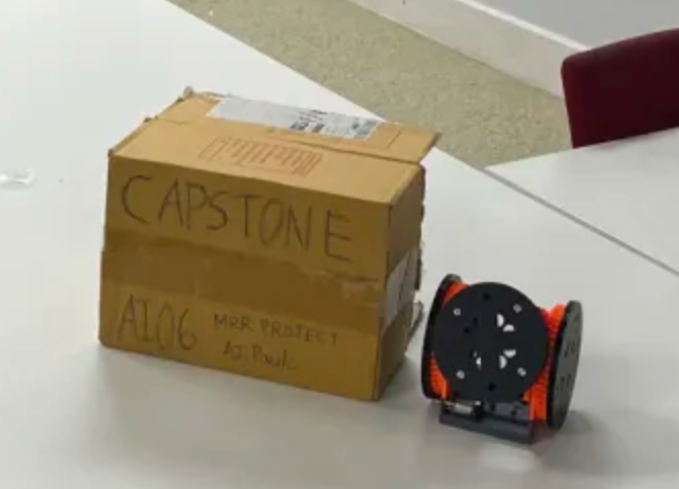
\includegraphics[width=\linewidth]{../image/assembled_size_reference.png}
		\caption{Module next to a cardboard box for scale.}
		\label{fig:real-size}
	\end{subfigure}
	\caption{Assembled prototype (2/2).}
	\label{fig:real-views-2}
\end{figure}

% ----------------------------------------------------------------
\subsection{Gear Train Design}
\label{sec:gear-design}

\begin{figure}[!htbp]
	\centering
	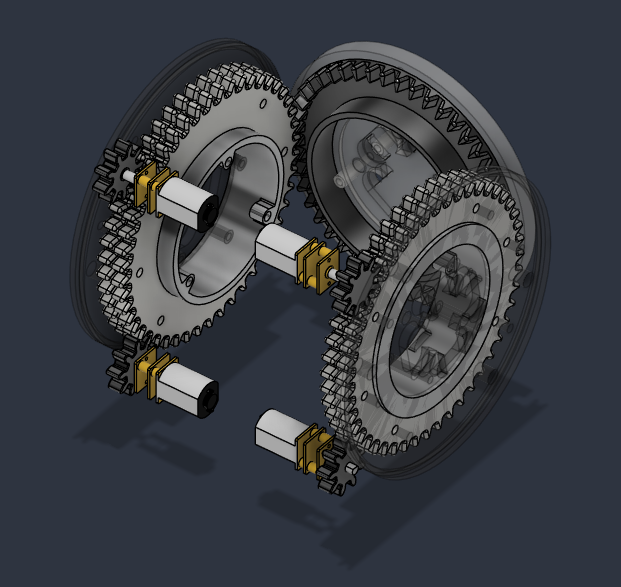
\includegraphics[width=0.6\textwidth]{../image/GearCAD.png}
	\caption{CAD view of the gear train and motor arrangement (48T spur gears, 9T pinions, 46T crown gear).}
	\label{fig:cad-gear-train}
\end{figure}

\subsubsection{SMORES-EP Reference Baseline}

The original SMORES-EP gear train was reverse-engineered from published data
(Table~\ref{tab:smores-ref}). This gives module $m = 1.4$, a spur pitch
diameter of $1.4 \times 48 = \SI{67.2}{mm}$ (OD $= 1.4 \times 50 = \SI{70}{mm}$),
and a stage ratio of $48/9 \approx 5.33$.

\begin{table}[H]
	\centering
	\caption{Reconstructed SMORES-EP reference parameters.}
	\label{tab:smores-ref}
	\begin{tabular}{ll}
		\toprule
		\textbf{Parameter} & \textbf{SMORES-EP} \\
		\midrule
		Module envelope & $80 \times 80 \times 80$\,mm \\
		Module $m$      & \num{1.4} \\
		Spur gear       & 48 teeth (PD \SI{67.2}{mm}, OD \SI{70}{mm}) \\
		Pinion          & 9 teeth \\
		Stage ratio     & $48/9 \approx 5.33{:}1$ \\
		Crown gear      & Same part as spur, used at \SI{90}{\degree} \\
		Gearbox         & 298:1 \\
		\bottomrule
	\end{tabular}
\end{table}

\subsubsection{Spur Gear and Pinion}

After wall thickness, bearing seats, and running clearance, the \SI{100}{mm}
envelope allows a maximum spur gear OD of \SI{90}{mm}. The final design keeps the
SMORES-EP tooth counts (48T spur, 9T pinion) and scales the module from
$m = 1.4$ to $m = 1.8$, so the spur OD is $m(z+2) = 1.8 \times 50 = \SI{90}{mm}$
and fills the available diameter exactly. The resulting spur--pinion centre
distance is $m(z_1+z_2)/2 = 1.8 \times 57 / 2 = \SI{51.3}{mm}$.

Reasons for this choice:
\begin{itemize}
	\item \textbf{Ratio preserved.} The $48/9 \approx 5.33{:}1$ stage ratio is
	      unchanged, so the gearbox selection, the SMORES-EP performance
	      benchmarks, and the control/firmware tuning all remain valid.
	\item \textbf{Direct comparability.} Using the same tooth counts as SMORES-EP
	      means the gear train differs from the reference only in scale.
	\item \textbf{Larger, stronger teeth.} At $m = 1.8$ the tooth thickness on the
	      pitch circle is $\pi m/2 \approx \SI{2.83}{mm}$, compared with
	      \SI{2.14}{mm} for $m = 1.36$. This makes the teeth stronger in FDM nylon
	      and less sensitive to print tolerances.
	\item \textbf{Adequate pinion size.} The 9T pinion has an OD of
	      $1.8 \times 11 = \SI{19.8}{mm}$, about the same as the 12T alternative
	      (\SI{19.04}{mm}), so there is still enough material around the
	      motor-shaft bore.
\end{itemize}

\textbf{Design change from the previous draft.} An earlier draft proposed a
64T/12T pair at $m = 1.36$ (same 5.33:1 ratio) to reduce pinion undercut and
raise the contact ratio. This was replaced by the 48T/9T, $m = 1.8$ pair, which
meshed and turned smoothly in print testing.

\textbf{Pinion undercut.} A 9-tooth pinion at a \SI{20}{\degree} pressure angle is
well below the theoretical minimum tooth count for no undercut
($z_{\min} = 2/\sin^2\alpha \approx 17$), so some root undercut is unavoidable.
SMORES-EP has the same undercut. It was accepted because the printed pair meshes
and runs smoothly.

\textbf{Motor-shaft D-bore.} The pinions mount on the N20 gearmotor D-shaft.
The bore was first modelled with a \SI{0.1}{mm} tolerance. To allow for
shrinkage of printed nylon holes, the D-bore tolerance has since been made
slightly larger. The revised bore has not yet been print tested.

\subsubsection{Pan/Tilt Crown Gear}

SMORES-EP reuses a spur gear as a crown gear at \SI{90}{\degree}. This design
instead uses a \textbf{true crown (face) gear} to improve load distribution
across the mesh. A first attempt at \SI{90}{mm} OD interfered with surrounding
components (motors, gearboxes, and structural frame), so the crown gear was
reduced to \SI{84}{mm} OD with 46 teeth and $m = 1.75$ (pitch diameter
\SI{80.5}{mm}).

\textbf{Tooth proportions.} The crown addendum is the standard
$h_a = m = \SI{1.75}{mm}$. The dedendum does \emph{not} use the standard
$h_f = 1.25m = \SI{2.1875}{mm}$; it is set to \SI{2.15}{mm} instead. With the
\SI{1.8}{mm} addendum of the mating spur gear, this leaves a root clearance of
\SI{0.35}{mm}.

\textbf{Module mismatch.} The spur gears ($m = 1.8$) and the crown gear
($m = 1.75$) have different modules. This is an accepted compromise, because the
spur diameter, crown diameter, and tooth counts are all fixed by packaging and
ratio constraints. The mismatch is small (about 2.8\,\%). The circular pitch is
$\pi m = \SI{5.65}{mm}$ for the spur gear and \SI{5.50}{mm} for the crown gear,
a difference of about \SI{0.16}{mm} per tooth, which is the same order as the
\SI{0.2}{mm} backlash allowance. Print testing confirmed that the spur--crown
mesh turns smoothly despite the mismatch.

\subsubsection{Final Gear Parameters}

\begin{table}[H]
	\centering\small
	\caption{Final gear train parameters.}
	\label{tab:final-params}
	\begin{tabular}{lllllp{4.2cm}}
		\toprule
		\textbf{Component} & \textbf{Teeth} & \textbf{Module} & \textbf{PD} & \textbf{OD} & \textbf{Notes} \\
		\midrule
		Spur gear ($\times$4) & 48 & \num{1.8} & \SI{86.4}{mm} & \SI{90}{mm} &
		\SI{5}{mm} face width, bolt holes in web \\
		\addlinespace
		Pinion ($\times$4) & 9 & \num{1.8} & \SI{16.2}{mm} & \SI{19.8}{mm} &
		D-bore tolerance slightly enlarged (not yet print tested); through-bore
		(pan/tilt) or blind (wheel) \\
		\addlinespace
		Crown gear & 46 & \num{1.75} & \SI{80.5}{mm} & \SI{84}{mm} &
		True face gear; $h_a = \SI{1.75}{mm}$, $h_f = \SI{2.15}{mm}$ \\
		\bottomrule
	\end{tabular}
\end{table}

Common to all gears: \SI{20}{\degree} pressure angle, \SI{0.2}{mm} backlash, and
\SI{0.3}{mm} root fillet. The backlash and fillet are deliberate manufacturing
allowances. The spur--pinion centre distance is \SI{51.3}{mm}. All gears were
generated with the Fusion~360 spur gear tool and 3D-printed in nylon.

\subsubsection{Drivetrain Architecture}

Four motors each drive a 9T pinion meshing with a 48T spur gear:
\begin{itemize}
	\item \textbf{Outer two:} each drives a wheel (differential-drive locomotion).
	\item \textbf{Inner two:} both mesh with a single crown gear, which works as a
	      differential:
	      \begin{itemize}
	      	\item Both spur gears turning the \emph{same} direction about their
	      	      shared axis $\rightarrow$ the crown gear does not spin; the whole
	      	      crown assembly rotates about the shared axis (\textbf{tilt}).
	      	\item Spur gears turning in \emph{opposite} directions $\rightarrow$
	      	      the crown gear spins about its own axis (\textbf{pan}).
	      \end{itemize}
\end{itemize}
The crown gear must mesh symmetrically with both inner spur gears. Any
asymmetry would couple the pan and tilt motions.

\subsubsection{Status}

All gears (48T spur, 9T pinion, and 46T crown) have been printed and tested.
Both the spur--pinion and spur--crown meshes turn smoothly. The remaining step
is to print test the revised pinion D-bore on the motor shaft.

% ----------------------------------------------------------------
\subsection{Outer Wheels}

Two independently driven wheels (\SI{100}{mm} diameter) with NBR N70 O-ring tire groove (\SI{1.5}{mm} cross-section), EP-magnet docking space, and PCB mounting posts.

\begin{figure}[!htbp]
	\centering
	\begin{subfigure}[b]{0.45\textwidth}
		\centering
		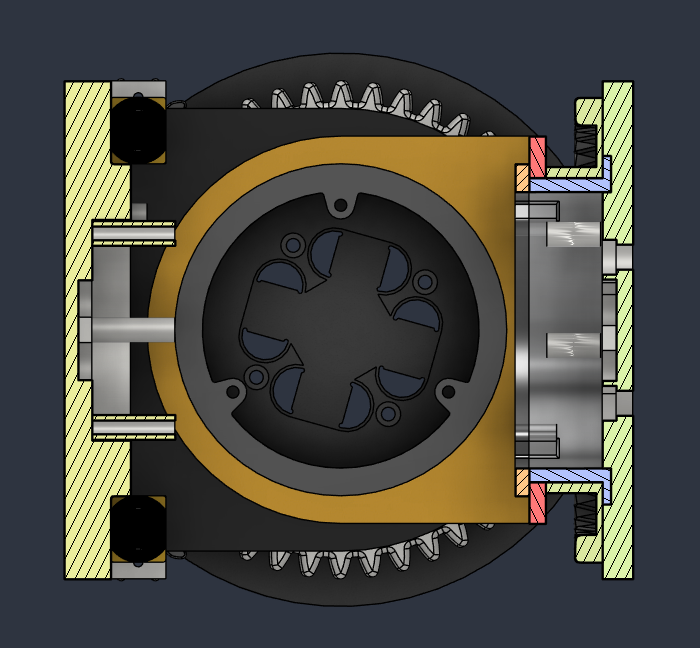
\includegraphics[width=\linewidth]{../image/inside_wheel.png}
		\caption{Interior view (wheel and drivetrain).}
		\label{fig:cad-inside-wheel}
	\end{subfigure}
	\hfill
	\begin{subfigure}[b]{0.45\textwidth}
		\centering
		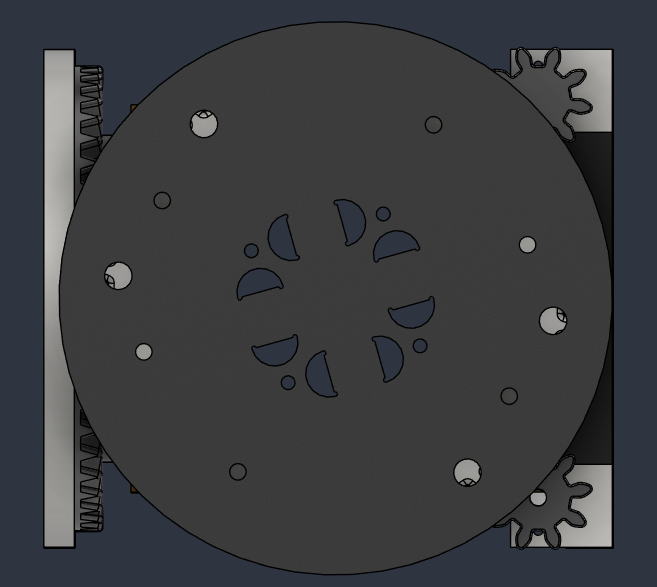
\includegraphics[width=\linewidth]{../image/outside_wheel.png}
		\caption{Exterior view (wheel and module).}
		\label{fig:cad-outside-wheel}
	\end{subfigure}
	\caption{Outer wheel CAD.}
	\label{fig:cad-wheels}
\end{figure}

\subsection{Pan Face}

\SI{90}{mm} diameter, no O-ring groove. Includes EP-magnet docking space.

\subsection{Tilt Face}

Approximately $90 \times 71.6$\,mm rectangular part with EP-magnet docking space and an additional motor mount.

\subsection{Simulation Model}
\label{sec:sim-model}

The module CAD is exported from Blender (LinkForge) to URDF and refactored into xacro, then simulated in Gazebo Fortress with \texttt{ros2\_control} on ROS~2 Humble. The model serves as a digital twin for testing control algorithms before hardware is available.

\subsubsection{Kinematic Model}

The model has five links (base, two wheels, tilt body, pan face) and four actuated joints (Table~\ref{tab:sim-joints}). The exporter placed the CAD orientation of each part in the joint frames, giving rotated and inconsistent TF frames. All link frames were therefore re-aligned with the base following REP-103 ($x$ forward, $y$ left, $z$ up), and each mesh's CAD rotation was moved into its visual and collision origin. A forward-kinematics comparison at random joint configurations confirmed every mesh pose was unchanged (maximum difference \SI{1e-6}{m}). Self-collision between the module's own links is disabled.

\begin{table}[H]
	\centering
	\caption{Simulated joints and control interfaces.}
	\label{tab:sim-joints}
	\small
	\begin{tabular}{lllll}
		\toprule
		\textbf{Joint} & \textbf{Type} & \textbf{Axis} & \textbf{Command} & \textbf{Controller} \\
		\midrule
		\texttt{left\_wheel\_joint}  & continuous & $+y$ & velocity & \texttt{diff\_drive\_controller} \\
		\texttt{right\_wheel\_joint} & continuous & $+y$ & velocity & \texttt{diff\_drive\_controller} \\
		\texttt{tilt\_body\_joint}   & revolute, $\pm\SI{180}{\degree}$ & $-y$ & position & \texttt{head\_position\_controller} \\
		\texttt{pan\_face\_joint}    & continuous & $-x$ & position & \texttt{head\_position\_controller} \\
		\bottomrule
	\end{tabular}
\end{table}

The pan/tilt differential is not modelled mechanically. The simulation exposes pan and tilt directly as joints, and the mixing to the two inner motors is left to the firmware:
\begin{equation}
	\theta_A = N_t\,\theta_{\text{tilt}} + N_p\,\theta_{\text{pan}}, \qquad
	\theta_B = N_t\,\theta_{\text{tilt}} - N_p\,\theta_{\text{pan}},
\end{equation}
where $\theta_A, \theta_B$ are the inner motor angles and $N_t, N_p$ the motor-to-joint reductions of the gear train. As a consequence, the simulation does not reproduce the shared speed and torque limit when pan and tilt move together. For the first milestone, tilt and pan are held at \SI{0}{rad}.

\subsubsection{Inertial Parameters}

The exporter's inertial values were placeholders. Every link had $I_{xx} = I_{yy} = I_{zz} = m/6$, which is the inertia of a solid \SI{1}{m} cube ($I = m(a^2 + a^2)/12$ with $a = \SI{1}{m}$), regardless of shape. For parts about \SI{0.1}{m} across this overestimates inertia by roughly $100\times$, and the centres of mass were the mesh offsets rather than true centroids.

The values were therefore recomputed from the CAD meshes, assuming a uniform solid of 3D-printed nylon PA12, $\rho = \SI{1010}{kg/m^3}$. Each closed triangle mesh is decomposed into tetrahedra formed by every face $(\mathbf{a}_k, \mathbf{b}_k, \mathbf{c}_k)$ and the origin \cite{mirtich1996}:
\begin{gather}
	V_k = \tfrac{1}{6}\,\mathbf{a}_k \cdot (\mathbf{b}_k \times \mathbf{c}_k), \qquad
	m = \rho \sum_k V_k, \qquad
	\mathbf{c} = \frac{1}{\sum_k V_k} \sum_k V_k\,\frac{\mathbf{a}_k + \mathbf{b}_k + \mathbf{c}_k}{4}, \\
	C = \rho \sum_k \frac{V_k}{20} \left[ \mathbf{a}_k\mathbf{a}_k^{T} + \mathbf{b}_k\mathbf{b}_k^{T} + \mathbf{c}_k\mathbf{c}_k^{T} + \mathbf{s}_k\mathbf{s}_k^{T} \right],
	\qquad \mathbf{s}_k = \mathbf{a}_k + \mathbf{b}_k + \mathbf{c}_k, \\
	I_{cm} = \operatorname{tr}(C)\,\mathbf{E}_3 - C - m\left[ (\mathbf{c}^{T}\mathbf{c})\,\mathbf{E}_3 - \mathbf{c}\mathbf{c}^{T} \right], \qquad
	I_{\text{link}} = R\,I_{cm}\,R^{T},
\end{gather}
where the signed volumes $V_k$ cancel outside the solid, $C$ is the second-moment matrix, $\mathbf{E}_3$ is the $3 \times 3$ identity, the bracketed term is the parallel-axis shift to the centre of mass, and $R$ rotates the result into the link frame. The method is exact for a polyhedron. Implemented in \texttt{compute\_inertia.py}, it reproduced the analytic solution of an $80 \times 50 \times 30$\,mm box with \SI{0.000}{\percent} error and of a 256-facet cylinder ($r = \SI{35}{mm}$, $h = \SI{12}{mm}$) within \SI{0.02}{\percent}, the residual being faceting. Results are listed in Table~\ref{tab:sim-inertia}; the wheels give $I_{yy} \approx 2 I_{xx}$, as expected for a disc spinning about $y$.

\begin{table}[H]
	\centering
	\caption{Computed mass properties (solid nylon PA12, inertia about the centre of mass).}
	\label{tab:sim-inertia}
	\begin{tabular}{lrrrrr}
		\toprule
		\textbf{Link} & \textbf{Volume (cm$^3$)} & \textbf{Mass (g)} &
		\textbf{$I_{xx}$ (kg\,m$^2$)} & \textbf{$I_{yy}$ (kg\,m$^2$)} & \textbf{$I_{zz}$ (kg\,m$^2$)} \\
		\midrule
		Base        & 139.95 & 141.3 & \num{2.51e-4} & \num{2.05e-4} & \num{2.57e-4} \\
		Left wheel  &  51.15 &  51.7 & \num{3.55e-5} & \num{7.00e-5} & \num{3.55e-5} \\
		Right wheel &  51.15 &  51.7 & \num{3.57e-5} & \num{7.00e-5} & \num{3.53e-5} \\
		Tilt body   &  28.39 &  28.7 & \num{3.46e-5} & \num{2.82e-5} & \num{3.33e-5} \\
		Pan face    &  37.11 &  37.5 & \num{4.36e-5} & \num{2.21e-5} & \num{2.22e-5} \\
		\bottomrule
	\end{tabular}
\end{table}

The main remaining uncertainty is in the inputs, not the method: material density, partial infill if the parts are printed by FDM, and components absent from the mesh (motors, battery, PCBs), which make the base too light. Measured part masses will replace the density estimate once parts are printed; the script accepts them directly and rescales the inertia.

\subsubsection{Multi-Module Simulation}

$N$ identical modules are spawned (default three), each in its own namespace (\texttt{module\_1}, \ldots) with its own controller manager, controllers and TF frame prefix, so modules can be commanded independently. The wheels use a differential-drive controller (wheel separation \SI{96.65}{mm}, radius \SI{50}{mm}, both measured from the meshes) driven by velocity commands $(v, \omega)$.

The first milestone localises modules with AprilTags. To test algorithms before the vision pipeline exists, each module's exact pose is taken from the physics engine and published as \texttt{/module\_i/ground\_truth/odom}. A separate package, \texttt{msrr\_control}, reads these poses and commands all modules from one node. It is limited to the real top speed of \SI{0.049}{m/s} (\SI{50}{rpm} motor output through the \num{5.33}:1 wheel gear). The AprilTag estimate will later replace the ground-truth topic without changing the algorithm code. A go-to-goal test with three modules reached all goals within \SI{1}{cm}.

\subsubsection{Status and Limitations}

\begin{itemize}
	\item Joint effort and velocity limits are placeholders, pending actuator characterisation.
	\item The pan/tilt motor coupling and gear backlash are not simulated.
	\item Docking is not modelled; Phase~B will use Gazebo's detachable joints to emulate the EP-Face connection.
	\item Each module is supported only by its wheels and settles with a \SIrange{4}{6}{\degree} lean; contact with the ground will be checked against the printed module.
\end{itemize}


\clearpage
% ================================================================
\section{Electronics}
\label{sec:electronics}
% ================================================================

\subsection{Phased Electronics Plan}

Electronics are built incrementally across project phases:

\begin{itemize}
  \item \textbf{Phase A-1:} COTS parts --- 2S battery, 4-channel motor driver with MCU, ESP32-C3 for Wi-Fi.
  \item \textbf{Phase A:} Custom PCBs --- power board (buck, LDO, 4$\times$ H-bridge with current sensing) and main board (STM32G474, IMU, UWB, Wi-Fi).
  \item \textbf{Phase B:} In-wheel PCB with EP-Face circuitry and IR contact-alignment, connected via slip ring.
  \item \textbf{Phase C:} RGB-D/ToF camera (Sipeed MaixSense A075V) + wheel encoder added; compute still external.
  \item \textbf{Phase D:} Raspberry Pi CM5 on custom carrier PCB moves compute onboard.
\end{itemize}

\begin{figure}[!htbp]
  \centering
  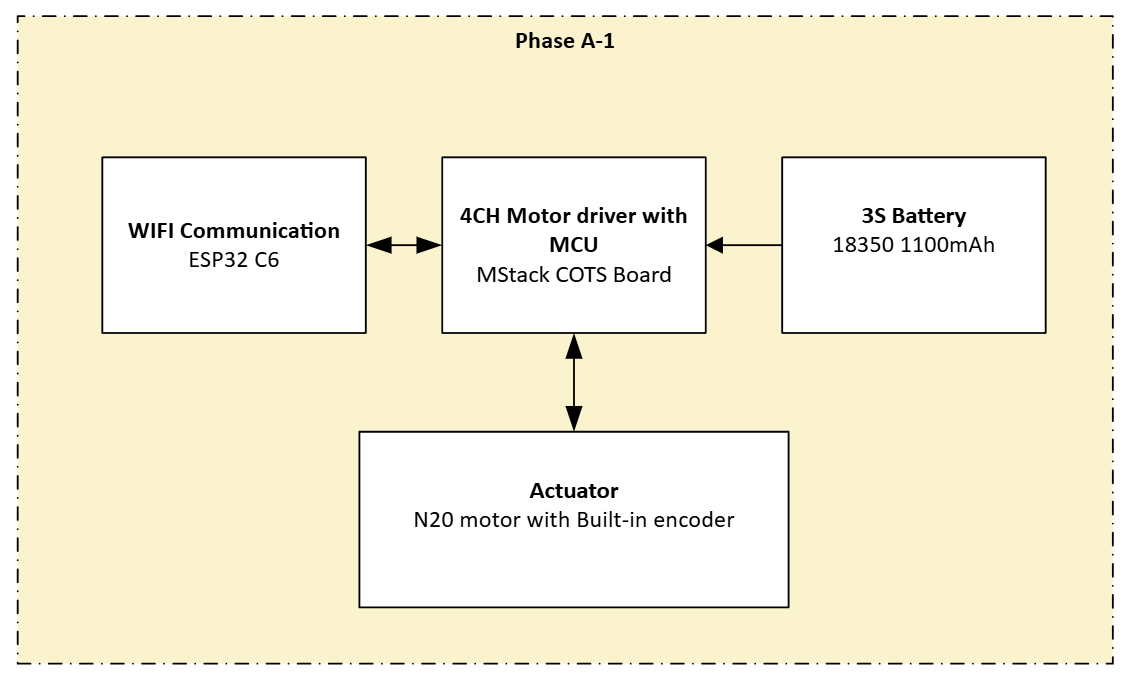
\includegraphics[width=0.78\textwidth]{../image/Phase_A_1_Diagram.png}
  \caption{Phase A-1 electronics block diagram.}
  \label{fig:phase-a1}
\end{figure}

\begin{figure}[!htbp]
	\centering
	\begin{subfigure}[b]{\textwidth}
		\centering
		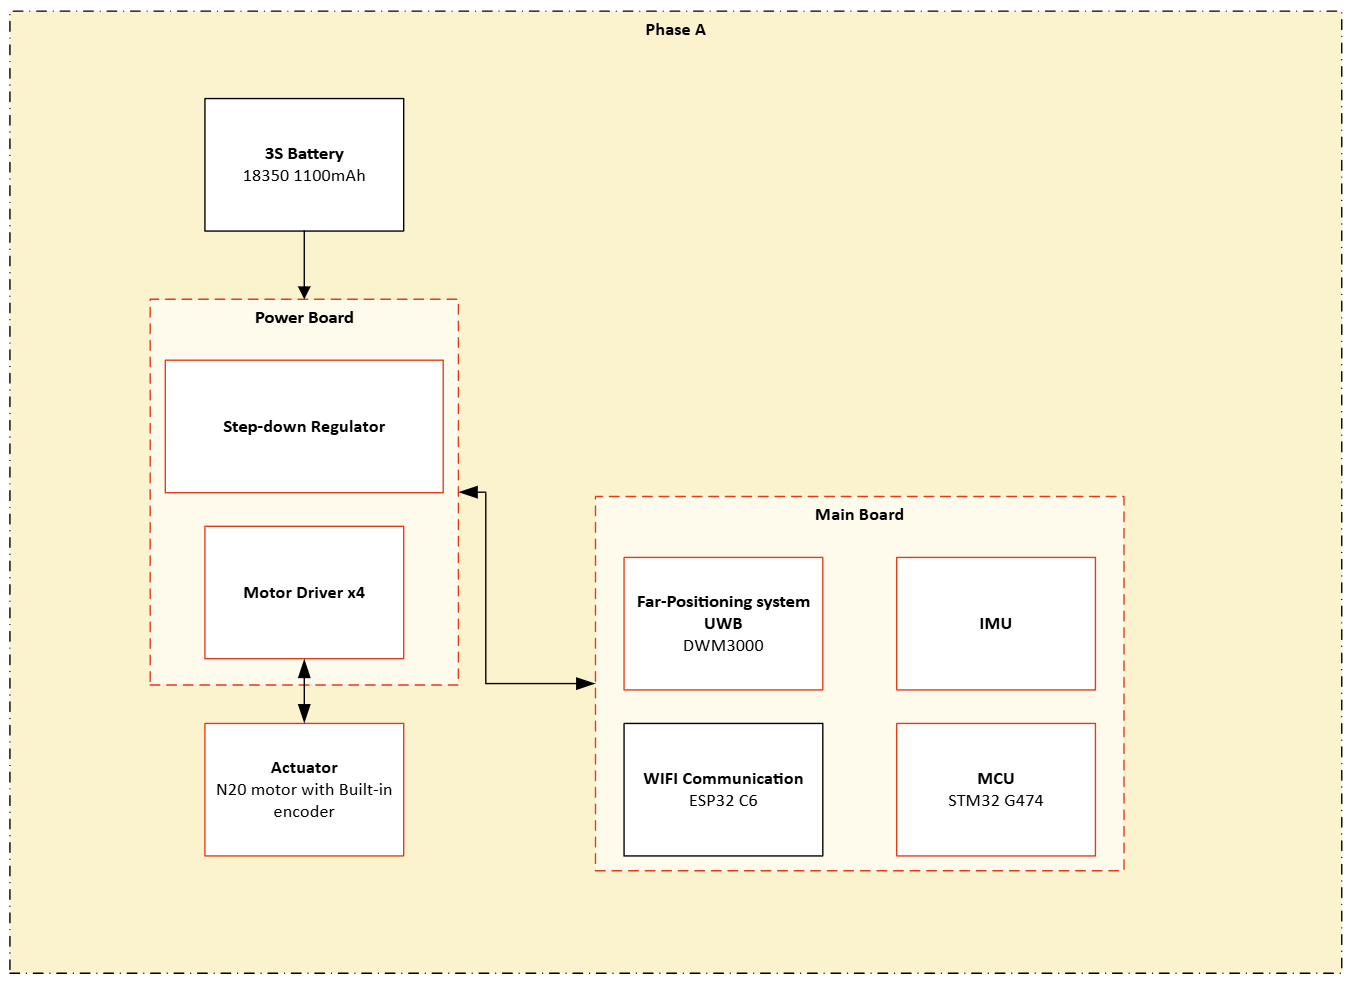
\includegraphics[width=0.78\textwidth]{../image/Phase_A_Diagram.png}
		\caption{Phase A.}
		\label{fig:phase-a}
	\end{subfigure}
	\par\vspace{8pt}
	\begin{subfigure}[b]{\textwidth}
		\centering
		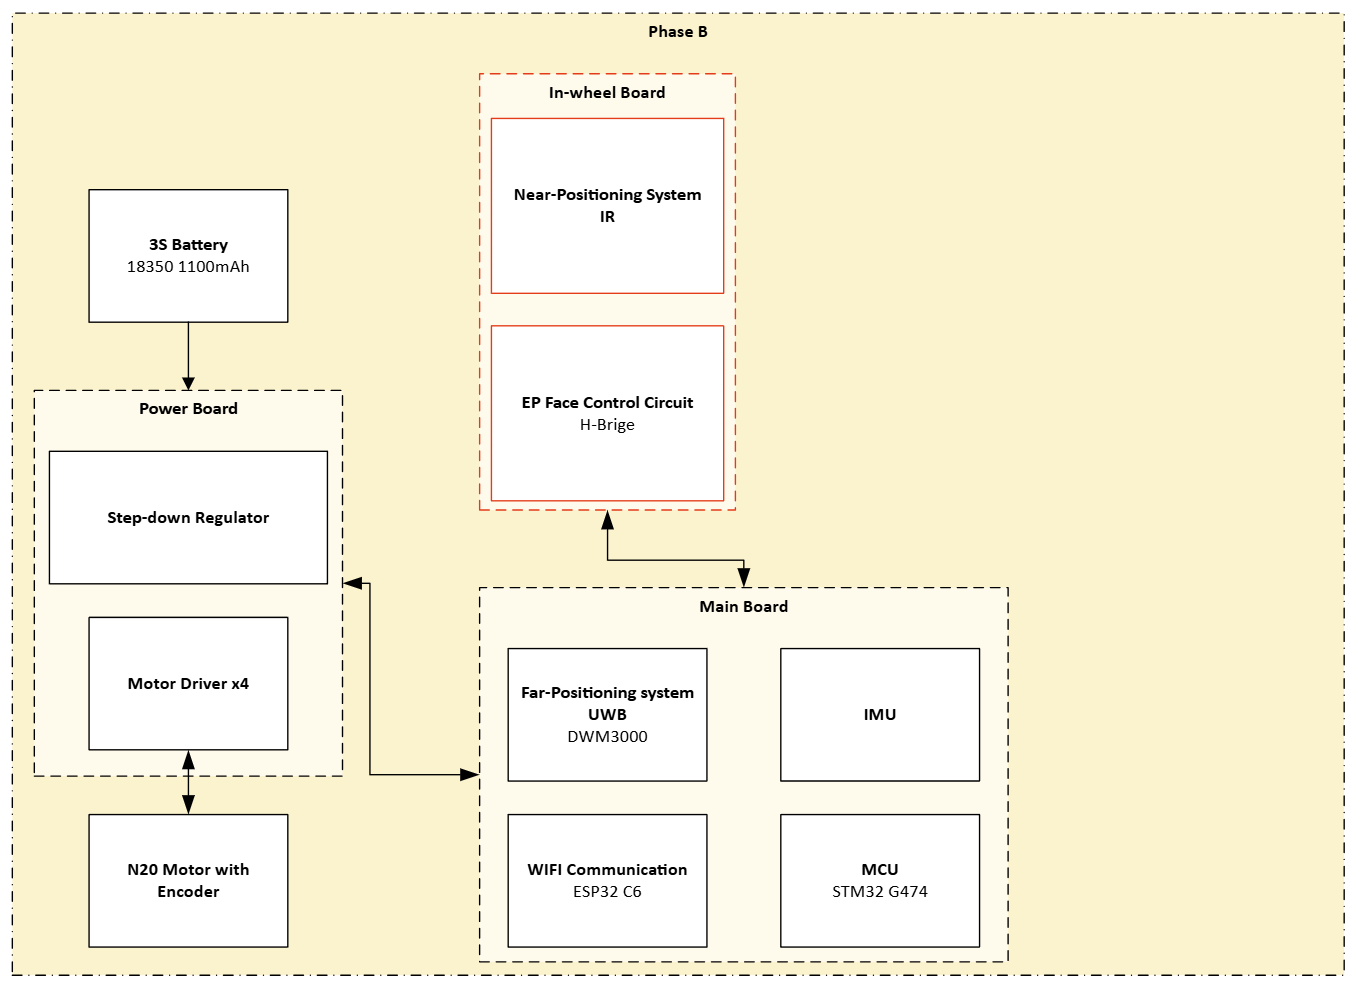
\includegraphics[width=0.78\textwidth]{../image/Phase_B_Diagram.png}
		\caption{Phase B.}
		\label{fig:phase-b}
	\end{subfigure}
	\caption{Electronics block diagrams, Phases A--B.}
	\label{fig:phase-diagrams-ab}
\end{figure}

\begin{figure}[!htbp]
	\centering
	\begin{subfigure}[b]{\textwidth}
		\centering
		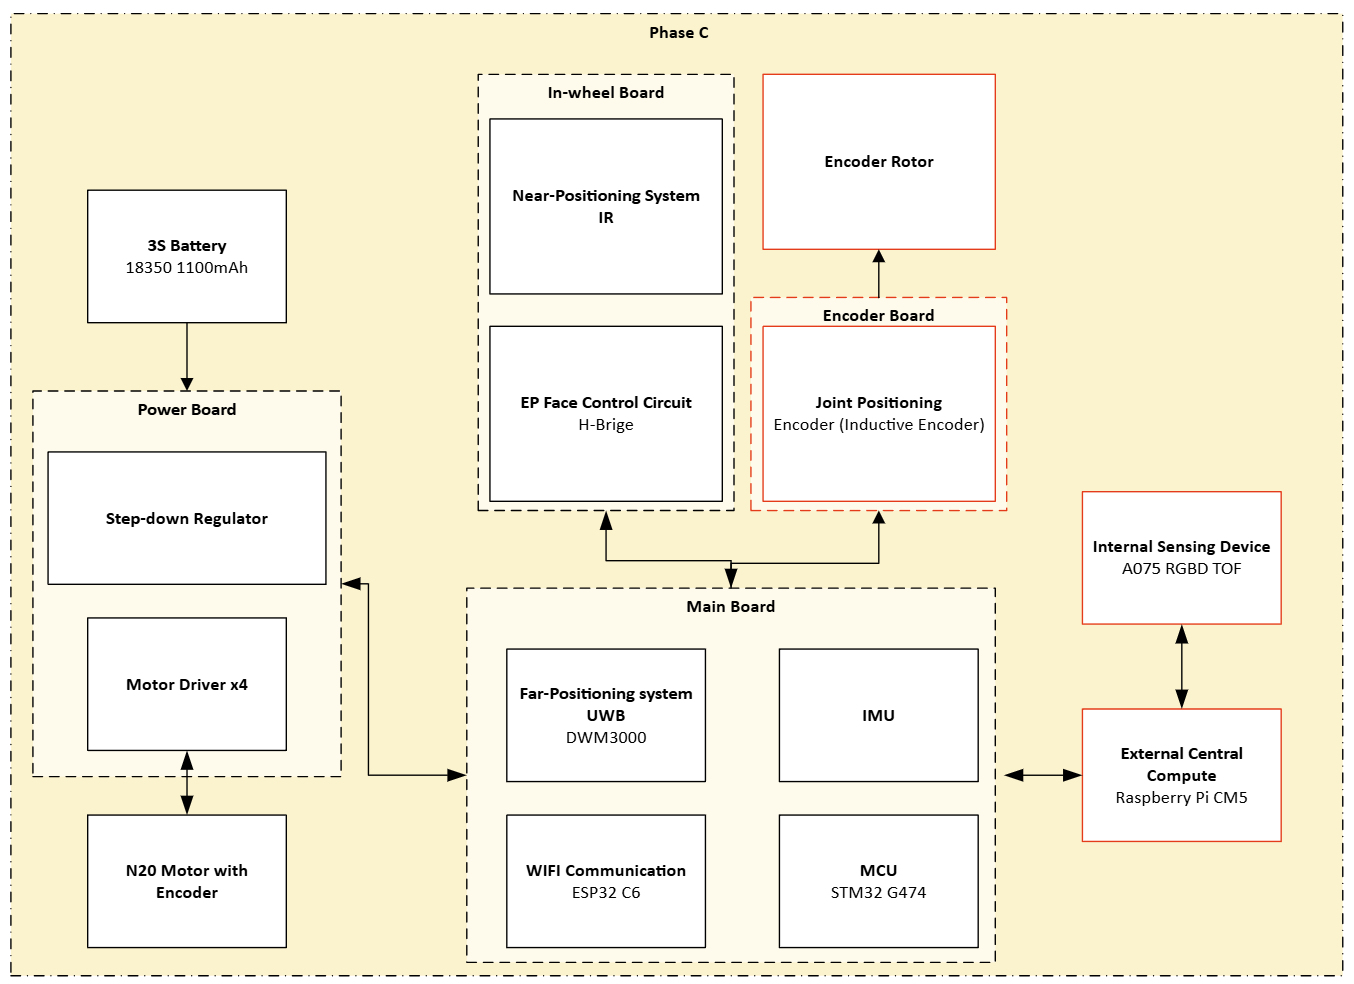
\includegraphics[width=0.78\textwidth]{../image/Phase_C_Diagram.png}
		\caption{Phase C.}
		\label{fig:phase-c}
	\end{subfigure}
	\par\vspace{8pt}
	\begin{subfigure}[b]{\textwidth}
		\centering
		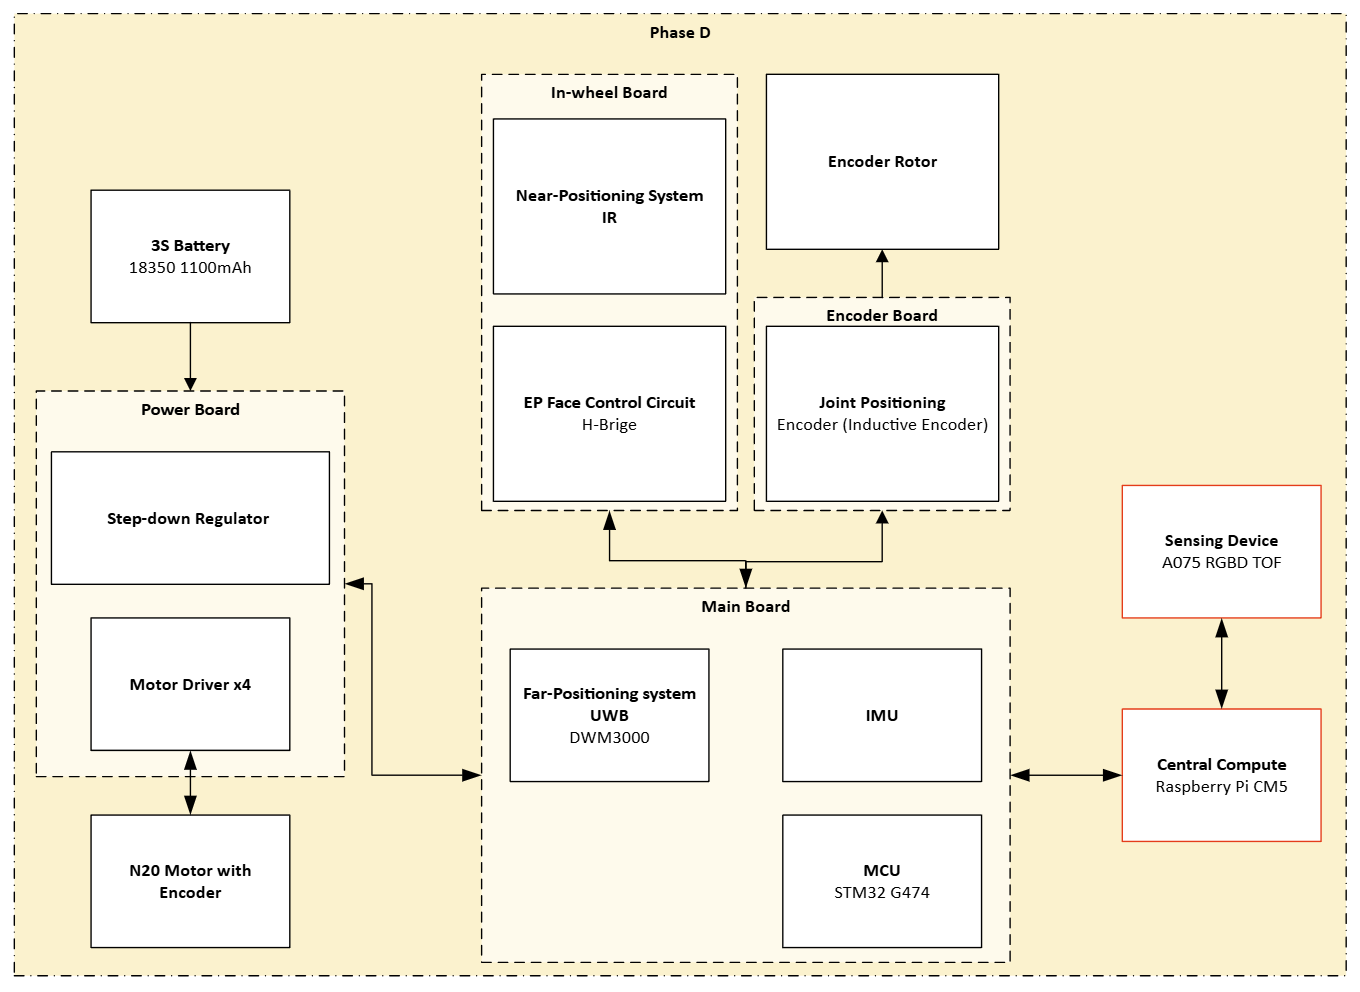
\includegraphics[width=0.78\textwidth]{../image/Phase_D_Diagram.png}
		\caption{Phase D.}
		\label{fig:phase-d}
	\end{subfigure}
	\caption{Electronics block diagrams, Phases C--D.}
	\label{fig:phase-diagrams-cd}
\end{figure}

% ----------------------------------------------------------------
\subsection{Component Selection}

\begin{table}[H]
\centering\small
\caption{Key electronics components.}
\label{tab:components}
\begin{tabular}{@{}L{0.18\textwidth} L{0.15\textwidth} L{0.35\textwidth} L{0.22\textwidth}@{}}
\toprule
\textbf{Component} & \textbf{Phase} & \textbf{Key Specs} & \textbf{Interface / Supply} \\
\midrule
4$\times$ N20 gearmotor & A-1+ & 6\,V, 50\,rpm; 7\,PPR encoder & A/B quadrature; H-bridge \\
STM32G474 & A+ & Cortex-M4F @ 170\,MHz; 12-bit ADC; FDCAN & SPI/I2C/UART/CAN; 3.3\,V \\
ICM-42688-P & A+ & $\pm$2000\,dps / $\pm$16\,g; 32\,kHz ODR & SPI or I2C; 1.8\,V \\
DW3000 (UWB) & A+ & IEEE 802.15.4z; $\sim$10\,cm ranging & SPI; 3.3\,V \\
ESP32-C3 & A-1+ & Wi-Fi 4 + BLE 5; RISC-V @ 160\,MHz & UART/SPI; 3.3\,V \\
EP-Face + IR PCB & B & Custom; EP magnet + IR alignment & Slip ring; 3.3\,V \\
RPi CM5 & D & Cortex-A76 @ 2.4\,GHz; up to 16\,GB RAM & Custom carrier; 5\,V \\
Sipeed MaixSense A075V & C+ & ToF 320$\times$240 @ 30\,fps; RGB 800$\times$600 & USB 2.0; 5\,V \\
\bottomrule
\end{tabular}
\end{table}

% ----------------------------------------------------------------
\subsection{Electronics Packaging}

All components fit within the \SI{100}{mm} cube based on rough CAD placement (Figure~\ref{fig:elec-packaging}).

\begin{figure}[!htbp]
	\centering
	\begin{subfigure}[b]{0.45\textwidth}
		\centering
		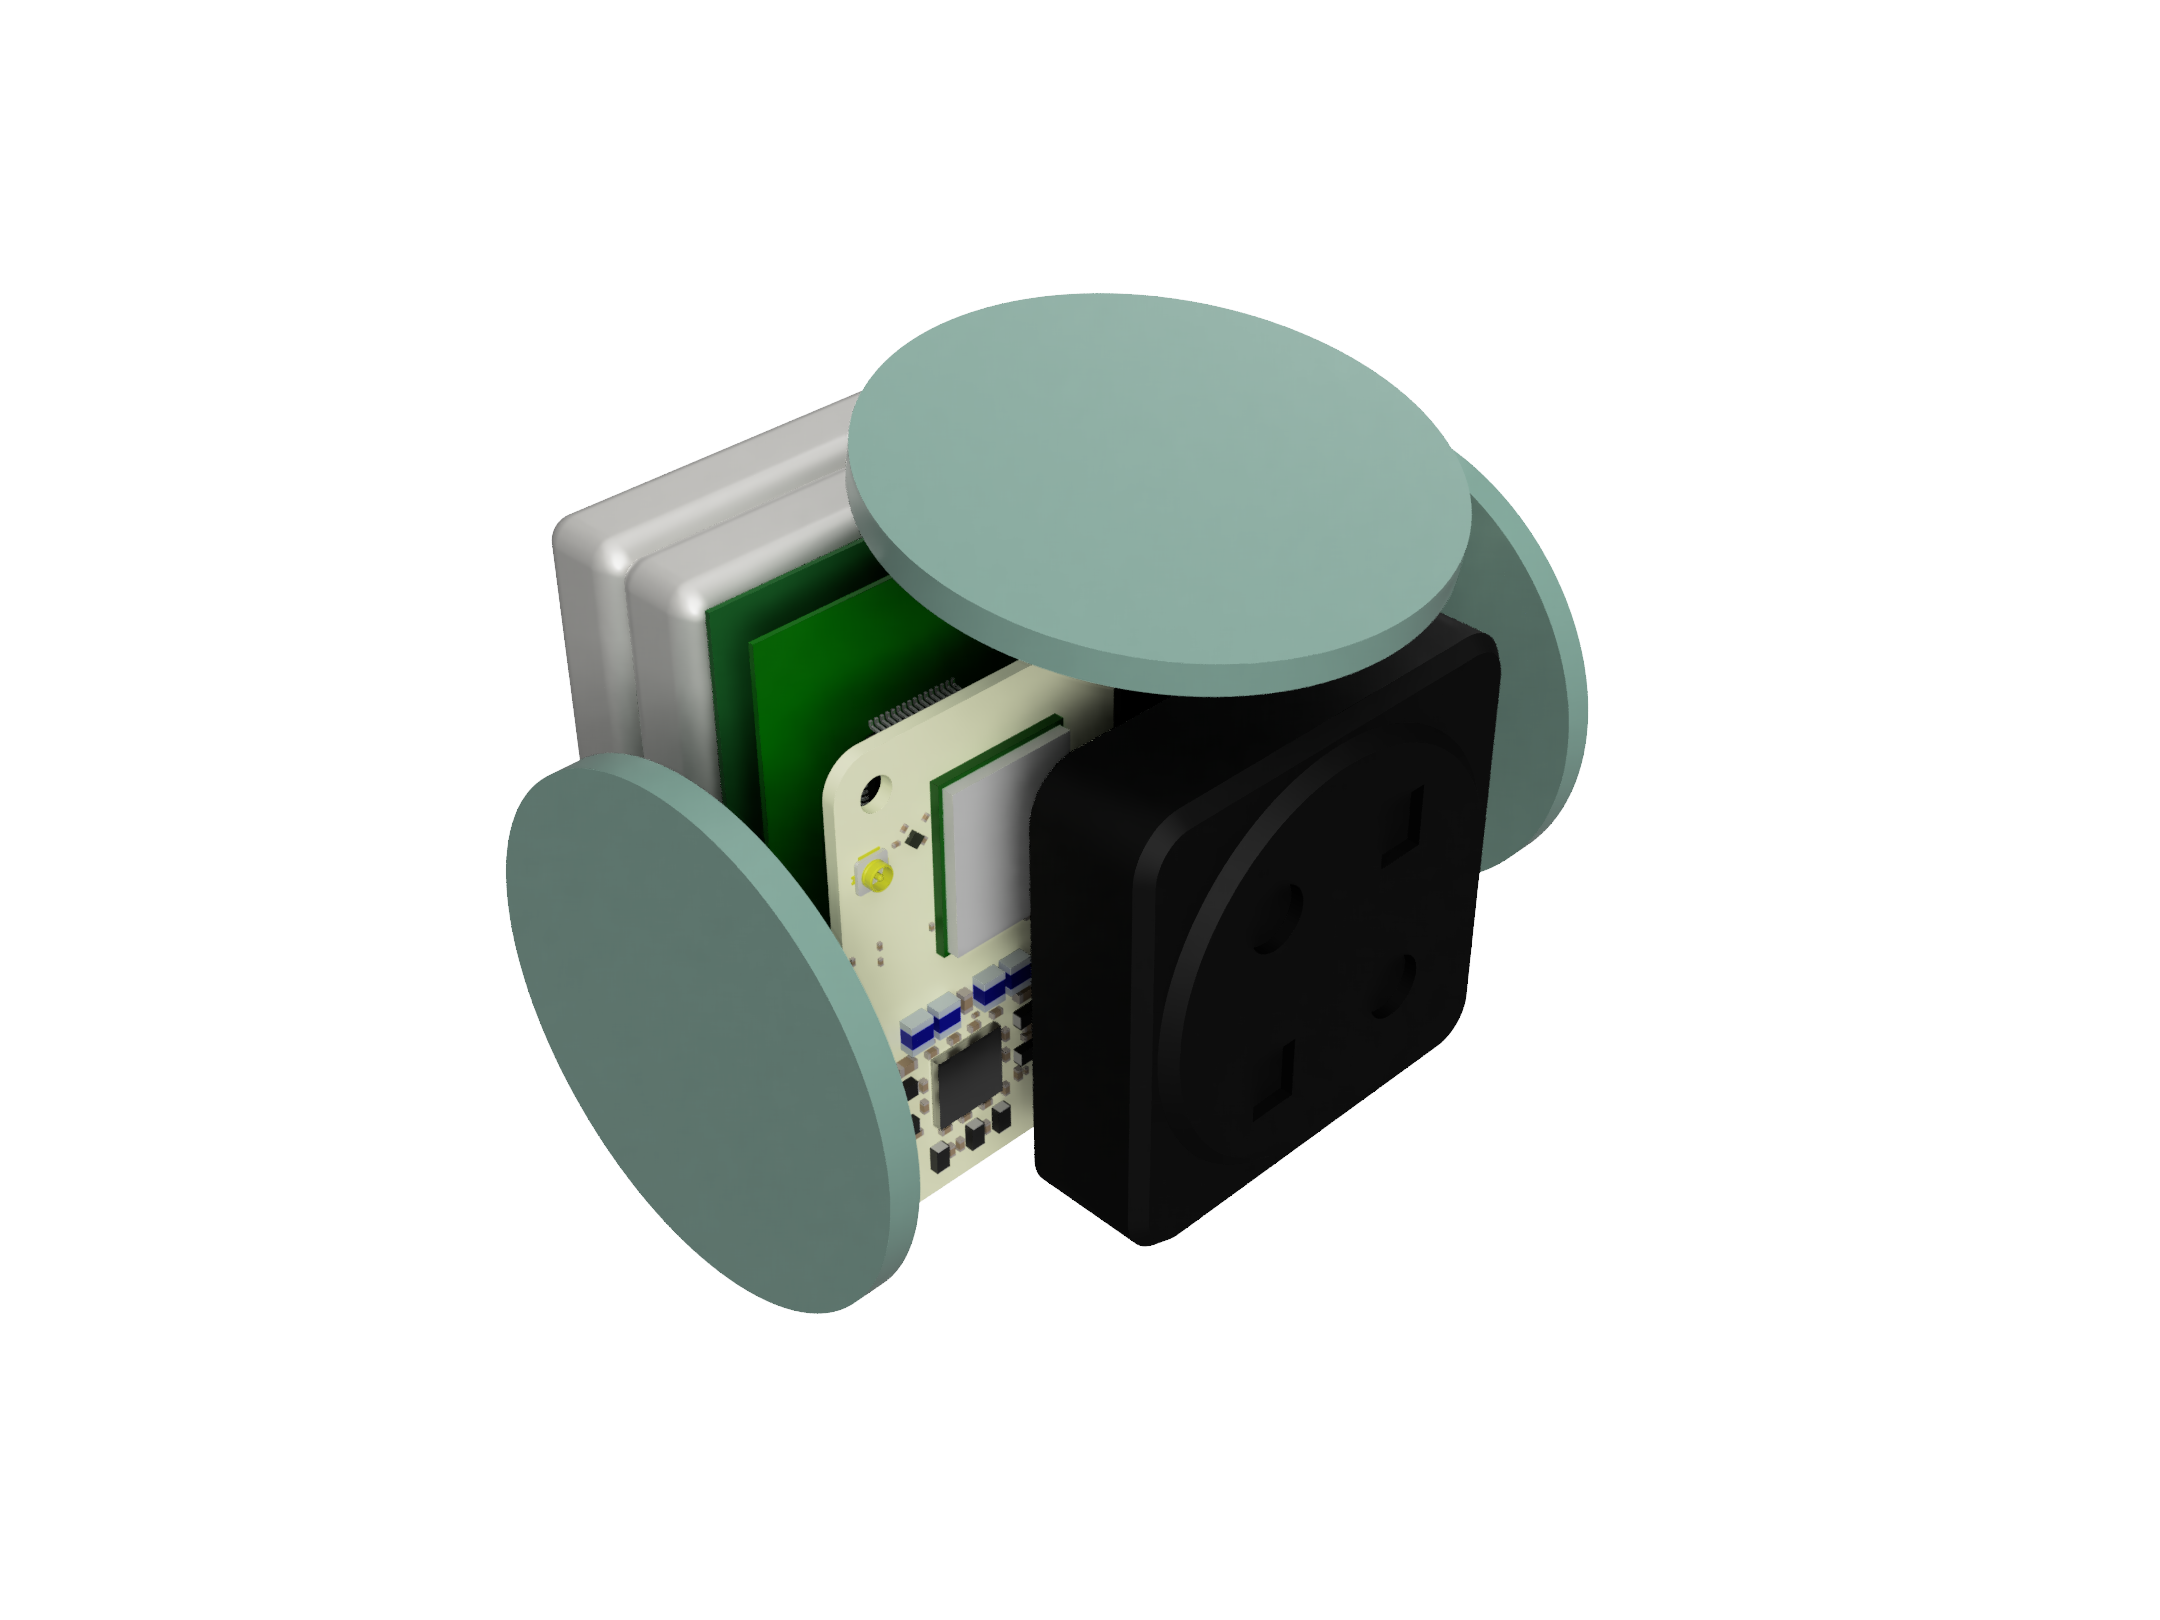
\includegraphics[width=\linewidth]{../image/Elec_Assembly.png}
		\caption{Assembled.}
		\label{fig:elec-assembly}
	\end{subfigure}
	\hfill
	\begin{subfigure}[b]{0.45\textwidth}
		\centering
		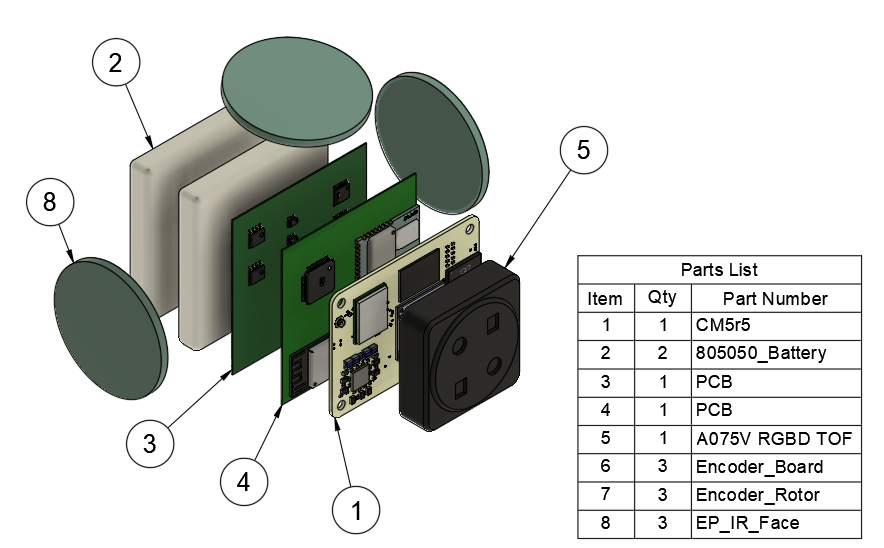
\includegraphics[width=\linewidth]{../image/Elec_Exploded_View.png}
		\caption{Exploded.}
		\label{fig:elec-exploded}
	\end{subfigure}
	\caption{Electronics packaging.}
	\label{fig:elec-packaging}
\end{figure}

% ----------------------------------------------------------------
\subsection{Wheel Encoder}

Replacing the original continuous-rotation potentiometer ($\sim$5$^\circ$ resolution, contact wear) with a non-contact encoder. Three options considered:

\begin{table}[H]
\centering\small
\caption{Wheel encoder options.}
\label{tab:encoders}
\begin{tabular}{@{}L{0.20\textwidth} L{0.24\textwidth} L{0.24\textwidth} L{0.24\textwidth}@{}}
\toprule
& \textbf{On-axis magnetic} (AS5600) & \textbf{Off-axis tape} & \textbf{Custom inductive} \\
\midrule
Output & Absolute, 12--14 bit & Incremental + index & Absolute \\
EP interference & Sensitive & Sensitive & Immune \\
Design effort & Low & Medium & High \\
\bottomrule
\end{tabular}
\end{table}

The inductive option best handles the EP connector's nearby field but has the highest schedule risk. Decision deferred to Phase C.

% ----------------------------------------------------------------
\subsection{Changes from Progress Report 1}
\label{sec:elec-changes}

The phased plan (A-1 to D) and its scope are unchanged. The electronics work
plan is delayed by one week, which shifts the electronics timeline and the
work that depends on it by the same amount.

Phase A-1 was built from an STM32F411 development board, two TB6612FNG
dual H-bridge drivers and an ESP32-C6 module, instead of the COTS 4-channel
motor driver with a built-in MCU and the ESP32-C3 described in PR1. This gives direct control of the PWM, direction
and encoder signals, so the wiring and firmware carry over to the Phase A main
board.

The only other hardware change is the battery. The 2S \SI{3000}{mAh} 505080 pack was
replaced with a 3S pack of Vapcell M11 18350 Li-ion cells (\SI{1100}{mAh},
\SI{10}{A} continuous, \SI{15}{A} burst), which can supply more current for the
EP-Face in Phase B. The smaller capacity lowers the estimated run time
(Section~\ref{sec:power-new}).

% ----------------------------------------------------------------
\subsection{Phase A-1 Hardware}
\label{sec:phase-a1-hw}

Phase A-1 is the bench version of the locomotion electronics. It tests the
wiring, power path and firmware set-up that will move onto the Phase A PCBs.

% Placeholder-safe figure: grey box until the image exists.
\providecommand{\figOrBox}[2]{%
  \IfFileExists{#2}{\includegraphics[width=#1]{#2}}%
  {\fbox{\parbox[c][0.3\textheight][c]{\dimexpr#1-2\fboxsep-2\fboxrule\relax}{\centering\small TODO: \detokenize{#2}}}}}

\subsubsection{Hardware Schematic}

Figure~\ref{fig:a1-schematic} shows the Phase A-1 wiring. An STM32F411CEU6
development board controls four N20 gearmotors through two dual-channel
TB6612FNG H-bridge drivers (two motors each, shared standby line). Each motor
has a PWM input and two direction inputs, and its quadrature encoder is read
back by the MCU. M3 and M4 drive the left and right wheels; M1 and M2, the
inner-left (iL) and inner-right (iR) motors, drive pan and tilt. An ESP32-C6 module provides the Wi-Fi link over UART,
an ST-Link handles SWD programming, and USB gives a serial console for testing.

Three buck converters run from the 3S pack through an XT30 connector. A 5\,V
buck supplies the MCU board and the ESP32-C6; the MCU board's 3.3\,V regulator
supplies the driver logic and the encoders. One 6\,V buck per TB6612FNG
supplies the motors, so the N20s run at their rated voltage at full PWM duty.
A \SI{100}{nF} capacitor across each motor suppresses brush noise, and a
\SI{10}{k\ohm} pull-down on STBY keeps both drivers disabled until the MCU
enables them.

\begin{figure}[!htbp]
  \centering
  \figOrBox{\textwidth}{../image/Phase_A1_Schematic.png}
  \caption{Phase A-1 hardware schematic.}
  \label{fig:a1-schematic}
\end{figure}

\subsubsection{Hardware Packaging}

Figure~\ref{fig:a1-cad} shows the Phase A-1 hardware placed in the module.
Three parts stack front to back inside the module shell. The three 18350 cells
sit in a vertical column at the back. In front of them is the regulator board
with the three buck converters. The controller board, carrying the STM32F411
board, both TB6612FNG drivers and the ESP32-C6, sits at the front.

\begin{figure}[!htbp]
  \centering
  \begin{subfigure}[b]{0.36\textwidth}
    \centering
    \figOrBox{\linewidth}{../image/Phase_A1_CAD.png}
    \caption{Assembled.}
  \end{subfigure}
  \hfill
  \begin{subfigure}[b]{0.6\textwidth}
    \centering
    \figOrBox{\linewidth}{../image/Phase_A1_CAD_Exploded.png}
    \caption{Exploded.}
  \end{subfigure}
  \caption{Phase A-1 hardware packaging.}
  \label{fig:a1-cad}
\end{figure}

\subsubsection{Power Calculation}

Table~\ref{tab:a1-power} gives the Phase A-1 load on the 3S pack, using the
PR1 load figures. Motor power passes through the 6\,V regulators (90\,\%) and
the TB6612FNG (95\,\%); logic power through a 5\,V buck (90\,\%) and the
board's 3.3\,V LDO (66\,\%).

\begin{table}[H]
\centering\small
\caption{Phase A-1 power budget (3S pack, \SI{9.8}{Wh} usable).}
\label{tab:a1-power}
\begin{tabular}{@{}lccc@{}}
\toprule
\textbf{Load} & \textbf{Typical} & \textbf{All motors driving} & \textbf{Peak (all stalled)} \\
\midrule
4$\times$ N20 via 6\,V reg.\ + TB6612 & 2.6\,W\textsuperscript{a} & 7.0\,W & 28.1\,W \\
STM32F411 + ESP32-C6 (3.3\,V) & 0.7\,W & 0.7\,W & 2.2\,W\textsuperscript{b} \\
\midrule
\textbf{Total from pack} & \textbf{3.3\,W} & \textbf{7.7\,W} & \textbf{30.3\,W} \\
Pack current (11.1\,V) & 0.30\,A & 0.69\,A & 2.7\,A (3.4\,A at 9\,V) \\
Run time & \textbf{3.0\,h} & \textbf{1.3\,h} & -- \\
\bottomrule
\end{tabular}

\smallskip
{\footnotesize \textsuperscript{a}PR1 duty cycle: wheels 60\,\%, pan/tilt 15\,\%, 0.25\,A each loaded.
\textsuperscript{b}Wi-Fi transmit burst, 335\,mA (PR1 ESP32-C3 figure).}
\end{table}

The 3.4\,A worst-case pack current is well inside the cell's \SI{10}{A}
continuous rating. Because the drivers see 6\,V, a stalled N20 draws about
1\,A, inside the TB6612FNG's 1.2\,A continuous rating per channel. Each 6\,V
regulator must supply up to 2\,A with both of its motors stalled.
% TODO (recommended): add measured motor and logic currents next to these.

\subsubsection{Embedded System Setup}

The STM32F411 was configured in STM32CubeMX (Figure~\ref{fig:a1-cubemx},
Table~\ref{tab:a1-periph}). The 25\,MHz crystal is multiplied by the PLL to a
96\,MHz system clock, which also gives the exact 48\,MHz needed for USB. One
timer generates the PWM for all four motors at 20\,kHz, which is above
hearing range. Each encoder has its own timer in quadrature (4$\times$) mode
with input filtering and pull-ups. A separate timer interrupt at 1\,kHz sets
the control-loop rate. The ESP32-C6 link uses DMA, with a circular receive
buffer so incoming commands are not lost while the CPU is busy.

\begin{figure}[!htbp]
  \centering
  \figOrBox{0.55\textwidth}{../image/Phase_A1_CubeMX.png}
  \caption{STM32CubeMX pin and peripheral configuration.}
  \label{fig:a1-cubemx}
\end{figure}

\begin{table}[H]
\centering\small
\caption{STM32F411 peripheral assignment.}
\label{tab:a1-periph}
\begin{tabular}{@{}lll@{}}
\toprule
\textbf{Function} & \textbf{Peripheral and pins} & \textbf{Setting} \\
\midrule
System clock & HSE 25\,MHz $\rightarrow$ PLL & 96\,MHz \\
Motor PWM, M1--M4 & TIM3 CH3/2/1/4 (PB0, PA7, PA6, PB1) & 20\,kHz \\
Motor direction & GPIO (PA4--5, PB14--15, PB12--13, PB4--5) & -- \\
Driver standby & GPIO PC15 (both TB6612) & -- \\
Encoder M1 (iL) & TIM4 (PB6, PB7), 16-bit & $\times$4 quadrature \\
Encoder M2 (iR) & TIM2 (PA15, PB3), 32-bit & $\times$4 quadrature \\
Encoder M3 (L) & TIM1 (PA8, PA9), 16-bit & $\times$4 quadrature \\
Encoder M4 (R) & TIM5 (PA0, PA1), 32-bit & $\times$4 quadrature \\
Control loop tick & TIM10 interrupt & 1\,kHz \\
ESP32-C6 link & USART2 (PA2, PA3) + DMA & 115\,200 baud \\
PC console & USB OTG FS, CDC class & -- \\
Debug & SWD (PA13, PA14) & -- \\
\bottomrule
\end{tabular}
\end{table}

% ----------------------------------------------------------------
\subsection{New Power Calculation}
\label{sec:power-new}

\begin{figure}[!htbp]
  \centering
  % TODO: re-export Power_Diagram.png with "3S 18350 1100 mAh, 9.0--12.6 V".
  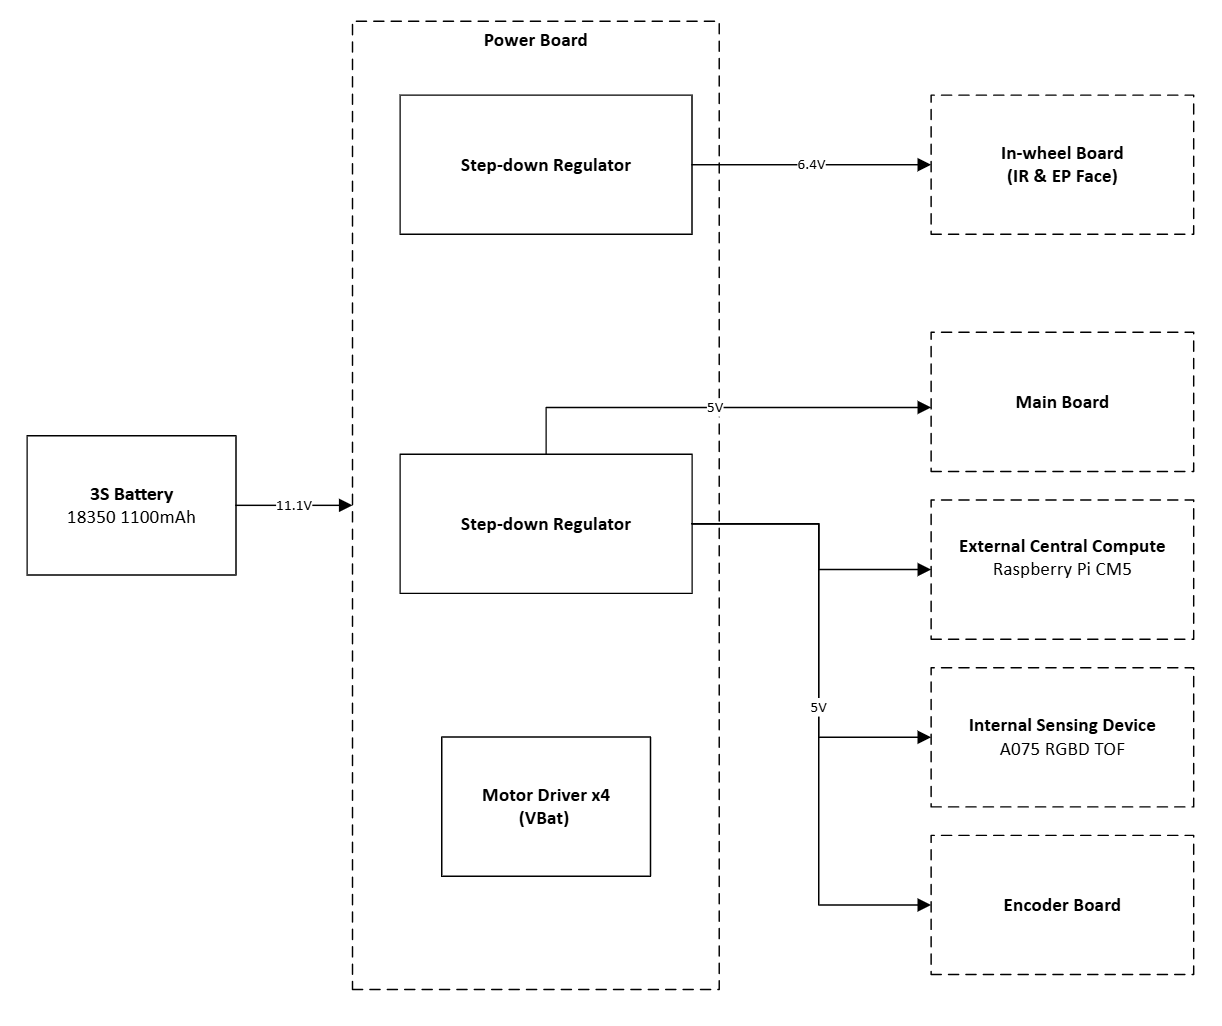
\includegraphics[width=0.6\textwidth]{../image/Power_Diagram.png}
  \caption{Power distribution block diagram.}
  \label{fig:power-diagram}
\end{figure}

The PR1 load budget is unchanged; only the pack changes. The Phase A power
board keeps the PR1 architecture: the H-bridges run directly from the pack,
not from the 6\,V regulator used on the Phase A-1 bench set-up. This removes
the regulator loss and a 4\,A regulator from the board. Power from the 3S
pack splits three ways:
\begin{itemize}
  \item \textbf{Motors:} 4$\times$ N20 via H-bridges, PWM capped at
        $\sim$48\,\% ($6/12.6$\,V at full charge) for the 6\,V rating.
  \item \textbf{EP-Face:} Dedicated buck regulator isolates pulse transients
        from the logic rail.
  \item \textbf{Logic/compute:} Buck to 5\,V (CM5, camera); LDO to 3.3\,V
        (MCU, sensors, radios).
\end{itemize}

\begin{table}[H]
\centering\small
\caption{Battery comparison, PR1 vs.\ PR2 (80\,\% of energy usable).}
\label{tab:battery-change}
\begin{tabular}{@{}lcc@{}}
\toprule
 & \textbf{PR1: 2S 505080} & \textbf{PR2: 3S Vapcell M11} \\
\midrule
Voltage (nominal / full / cutoff) & 7.4 / 8.4 / 6.6\,V & 11.1 / 12.6 / 9.0\,V \\
Capacity / energy (usable) & 3000\,mAh / 22.2\,Wh (17.8) & 1100\,mAh / 12.2\,Wh (9.8) \\
Run time, Phase A--B ($\sim$3.1\,W) & 5.8\,h & \textbf{3.2\,h} \\
Run time, Phase D ($\sim$11.5\,W) & 1.5\,h & \textbf{0.85\,h} \\
Peak current ($\sim$47\,W) & 7.1\,A (2.4\,C) & 5.2\,A (4.7\,C, cell rated 10\,A) \\
Motor PWM cap for 6\,V & $\sim$70\,\% & $\sim$48\,\% \\
H-bridge on-time stall current & 1.4\,A/ch & 2.1\,A/ch \\
\bottomrule
\end{tabular}
\end{table}

\begin{table}[H]
\centering\small
\caption{Maximum load per rail.}
\label{tab:rail-max}
\begin{tabular}{@{}lcc@{}}
\toprule
\textbf{Rail} & \textbf{Max Current} & \textbf{Max Power} \\
\midrule
Motor drive (PWM to 6\,V) & 4.0\,A (6\,V eq.); 2.1\,A/ch at 12.6\,V & 24\,W \\
5\,V logic/compute & 4.0\,A & 20\,W \\
3.3\,V (from 5\,V LDO) & 0.45\,A & 1.5\,W \\
EP-Face + IR & TBD & TBD \\
\midrule
\textbf{Pack total (peak)} & $\sim$4.2\,A @ 11.1\,V; $\sim$5.2\,A @ 9.0\,V & $\sim$47\,W \\
\bottomrule
\end{tabular}
\end{table}

Run time roughly halves, which is acceptable for lab testing in Phases A--C.
The higher pack voltage sets new ratings for the power board: H-bridges for at
least 2.1\,A per channel and a supply above 12.6\,V with margin, and buck
regulators with a 9--12.6\,V input range.

% ----------------------------------------------------------------
\subsection{Next Steps}
\label{sec:elec-next}

The tested Phase A-1 wiring and CubeMX configuration are carried over to
design the Phase A main board and power board PCBs, with:
\begin{itemize}
  \item H-bridges and buck regulators rated for the 3S pack
        (Section~\ref{sec:power-new}).
  \item The Phase A-1 pin map (Table~\ref{tab:a1-periph}) as the starting
        point for the main-board pin-out.
\end{itemize}

\subsection{programming and debugging}


\clearpage
% ================================================================
\section{Shaft Tolerance Analysis ($\varnothing$\SI{55}{mm} Bearing)}
\label{sec:shaft-tolerance}
% ================================================================

The plain bearing (OD = \SI{55}{mm}) acts as the shaft. All PETG-printed components have bores around it.

\begin{figure}[!htbp]
	\centering
	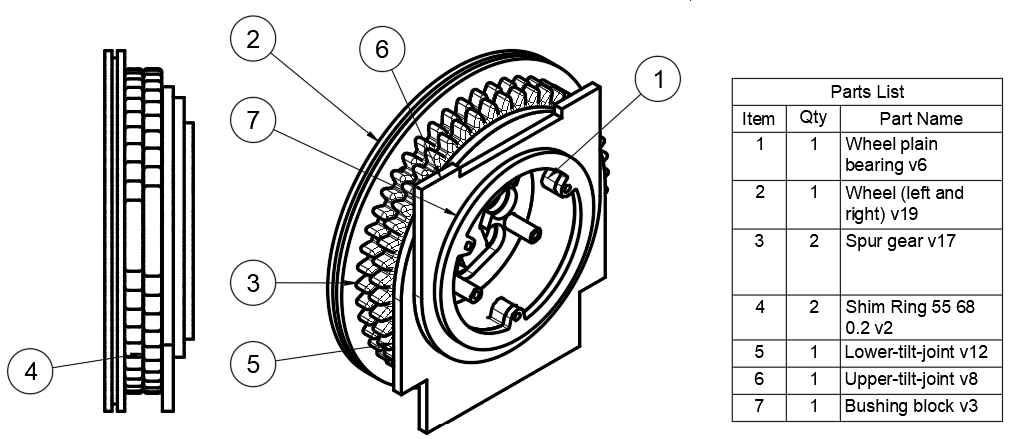
\includegraphics[width=0.6\textwidth]{../image/shaft_component.png}
	\caption{Shaft and bearing component arrangement.}
	\label{fig:shaft-component}
\end{figure}

\begin{table}[H]
\centering
\caption{Joint classification and ISO fits for $\varnothing$\SI{55}{mm} bearing.}
\label{tab:shaft-joints}
\begin{tabular}{@{}cllll@{}}
\toprule
\textbf{Joint} & \textbf{Component} & \textbf{Motion} & \textbf{Fit} & \textbf{ISO Class} \\
\midrule
J1 & Wheel + 1\textsuperscript{st} Spur Gear & Dynamic & Clearance & F7/h6 \\
J2 & 2\textsuperscript{nd} Spur Gear (Pan/Tilt) & Dynamic & Clearance & F7/h6 \\
J3 & Upper Tilt Joint & Dynamic & Clearance & F7/h6 \\
J4 & Lower Tilt Joint & \textbf{Static} & \textbf{Interference} & P7/h6 \\
\bottomrule
\end{tabular}
\end{table}

\textbf{ISO\,286 limits} (bearing h6: $55.000$--$54.981$\,mm): Dynamic F7 bore $55.030$--$55.060$\,mm (clearance $+0.030$ to $+0.079$\,mm); Static P7 bore $54.938$--$54.968$\,mm (interference $+0.013$ to $+0.062$\,mm).

\textbf{FDM print compensation:} Printed holes come out undersized, so the ISO limits cannot be used directly as CAD dimensions. The analysis above was used as the starting point for a printed-fit test. PETG was chosen over nylon because it prints easily and the mechanical design is not a focus of this project.

\textbf{Test result:} A CAD bore of $\varnothing 55.00 + 0.15 = \varnothing$\SI{55.15}{mm} was tested on the printed PETG parts and works. This single offset is adopted for \textbf{all} components on the shaft (wheel, spur gears, upper and lower tilt joints), replacing the separate dynamic and static bore sizes originally proposed (Table~\ref{tab:shaft-final}).

\begin{table}[H]
\centering
\caption{Final CAD bore size (tested).}
\label{tab:shaft-final}
\begin{tabular}{@{}llc@{}}
\toprule
\textbf{Part} & \textbf{Joint} & \textbf{CAD Bore (mm)} \\
\midrule
Wheel / Spur Gears / Upper Tilt & J1--J3 & $\varnothing 55.15$ \\
Lower Tilt Joint & J4 & $\varnothing 55.15$ \\
\bottomrule
\multicolumn{3}{@{}l}{\footnotesize Bearing OD = $\varnothing 55.00$\,mm; offset $+0.15$\,mm on all bores.}
\end{tabular}
\end{table}

\clearpage
% ================================================================
\section{Teleoperation Architecture}
\label{sec:teleop-architecture}
% ================================================================

Since Progress Report 2 the teleoperation stack has been brought up on the real module, and
the module now drives on its wheels from ROS~2 velocity commands. The PC--module link was
changed from the planned custom \texttt{ros2\_control} plugin with a UDP bridge to
micro-ROS \cite{microros}, the kinematics moved onto the module's ESP32-C6, and the STM32F411
firmware was completed for all four motors. Figure~\ref{fig:teleop-architecture} shows the
new architecture, which replaces the PR2 architecture figure. The subsections below describe
both firmwares and the test results.

\subsection{Changes from Progress Report 2}

Table~\ref{pr3:tab:changes} lists the changes made to the embedded design since PR2.
The hardware (STM32F411 board, two TB6612FNG drivers, ESP32-C6, four N20 gearmotors)
is unchanged. The changes are in the software architecture and in corrections found
during bring-up.

\begin{table}[H]
\centering
\caption{Embedded-system changes from PR2 to PR3.}
\label{pr3:tab:changes}
\small
\begin{tabularx}{\linewidth}{>{\raggedright\arraybackslash}p{3.0cm} >{\raggedright\arraybackslash}X >{\raggedright\arraybackslash}X}
\toprule
Item & PR2 & PR3 (current) \\
\midrule
PC--module link &
  Custom \texttt{ros2\_control} plugin (\texttt{mrr\_hardware}) packs wheel targets into UDP packets;
  the ESP32 is a transparent Wi-Fi$\leftrightarrow$UART bridge. &
  \textbf{micro-ROS}: the ESP32-C6 is a ROS~2 node that talks to a micro-ROS agent on the PC
  (Wi-Fi, UDP). \\
Where kinematics run &
  PC (\texttt{diff\_drive\_controller}). &
  ESP32-C6 on each module (wheel IK/FK and pan/tilt mixing). \\
Low-level control &
  Wheel speed PID only (M1, M2). &
  All four motors; cascaded position/velocity control; four modes. \\
Motor numbering &
  M1, M2 = wheels; M3, M4 = inner (pan/tilt). &
  M3\_L, M4\_R = wheels; M1\_iL, M2\_iR = inner spur gears (Table~\ref{pr3:tab:pins}). \\
Driver standby pin &
  PB10. &
  \textbf{PC15} (checked on the wired board; Table~\ref{tab:a1-periph} corrected). \\
Wheel separation &
  \SI{96.65}{mm} (measured from the CAD meshes). &
  \SI{99.9}{mm} (re-measured on the assembled module). \\
\bottomrule
\end{tabularx}
\end{table}

% ----------------------------------------------------------------------
\subsection{System Architecture}
% ----------------------------------------------------------------------

The architecture (Figure~\ref{fig:teleop-architecture}) has three processing levels,
each with one job:

\begin{enumerate}
  \item \textbf{PC (ROS~2 Humble)} decides \emph{what} the module should do. Commander
        nodes publish body-level commands: a teleoperation node in the current tests, and
        later \texttt{msrr\_control} from Section~\ref{sec:sim-model}. The micro-ROS agent forwards them to the module.
  \item \textbf{ESP32-C6 (micro-ROS node)} converts body commands into joint targets.
        It runs the inverse kinematics, enforces the command timeout and joint limits,
        and publishes feedback computed with forward kinematics.
  \item \textbf{STM32F411 (bare-metal, HAL)} makes each motor follow its target. It
        reads the four quadrature encoders, runs the PID loops at \SI{1}{kHz} and
        drives the TB6612FNG H-bridges with \SI{20}{kHz} PWM.
\end{enumerate}

\begin{figure}[p]
\centering
\resizebox{\linewidth}{!}{%
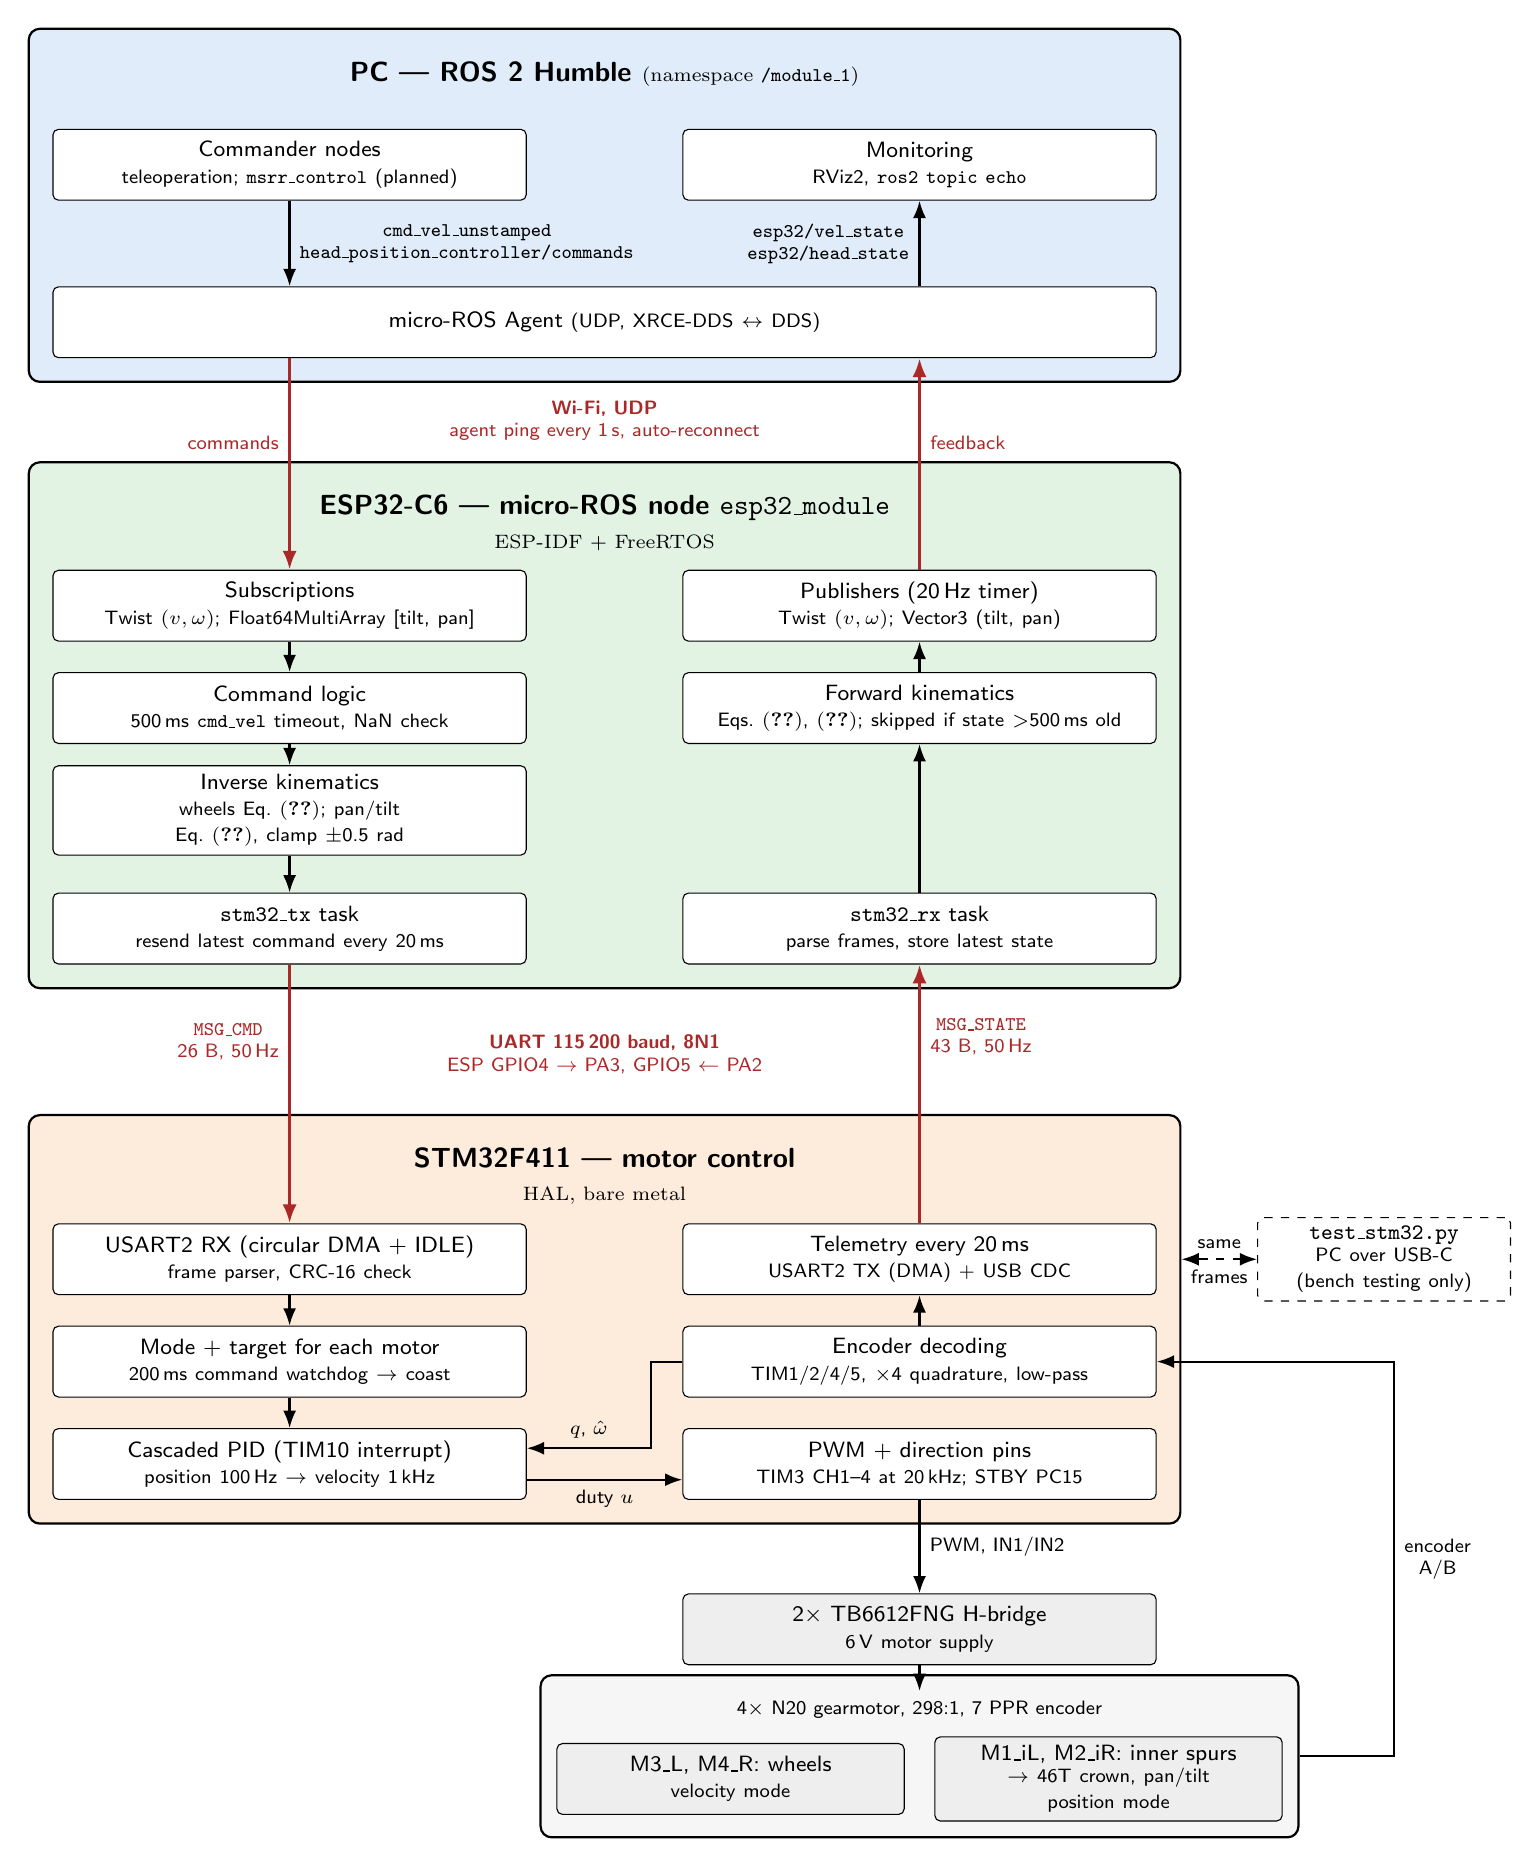
\begin{tikzpicture}[
  font=\sffamily\footnotesize,
  blk/.style={draw, rounded corners=2pt, fill=white, align=center, text width=58mm, minimum height=9mm, inner sep=3pt},
  grp/.style={draw, rounded corners=4pt, inner sep=3mm, thick},
  ttl/.style={font=\sffamily\bfseries, align=center},
  arr/.style={-{Latex[length=2.2mm]}, thick},
  red/.style={-{Latex[length=2.4mm]}, very thick, linkred},
  note/.style={font=\sffamily\scriptsize, align=center},
]
% ---------------- PC ----------------
\node[ttl] (pct) at (4,1.15) {PC --- ROS 2 Humble \normalfont\scriptsize(namespace \texttt{/module\_1})};
\node[blk] (cmdr) at (0,0) {Commander nodes\\ \scriptsize teleoperation; \texttt{msrr\_control} (planned)};
\node[blk] (mon)  at (8,0) {Monitoring\\ \scriptsize RViz2, \texttt{ros2 topic echo}};
\node[blk, text width=138mm] (agent) at (4,-2.0) {micro-ROS Agent \scriptsize(UDP, XRCE-DDS $\leftrightarrow$ DDS)};
\draw[arr] (cmdr.south) -- node[note, right] {\texttt{cmd\_vel\_unstamped}\\\texttt{head\_position\_controller/commands}} (cmdr.south |- agent.north);
\draw[arr] (mon.south |- agent.north) -- node[note, left] {\texttt{esp32/vel\_state}\\\texttt{esp32/head\_state}} (mon.south);
\begin{scope}[on background layer]
\node[grp, fill=pcblue, fit=(pct)(cmdr)(mon)(agent)] (pc) {};
\end{scope}

% ---------------- ESP32 ----------------
\node[ttl] (espt) at (4,-4.55) {ESP32-C6 --- micro-ROS node \texttt{esp32\_module}\\ \normalfont\scriptsize ESP-IDF + FreeRTOS};
\node[blk] (subs)  at (0,-5.6)  {Subscriptions\\ \scriptsize Twist $(v,\omega)$; Float64MultiArray [tilt, pan]};
\node[blk] (logic) at (0,-6.9)  {Command logic\\ \scriptsize 500\,ms \texttt{cmd\_vel} timeout, NaN check};
\node[blk] (ik)    at (0,-8.2)  {Inverse kinematics\\ \scriptsize wheels Eq.~\eqref{pr3:eq:ik}; pan/tilt Eq.~\eqref{pr3:eq:ptik}, clamp $\pm$0.5 rad};
\node[blk] (tx)    at (0,-9.7)  {\texttt{stm32\_tx} task\\ \scriptsize resend latest command every 20\,ms};
\node[blk] (pubs)  at (8,-5.6)  {Publishers (20\,Hz timer)\\ \scriptsize Twist $(v,\omega)$; Vector3 (tilt, pan)};
\node[blk] (fk)    at (8,-6.9)  {Forward kinematics\\ \scriptsize Eqs.~\eqref{pr3:eq:fk}, \eqref{pr3:eq:ptfk}; skipped if state $>$500\,ms old};
\node[blk] (rx)    at (8,-9.7)  {\texttt{stm32\_rx} task\\ \scriptsize parse frames, store latest state};
\draw[arr] (subs) -- (logic);
\draw[arr] (logic) -- (ik);
\draw[arr] (ik) -- (tx);
\draw[arr] (rx) -- (fk);
\draw[arr] (fk) -- (pubs);
\begin{scope}[on background layer]
\node[grp, fill=espgreen, fit=(espt)(subs)(tx)(pubs)(rx)] (esp) {};
\end{scope}

% PC <-> ESP link
\draw[red] (cmdr.south |- agent.south) -- node[note, left, text=linkred, pos=0.4] {commands} (subs.north);
\draw[red] (pubs.north) -- node[note, right, text=linkred, pos=0.6] {feedback} (mon.south |- agent.south);
\node[note, text=linkred] at (4,-3.25) {\textbf{Wi-Fi, UDP}\\ agent ping every 1\,s, auto-reconnect};

% ---------------- STM32 ----------------
\node[ttl] (stmt) at (4,-12.85) {STM32F411 --- motor control\\ \normalfont\scriptsize HAL, bare metal};
\node[blk] (parse) at (0,-13.90) {USART2 RX (circular DMA + IDLE)\\ \scriptsize frame parser, CRC-16 check};
\node[blk] (wd)    at (0,-15.20) {Mode + target for each motor\\ \scriptsize 200\,ms command watchdog $\rightarrow$ coast};
\node[blk] (pid)   at (0,-16.50) {Cascaded PID (TIM10 interrupt)\\ \scriptsize position 100\,Hz $\rightarrow$ velocity 1\,kHz};
\node[blk] (tele)  at (8,-13.90) {Telemetry every 20\,ms\\ \scriptsize USART2 TX (DMA) + USB CDC};
\node[blk] (enc)   at (8,-15.20) {Encoder decoding\\ \scriptsize TIM1/2/4/5, $\times$4 quadrature, low-pass};
\node[blk] (pwm)   at (8,-16.50) {PWM + direction pins\\ \scriptsize TIM3 CH1--4 at 20\,kHz; STBY PC15};
\draw[arr] (parse) -- (wd);
\draw[arr] (wd) -- (pid);
\draw[arr] ([yshift=-2mm]pid.east) -- node[note, below] {duty $u$} ([yshift=-2mm]pwm.west);
\draw[arr] (enc.west) -- ++(-0.4,0) |- node[note, pos=0.75, above] {$q$, $\hat\omega$} ([yshift=2mm]pid.east);
\draw[arr] (enc) -- (tele);
\begin{scope}[on background layer]
\node[grp, fill=stmorange, fit=(stmt)(parse)(pid)(tele)(pwm)] (stm) {};
\end{scope}

% ESP <-> STM link
\draw[red] (tx.south) -- node[note, left, text=linkred, pos=0.3] {\texttt{MSG\_CMD}\\26 B, 50\,Hz} (parse.north);
\draw[red] (tele.north) -- node[note, right, text=linkred, pos=0.72] {\texttt{MSG\_STATE}\\43 B, 50\,Hz} (rx.south);
\node[note, text=linkred] at (4,-11.3) {\textbf{UART 115\,200 baud, 8N1}\\ ESP GPIO4 $\rightarrow$ PA3, GPIO5 $\leftarrow$ PA2};

% USB bench tool
\node[blk, dashed, text width=30mm] (usb) at (13.9,-13.90) {\texttt{test\_stm32.py}\\ \scriptsize PC over USB-C\\(bench testing only)};
\draw[dashed, thick, {Latex[length=2.2mm]}-{Latex[length=2.2mm]}] (usb.west) -- node[note, above] {same} node[note, below] {frames} (stm.east |- usb.west);

% ---------------- Hardware ----------------
\node[blk, fill=hwgray] (tb) at (8,-18.60) {2$\times$ TB6612FNG H-bridge\\ \scriptsize 6\,V motor supply};
\node[blk, fill=hwgray, text width=42mm] (wheels) at (5.6,-20.50) {M3\_L, M4\_R: wheels\\ \scriptsize velocity mode};
\node[blk, fill=hwgray, text width=42mm] (inner)  at (10.4,-20.50) {M1\_iL, M2\_iR: inner spurs\\ \scriptsize $\rightarrow$ 46T crown, pan/tilt\\ \scriptsize position mode};
\node[font=\sffamily\scriptsize, anchor=south] (motl) at (8,-19.85) {4$\times$ N20 gearmotor, 298:1, 7 PPR encoder};
\begin{scope}[on background layer]
\node[grp, fill=hwgray!50, fit=(wheels)(inner)(motl), inner sep=2mm] (mot) {};
\end{scope}
\draw[arr] (pwm) -- node[note, right] {PWM, IN1/IN2} (tb);
\draw[arr] (tb) -- (motl.north);
\draw[arr] (mot.east) -- ++(1.2,0) |- node[note, pos=0.25, right] {encoder\\A/B} (enc.east);
\end{tikzpicture}}
\caption{Teleoperation and embedded system architecture (replaces the architecture figure of Progress Report~2). The PC sends
body-level commands through micro-ROS; each module's ESP32-C6 computes the joint targets and
the STM32F411 closes the motor loops. Red arrows are the two communication links. The dashed
USB path is used only for bench testing without the ESP32.}
\label{fig:teleop-architecture}
\end{figure}

\paragraph{Why micro-ROS.} PR2 planned a custom \texttt{ros2\_control} hardware plugin on the
PC that packed wheel targets into UDP packets, with the ESP32 only forwarding bytes to the
STM32. With micro-ROS the ESP32-C6 becomes a normal ROS~2 node instead:
\begin{itemize}
  \item No custom PC plugin or custom UDP packet format has to be written and maintained.
        The module's topics appear in the ROS graph and can be inspected with standard tools
        (\texttt{ros2 topic list}, \texttt{ros2 topic echo}), which makes debugging easier.
  \item The command topics have the \emph{same names and message types} as the controllers in
        the Gazebo simulation (Table~\ref{tab:sim-joints}). A commander node can therefore drive the simulated or the real
        module without changes (tested so far with teleoperation only).
  \item Kinematics run on each module, and the PC sends only body-level commands. This fits
        the distributed SMORES-EP design and scales to $N$ modules, one namespace each
        (\texttt{/module\_1}, \texttt{/module\_2}, \dots). It is also a step towards the onboard
        computation of Phase~D.
  \item The micro-ROS session is checked with a ping every second and is re-created
        automatically when the connection returns (Section~\ref{pr3:sec:agent}).
\end{itemize}
Two trade-offs were accepted. The module namespace and the agent IP address are build-time
settings, so each module currently needs its own build. On hardware the module publishes its
measured velocity on \texttt{esp32/vel\_state} instead of \texttt{ros2\_control} producing
\texttt{/odom} and \texttt{/joint\_states}.

% ----------------------------------------------------------------------
\subsection{ROS 2 Interface}
% ----------------------------------------------------------------------

Table~\ref{pr3:tab:topics} lists the module's ROS~2 interface. All names are relative to the
module namespace (\texttt{/module\_1} for the first module).

\begin{table}[H]
\centering
\caption{ROS~2 topics of the micro-ROS node \texttt{esp32\_module}.}
\label{pr3:tab:topics}
\small
\begin{tabularx}{\linewidth}{l c >{\raggedright\arraybackslash}X}
\toprule
Topic and message type & Dir. & Content \\
\midrule
\texttt{diff\_drive\_controller/cmd\_vel\_unstamped} & sub & \texttt{linear.x} $=v$ [m/s], \texttt{angular.z} $=\omega$ [rad/s] \\
\quad\footnotesize\texttt{geometry\_msgs/Twist} & & \\[2pt]
\texttt{head\_position\_controller/commands} & sub & \texttt{data} $=[\theta_\text{tilt},\theta_\text{pan}]$ [rad] \\
\quad\footnotesize\texttt{std\_msgs/Float64MultiArray} & & \\[2pt]
\texttt{esp32/vel\_state} & pub & measured $v$, $\omega$ from the wheel encoders, 20\,Hz \\
\quad\footnotesize\texttt{geometry\_msgs/Twist} & & \\[2pt]
\texttt{esp32/head\_state} & pub & \texttt{x} $=\theta_\text{tilt}$, \texttt{y} $=\theta_\text{pan}$ [rad], 20\,Hz \\
\quad\footnotesize\texttt{geometry\_msgs/Vector3} & & \\
\bottomrule
\end{tabularx}
\end{table}

% ----------------------------------------------------------------------
\subsection{ESP32-C6 Firmware}
\label{pr3:sec:esp}
% ----------------------------------------------------------------------

The firmware (ESP-IDF project \texttt{smores\_esp32c6}) uses the micro-ROS component for
ESP-IDF on the Humble branch (\texttt{micro\_ros\_espidf\_component} \texttt{\^{}22}) with the
default XRCE-DDS middleware over Wi-Fi. The Wi-Fi network and the agent's IP address and
port are set in \texttt{menuconfig}. It is split into the files in Table~\ref{pr3:tab:espfiles}
and runs the FreeRTOS tasks in Table~\ref{pr3:tab:esptasks}.

\begin{table}[H]
\centering
\caption{ESP32-C6 source files.}
\label{pr3:tab:espfiles}
\small
\begin{tabularx}{\linewidth}{l >{\raggedright\arraybackslash}X}
\toprule
File & Purpose \\
\midrule
\texttt{robot\_config.h} & All per-module settings: namespace, topic names, UART pins, timing, wheel radius and separation, pan/tilt gains and limits \\
\texttt{main.c} & micro-ROS entities, subscription callbacks, 20\,Hz feedback timer, agent connection state machine \\
\texttt{robot\_logic.c} & Stores the latest commands and builds the 4-motor STM32 command (mode + target), including the \texttt{cmd\_vel} timeout \\
\texttt{kinematics.c} & Differential-drive and pan/tilt inverse and forward kinematics \\
\texttt{stm32\_link.c} & UART driver and the RX/TX tasks; shares the latest command and state under a spinlock \\
\texttt{protocol.c} & Frame builder and byte-by-byte parser with CRC-16 (same file as on the STM32) \\
\bottomrule
\end{tabularx}
\end{table}

\begin{table}[H]
\centering
\caption{FreeRTOS tasks on the ESP32-C6 (micro-ROS task values are the project defaults in \texttt{Kconfig.projbuild}).}
\label{pr3:tab:esptasks}
\small
\begin{tabularx}{\linewidth}{l c c >{\raggedright\arraybackslash}X}
\toprule
Task & Priority & Stack & Work \\
\midrule
\texttt{uros\_task}  & 5 & \SI{16000}{B} & micro-ROS executor (2 subscriptions + 1 timer), agent ping and reconnection \\
\texttt{stm32\_tx}   & 6 & \SI{3072}{B}  & Sends the latest \texttt{MSG\_CMD} every \SI{20}{ms} (\texttt{vTaskDelayUntil}) \\
\texttt{stm32\_rx}   & 6 & \SI{3072}{B}  & Reads the UART, parses frames, stores the latest \texttt{MSG\_STATE}; 1\,Hz debug log \\
\bottomrule
\end{tabularx}
\end{table}

The callbacks only store the new command and rebuild the STM32 command; the
\texttt{stm32\_tx} task sends it. Sending at a fixed \SI{50}{Hz}, independent of how often
ROS publishes, keeps the STM32 watchdog (\SI{200}{ms}) fed while the PC is connected.

\subsubsection{Wheel Kinematics}

With wheel radius $r=\SI{50}{mm}$ and wheel separation $L=\SI{99.9}{mm}$, the inverse
kinematics give the wheel angular velocities from the body command $(v,\omega)$:
\begin{equation}
  \omega_L = \frac{v-\omega L/2}{r}, \qquad \omega_R = \frac{v+\omega L/2}{r}.
  \label{pr3:eq:ik}
\end{equation}
The installed wheels turn opposite to the ROS convention, so both targets are multiplied
by a sign $s_\text{drive}=-1$ before they are sent; the encoder signs are not changed.
The measured wheel velocities are converted back with the forward kinematics:
\begin{equation}
  v = \frac{r}{2}\,(\omega_R+\omega_L), \qquad \omega = \frac{r}{L}\,(\omega_R-\omega_L).
  \label{pr3:eq:fk}
\end{equation}
As a check, the top speed in Section~\ref{sec:sim-model} ($v=\SI{0.049}{m/s}$) gives
$\omega_L=\omega_R=\SI{0.98}{rad/s}$ at the wheel. This equals the free speed of the
48T spur gear (\SI{50}{rpm} N20 output $\times\,9/48 = \SI{9.4}{rpm}$).

\subsubsection{Pan/Tilt Kinematics}

The pan/tilt mixing equation in Section~\ref{sec:sim-model} left the mixing to the firmware; it is now implemented on the ESP32.
Let $q_\text{iL}$ and $q_\text{iR}$ be the angles of the two inner 48T spur gears. Turning
both the same way tilts the face; turning them in opposite directions spins the 46T crown
gear (pan):
\begin{equation}
  q_\text{iL} = \frac{\theta_\text{tilt}}{K_t} + \frac{\theta_\text{pan}}{K_p}, \qquad
  q_\text{iR} = \frac{\theta_\text{tilt}}{K_t} - \frac{\theta_\text{pan}}{K_p},
  \label{pr3:eq:ptik}
\end{equation}
\begin{equation}
  \theta_\text{tilt} = K_t\,\frac{q_\text{iL}+q_\text{iR}}{2}, \qquad
  \theta_\text{pan}  = K_p\,\frac{q_\text{iL}-q_\text{iR}}{2},
  \label{pr3:eq:ptfk}
\end{equation}
with $K_t=1$ and $K_p=48/46$, the same relation as in the simulation's
\texttt{ros2\_control} xacro. In the notation of that equation this is $N_t=1$ and
$N_p=46/48$ at the spur-gear level; the remaining motor-to-spur reduction
($298\times48/9$) is handled by the encoder scaling on the STM32 (Eq.~\eqref{pr3:eq:cpr}).
Before Eq.~\eqref{pr3:eq:ptik} is applied, $\theta_\text{pan}$ and $\theta_\text{tilt}$ are
clamped to $\pm\SI{0.5}{rad}$, a conservative range for first tests.

\subsubsection{Agent Connection Handling}
\label{pr3:sec:agent}

The micro-ROS task follows the reconnection pattern of Figure~\ref{pr3:fig:agent}. ROS entities
(node, subscriptions, publishers, timer, executor) exist only while the agent answers.
When the agent is lost they are destroyed without waiting for the agent, and the task
goes back to waiting. While it waits, the task keeps applying the \texttt{cmd\_vel} timeout,
so the wheels are commanded to \SI{0}{rad/s} instead of repeating the last command.

\begin{figure}[H]
\centering
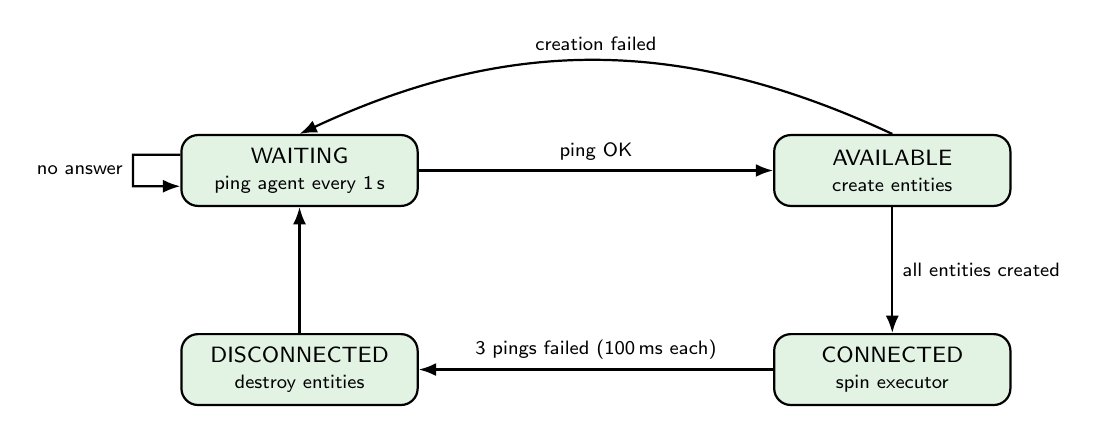
\begin{tikzpicture}[
  font=\sffamily\footnotesize, node distance=16mm and 45mm,
  st/.style={draw, rounded corners=6pt, thick, minimum width=30mm, minimum height=9mm, align=center, fill=espgreen},
  arr/.style={-{Latex[length=2.2mm]}, thick},
  tl/.style={font=\sffamily\scriptsize, align=center}
]
\node[st] (w) {WAITING\\ \scriptsize ping agent every 1\,s};
\node[st, right=of w] (a) {AVAILABLE\\ \scriptsize create entities};
\node[st, below=of a] (c) {CONNECTED\\ \scriptsize spin executor};
\node[st, below=of w] (d) {DISCONNECTED\\ \scriptsize destroy entities};
\draw[arr] (w) -- node[tl, above] {ping OK} (a);
\draw[arr] (a) -- node[tl, right] {all entities created} (c);
\draw[arr] (a.north) to[bend right=25] node[tl, above] {creation failed} (w.north);
\draw[arr] (c) -- node[tl, above] {3 pings failed (100\,ms each)} (d);
\draw[arr] (d) -- node[tl, left] {} (w);
\draw[arr] ([yshift=2mm]w.west) -- ++(-6mm,0) -- ++(0,-4mm) node[tl, left, pos=0.5] {no answer} -- ([yshift=-2mm]w.west);
\end{tikzpicture}
\caption{micro-ROS agent connection state machine on the ESP32-C6.}
\label{pr3:fig:agent}
\end{figure}

% ----------------------------------------------------------------------
\subsection{ESP32--STM32 Link Protocol}
% ----------------------------------------------------------------------

The ESP32-C6 (UART1, TX GPIO4, RX GPIO5) and the STM32 (USART2, PA3/PA2) exchange binary
frames at \SI{115200}{baud}, 8N1. The same frame format is used on the STM32's USB-C virtual
COM port, so the STM32 can also be driven from the PC without the ESP32. One source file,
\texttt{protocol.c}, is shared by both microcontrollers.

\begin{table}[H]
\centering
\caption{Frame format (multi-byte values little-endian, floats IEEE-754 single precision).}
\label{pr3:tab:frame}
\small
\begin{tabular}{ccccccc}
\toprule
\texttt{0xAA} & \texttt{0x55} & TYPE & LEN & PAYLOAD & CRC\_lo & CRC\_hi \\
\midrule
1 B & 1 B & 1 B & 1 B & 0--48 B & 1 B & 1 B \\
\bottomrule
\end{tabular}

\vspace{2mm}
\parbox{0.92\linewidth}{\footnotesize CRC-16/CCITT-FALSE (polynomial \texttt{0x1021}, initial value
\texttt{0xFFFF}) over TYPE, LEN and PAYLOAD. The parser is a byte-by-byte state machine: it
resynchronises on the two start bytes, rejects lengths above 48 bytes, and silently drops
frames with a wrong CRC.}
\end{table}

\begin{table}[H]
\centering
\caption{Message types. Motor index order everywhere: [0] M1\_iL, [1] M2\_iR, [2] M3\_L, [3] M4\_R.}
\label{pr3:tab:msgs}
\small
\begin{tabularx}{\linewidth}{l l c >{\raggedright\arraybackslash}X}
\toprule
Message & Direction & Payload & Content \\
\midrule
\texttt{MSG\_CMD} (\texttt{0x01})   & ESP32 $\rightarrow$ STM32 & 20 B & \texttt{uint8 mode[4]}, \texttt{float target[4]}. Modes: 0 = stop (coast), 1 = velocity [rad/s], 2 = position [rad], 3 = duty [$-1$..1, open loop] \\
\texttt{MSG\_ZERO} (\texttt{0x04})  & ESP32 $\rightarrow$ STM32 & 1 B  & Bit mask: set the position of the selected motors to zero \\
\texttt{MSG\_STATE} (\texttt{0x81}) & STM32 $\rightarrow$ ESP32 & 37 B & \texttt{uint32 stamp\_ms}, \texttt{float pos[4]} [rad], \texttt{float vel[4]} [rad/s], \texttt{uint8 flags} (bit 0 = watchdog tripped) \\
\bottomrule
\end{tabularx}
\end{table}

At \SI{115200}{baud} with 10 bits per byte the link carries \SI{11520}{B/s} in each direction.
A command frame is 26 bytes (\SI{2.3}{ms} on the wire) and a state frame is 43 bytes
(\SI{3.7}{ms}). At \SI{50}{Hz} they use about 11\,\% and 19\,\% of the two directions,
which leaves margin for more messages in Phase~B (for example EP-Face commands).

% ----------------------------------------------------------------------
\subsection{STM32F411 Firmware}
\label{pr3:sec:stm}
% ----------------------------------------------------------------------

The CubeMX configuration of Section~\ref{sec:phase-a1-hw} is kept: \SI{96}{MHz} system clock,
TIM3 PWM at \SI{20}{kHz}, four timers in $\times4$ encoder mode, TIM10 interrupt at
\SI{1}{kHz}, USART2 with DMA, and USB CDC. The project is built with CMake and
\texttt{arm-none-eabi-gcc} in VS Code. The application code is in five files:
\texttt{config.h} (all tunable numbers), \texttt{motor.c} (PWM, direction and encoder
access), \texttt{pid.c}, \texttt{protocol.c} and \texttt{app.c} (control loop, frame handling,
telemetry, watchdog). CubeMX-generated \texttt{main.c} only calls \texttt{App\_Init()} and
\texttt{App\_MainLoop()}.

\subsubsection{Motor Channel Assignment}

During bring-up the motors were renumbered by their physical role, and the direction and
encoder signs were calibrated so that a positive duty gives a positive encoder count on
every channel. The motor names in Table~\ref{tab:a1-periph} have been updated to match. The pin labels
in the CubeMX \texttt{.ioc} file still carry the old names; the pins themselves did not change.

\begin{table}[H]
\centering
\caption{Motor channel assignment and calibrated signs.}
\label{pr3:tab:pins}
\footnotesize
\begin{tabular}{c l l l l l c c}
\toprule
Idx & Name & Role & PWM & IN1 / IN2 & Encoder & Dir. & Enc. \\
\midrule
0 & M1\_iL & inner left  & CH3, PB0 & PA4 / PA5   & TIM4 (PB6, PB7), 16-bit  & $-1$ & $+1$ \\
1 & M2\_iR & inner right & CH2, PA7 & PB14 / PB15 & TIM2 (PA15, PB3), 32-bit & $+1$ & $-1$ \\
2 & M3\_L  & left wheel       & CH1, PA6 & PB12 / PB13 & TIM1 (PA8, PA9), 16-bit  & $-1$ & $+1$ \\
3 & M4\_R  & right wheel      & CH4, PB1 & PB4 / PB5   & TIM5 (PA0, PA1), 32-bit  & $+1$ & $-1$ \\
\midrule
\multicolumn{8}{l}{PWM from TIM3. Driver standby (both TB6612FNG): \textbf{PC15} (PR2 listed PB10). LED: PC13.} \\
\bottomrule
\end{tabular}
\end{table}

\subsubsection{Encoder Scaling and Velocity Estimate}

Every motor is reported as the angle of its 48T spur gear. With the 7~PPR encoder on the
motor shaft, $\times4$ decoding, the 298:1 N20 gearbox and the 9T/48T stage, one spur-gear
revolution is
\begin{equation}
  N_c = 4 \cdot 7 \cdot 298 \cdot \frac{48}{9} = \num{44501}\ \text{counts},
  \qquad \Delta\theta = \frac{2\pi}{N_c} = \SI{1.41e-4}{rad}\ (\ang{0.0081}).
  \label{pr3:eq:cpr}
\end{equation}
This resolution is much finer than the \SI{0.2}{mm} gear backlash allowance (about
\SI{0.27}{\degree} at the 48T spur gear, or about 33 counts), so the encoder measures motor
motion rather than the true output angle.

The velocity is computed every $T=\SI{1}{ms}$ from the count change $\Delta n_k$ and smoothed
with a first-order low-pass filter:
\begin{equation}
  \hat\omega_k = \hat\omega_{k-1} + \alpha\left(\frac{2\pi}{N_c}\frac{\Delta n_k}{T}-\hat\omega_{k-1}\right),
  \qquad \alpha = 0.1 .
\end{equation}
One count in one tick is $2\pi/(N_c T)=\SI{0.14}{rad/s}$, about 14\,\% of the top speed, so the
raw estimate is coarse. The filter ($\tau\approx\SI{9.5}{ms}$) smooths it. The 16-bit
timers are unwrapped through a signed 16-bit difference and the 32-bit timers through a
signed 32-bit difference, so counter overflow does not cause jumps.

\subsubsection{Control Loop}

The \SI{1}{kHz} TIM10 interrupt runs the controller in Figure~\ref{pr3:fig:pid} for each motor.
In velocity mode the target is the velocity reference $\omega^*$ directly. In position mode
an outer P loop, run every tenth tick (\SI{100}{Hz}), turns the position error into
$\omega^*$, limited to $\pm\SI{0.9}{rad/s}$ (just below the \SI{0.98}{rad/s} top speed).
The inner loop is a PI controller with velocity feed-forward:
\begin{equation}
  u = \operatorname{sat}_{\pm d_\text{max}}\!\Big(K_\text{ff}\,\omega^* + K_p e + K_i\!\int e\,dt + K_d\,\tfrac{d}{dt}(-\hat\omega)\Big),
  \qquad e = \omega^*-\hat\omega .
\end{equation}
The derivative acts on the measurement, so a step in the setpoint gives no derivative kick.
The integrator uses conditional integration (anti-windup): it is only updated when the output
is not saturated or when the error drives the output back out of saturation. The PID output
limit is set equal to the duty limit $d_\text{max}$ in \texttt{Motor\_SetDuty()}, so the
integrator cannot wind up against a limit it does not know about. When a motor's mode
changes, its PID states are reset. Duty mode bypasses the controller (used for testing),
and stop mode coasts the motor (IN1 = IN2 = low).

\begin{figure}[H]
\centering
\resizebox{\linewidth}{!}{%
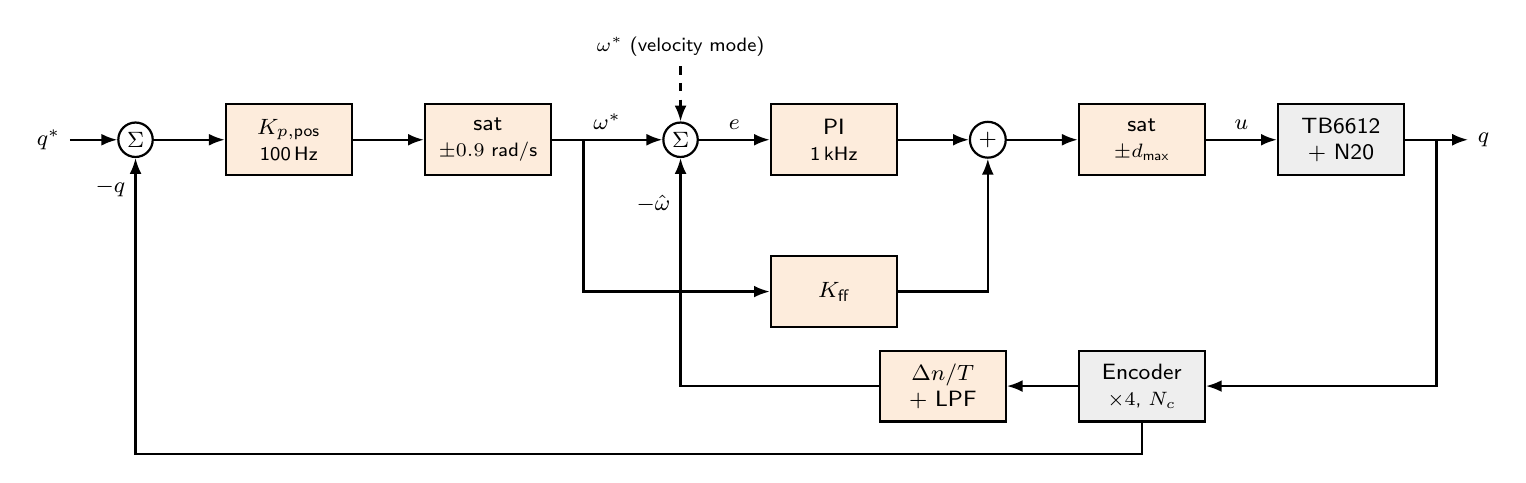
\begin{tikzpicture}[
  font=\sffamily\footnotesize, node distance=9mm,
  b/.style={draw, thick, minimum height=9mm, minimum width=16mm, align=center, fill=stmorange},
  s/.style={draw, thick, circle, inner sep=1.5pt},
  arr/.style={-{Latex[length=2mm]}, thick}
]
\node (in) {$q^*$};
\node[s, right=6mm of in] (s1) {$\Sigma$};
\node[b, right=of s1] (kp) {$K_{p,\text{pos}}$\\ \scriptsize 100\,Hz};
\node[b, right=of kp] (sat1) {sat\\ \scriptsize $\pm0.9$ rad/s};
\node[s, right=14mm of sat1] (s2) {$\Sigma$};
\node[b, right=of s2] (pi) {PI\\ \scriptsize 1\,kHz};
\node[s, right=of pi] (s3) {$+$};
\node[b, right=of s3] (sat2) {sat\\ \scriptsize $\pm d_\text{max}$};
\node[b, right=of sat2, fill=hwgray] (plant) {TB6612\\+ N20};
\node[right=8mm of plant] (out) {$q$};
\node[b, below=10mm of pi] (ff) {$K_\text{ff}$};
\node[b, below=22mm of sat2, fill=hwgray] (enc) {Encoder\\ \scriptsize $\times4$, $N_c$};
\node[b, left=of enc] (lpf) {$\Delta n/T$\\ + LPF};
\node[above=7mm of s2] (vin) {\scriptsize $\omega^*$ (velocity mode)};
\draw[arr] (in) -- (s1);
\draw[arr] (s1) -- (kp);
\draw[arr] (kp) -- (sat1);
\draw[arr] (sat1) -- node[above] {$\omega^*$} (s2);
\draw[arr, dashed] (vin) -- (s2);
\draw[arr] (s2) -- node[above] {$e$} (pi);
\draw[arr] (pi) -- (s3);
\draw[arr] (s3) -- (sat2);
\draw[arr] (sat2) -- node[above] {$u$} (plant);
\draw[arr] (plant) -- (out);
\draw[arr] ($(sat1.east)+(4mm,0)$) |- (ff);
\draw[arr] (ff) -| (s3);
\draw[arr] ($(plant.east)+(4mm,0)$) |- (enc);
\draw[arr] (enc) -- (lpf);
\draw[arr] (lpf) -| node[pos=0.9, left] {$-\hat\omega$} (s2);
\draw[arr] (enc.south) -- ++(0,-4mm) -| node[pos=0.95, left] {$-q$} (s1);
\end{tikzpicture}}
\caption{Cascaded controller run for each motor on the STM32. Wheels use velocity mode (the
dashed input); the inner pan/tilt gears use position mode.}
\label{pr3:fig:pid}
\end{figure}

\begin{table}[H]
\centering
\caption{Controller parameters (starting values, still to be tuned on the module).}
\label{pr3:tab:gains}
\small
\begin{tabular}{l c p{6.2cm}}
\toprule
Parameter & Value & Note \\
\midrule
$K_p$, $K_i$, $K_d$ (velocity) & 0.30, 1.50, 0 & duty per rad/s \\
$K_\text{ff}$ & 0.80 & slightly below $1/0.98$ so a stronger motor does not overshoot \\
$K_{p,\text{pos}}$, $K_{i,\text{pos}}$, $K_{d,\text{pos}}$ & 0.80, 0, 0 & kept low because the velocity signal is coarse \\
Position-loop velocity limit & \SI{0.9}{rad/s} & \\
Duty limit $d_\text{max}$ & 1.0 & full duty allowed \\
Velocity filter $\alpha$ & 0.10 & \\
\bottomrule
\end{tabular}
\end{table}

The starting gains were chosen by simulating the firmware's control code against a DC-motor
model built from the rated motor data (\SI{6}{V}, about \SI{0.98}{rad/s} at the spur gear at
full duty). They were checked on several variations of that model (faster, slower, weaker,
stronger, with a dead zone). They are a safe starting point, not final values.

\subsubsection{Interrupts and Data Flow}

The control tick (TIM10) has NVIC priority 1, and the USART2 and DMA interrupts have
priority 2, so the control loop always pre-empts frame parsing. USART2 receives into a
256-byte circular DMA buffer; the receive-to-idle callback passes only the new bytes to the
parser, including when the buffer wraps around. When a valid command arrives, the parser
copies all four modes and targets inside a short critical section, so the control loop never
uses a half-updated command. Targets that are NaN or infinite, and unknown modes, are replaced
by stop. Telemetry is sent from the main loop every \SI{20}{ms} with non-blocking DMA, on
USART2 and, when a PC is connected, on USB CDC. A UART error restarts reception from the main
loop. The LED shows the link state: a \SI{500}{ms} blink when commands arrive, \SI{250}{ms}
when the watchdog has tripped.

% ----------------------------------------------------------------------
\subsection{Safety and Fault Handling}
% ----------------------------------------------------------------------

\begin{table}[H]
\centering
\caption{Fault handling at each level.}
\label{pr3:tab:safety}
\small
\begin{tabularx}{\linewidth}{l l >{\raggedright\arraybackslash}X}
\toprule
Fault & Detected by & Reaction \\
\midrule
PC stops publishing \texttt{cmd\_vel}       & ESP32, 500\,ms timeout & Wheels commanded to \SI{0}{rad/s} (held, not coasting) \\
micro-ROS agent lost                      & ESP32, 3 failed pings  & Entities destroyed, reconnect loop; wheel timeout still applied \\
ESP32 stops sending (crash, cable)        & STM32, 200\,ms watchdog & All motors coast; flag in \texttt{MSG\_STATE}; fast LED blink \\
Corrupted or partial frame                & CRC-16, length check   & Frame dropped \\
NaN/Inf or unknown mode in a command      & ESP32 and STM32        & Command ignored (ESP32) or motor set to stop (STM32) \\
Pan/tilt command out of range             & ESP32 IK               & Clamped to $\pm\SI{0.5}{rad}$ \\
Stale feedback from the STM32 ($>$500\,ms)& ESP32                  & Feedback topics not published \\
Power-up, before any command              & both                   & All motors in stop; TB6612 kept in standby until the STM32 is set up \\
\bottomrule
\end{tabularx}
\end{table}

% ----------------------------------------------------------------------
\subsection{Bring-up and Test Results}
\label{pr3:sec:test}
% ----------------------------------------------------------------------

The system was brought up one level at a time, so each fault could be traced to one part:

\begin{enumerate}
  \item \textbf{STM32 alone, over USB-C.} The Python tool \texttt{test\_stm32.py} sends the same
        frames as the ESP32 over the USB virtual COM port. Its modes (\texttt{monitor},
        \texttt{duty}, \texttt{vel}, \texttt{pos}, \texttt{zero}) were used to run each motor, read all
        four encoders, and calibrate the direction and encoder signs in Table~\ref{pr3:tab:pins}.
        All four motors run under the STM32 firmware.
  \item \textbf{ESP32 $\rightarrow$ STM32 link.} A test build of the ESP32 firmware runs one
        motor at a time at 30\,\% duty for \SI{2}{s}, with a \SI{2}{s} stop in between. This
        confirmed the UART wiring and that index $i$ on the ESP32 moves the same physical motor
        as index $i$ on the STM32, which led to the renumbering in Table~\ref{pr3:tab:pins}.
  \item \textbf{Full chain through micro-ROS.} With the micro-ROS agent running on the PC,
        velocity commands (\texttt{Twist}) from a teleoperation node, sent on the module's
        wheel-command topic (Table~\ref{pr3:tab:topics}), drive the module. The wheel
        kinematics and the wheel direction sign work on the real module. Only the wheels were tested in this step; no
        pan/tilt commands were sent.
\end{enumerate}

\noindent\textbf{Result:} the wheel locomotion of the SMORES-EP style module works with the
architecture of Figure~\ref{fig:teleop-architecture}. The pan/tilt path (Eqs.~\eqref{pr3:eq:ptik}--\eqref{pr3:eq:ptfk},
position mode) is implemented in both firmwares but has \emph{not yet been tested} on the
module through ROS~2.

\subsubsection{Teleoperation Video}

A video of the module being teleoperated from the PC is available on Google Drive. Velocity
commands sent from ROS~2 drive the wheels through micro-ROS
(Figure~\ref{pr3:fig:video}).

\begin{figure}[H]
\centering
\begin{tabular}{c p{0.62\linewidth}}
\raisebox{-0.5\height}{\href{https://drive.google.com/file/d/1tHmvNSHuG8BPgNlsanB781ZCGBjsgjm0/view?usp=sharing}{\qrcode[nolink,height=2.8cm]{https://drive.google.com/file/d/1tHmvNSHuG8BPgNlsanB781ZCGBjsgjm0/view?usp=sharing}}} &
\raggedright Scan the QR code or open:\\[1mm]
\footnotesize\url{https://drive.google.com/file/d/1tHmvNSHuG8BPgNlsanB781ZCGBjsgjm0/view?usp=sharing}
\end{tabular}
\caption{Teleoperation video: the SMORES-EP style module driven by ROS~2 velocity commands through micro-ROS (wheel locomotion).}
\label{pr3:fig:video}
\end{figure}


% ----------------------------------------------------------------------
\subsection{Remaining Work}
% ----------------------------------------------------------------------

\begin{itemize}
  \item Tune the velocity and position gains on the module and record step responses
        (overshoot, settling time, steady-state error) for the Phase~A test plan (Section~\ref{sec:software-testing}).
  \item Test pan and tilt through ROS~2 (\texttt{head\_position\_controller/commands}); verify the direction signs ($K_t$, $K_p$) and widen the $\pm\SI{0.5}{rad}$
        limits after testing; add homing, since the encoders are incremental.
  \item Check the sign convention of the feedback topics against the commanded direction,
        and integrate \texttt{esp32/vel\_state} into an odometry estimate on the PC.
  \item Make the module namespace configurable (for example in \texttt{menuconfig}) so that
        several modules can run the same build.
  \item ESP32-C6 GPIO4 and GPIO5 are strapping pins. No problem has been seen so far, but if the
        ESP32 misbehaves at boot only while the STM32 is connected, the UART should move to
        other pins on the Phase~A main board.
  \item Carry the Table~\ref{pr3:tab:pins} pin map and the PC15 standby pin into the Phase~A
        main-board PCB.
\end{itemize}

\clearpage
% ================================================================
\section{Software Testing Plan (Phase A)}
\label{sec:software-testing}

\subsection{Objectives}

Verify the integrated software pipeline: AprilTag detection and robot ID via external camera $\rightarrow$ real-time pose estimation $\rightarrow$ PID motor control $\rightarrow$ path planning and execution for MSRR configurations.

\subsection{Setup}

MSRR robot in a controlled indoor environment with an external camera, AprilTags for ID and pose reference, and a computing system running perception, localisation, planning, and control.

\subsection{Goal Configurations}

Snake, Car, DoubleDriver, L-shape.

\subsection{Evaluation Metrics}

\begin{itemize}
\item \textbf{Detection rate} --- \% frames with correct AprilTag ID.
\item \textbf{Position / orientation error} --- estimated vs.\ reference pose.
\item \textbf{Tracking error} --- desired vs.\ actual position and heading during path following.
\item \textbf{Control response} --- PID overshoot and steady-state error.
\item \textbf{Processing rate} --- perception + control update frequency.
\end{itemize}

\subsection{Acceptance Criteria}

Reliable tag detection, acceptable localisation and tracking error for real-time control, stable PID behaviour without excessive oscillation, and continuous operation without critical failures. Specific numerical thresholds to be defined based on system requirements.

\subsection{Navigation and Avoidance Plan}
\label{sec:nav-plan}

This plan covers the \textbf{simulation stage} only.

Reconfiguration planning follows the parallel self-assembly method of Liu et al.\ \cite{liu2023}, which was developed for SMORES-EP, the platform on which our module is based. The method consists of three stages: assigning each physical module to a position in the target configuration, determining the order in which modules connect, and driving each module into place to dock. Coordinated motion of multiple modules without collisions is handled by the prioritised route planner of Binder et al.\ \cite{binder2019,binder2017}.

\subsubsection{Planning Stages}

A target configuration is represented as a tree in which each edge specifies the two connecting faces: T (top, the pan face), B (bottom), or L/R (the left and right wheel faces) \cite{liu2017}. The planar pose of each module is denoted $[x, y, \theta]$.

\begin{enumerate}[topsep=2pt,itemsep=2pt,parsep=0pt,leftmargin=1.5em]
\item \textbf{Task assignment.} A root module is selected at the centre of the target configuration, and the pose of every target position is expressed relative to it. Likewise, the physical module closest to the centroid of the group is selected as the physical root, and all physical poses are expressed relative to it. The cost of assigning a module to a target position is the distance between their relative positions, and the Hungarian algorithm \cite{kuhn1955,munkres1957} finds the assignment with the minimum total distance. The output is a goal pose for every module.
\item \textbf{Assembly sequence.} The configuration is assembled outward from the root, one tree layer at a time. Each module in a layer connects to a module that is already in place, so all modules in the same layer can move in parallel. Each connection is written $(m, c, \tilde{m}, \tilde{c}')$, meaning module $m$ connects its face $c$ to face $\tilde{c}'$ of module $\tilde{m}$. When several modules connect directly to the root, L/R connections are performed before T/B connections.
\item \textbf{Docking.} Each module navigates to the vicinity of its parent, aligns with the target face, and approaches it (Sections~\ref{sec:nav-avoid} and~\ref{sec:nav-dock}).
\end{enumerate}

\subsubsection{Navigation and Collision Avoidance}
\label{sec:nav-avoid}

The workspace is discretised into a \SI{10}{cm} grid \cite{liu2023}, and routes are planned over its cells. Each module is modelled as a differential-drive robot, with forward velocity $v$ and angular velocity $\omega$ produced by the two wheels:
\begin{equation}
\begin{bmatrix} \dot{x} \\ \dot{y} \\ \dot{\theta} \end{bmatrix} =
\begin{bmatrix} \cos\theta & 0 \\ \sin\theta & 0 \\ 0 & 1 \end{bmatrix}
\begin{bmatrix} v \\ \omega \end{bmatrix}.
\end{equation}

Each module first navigates to a waypoint one grid cell away from its docking pose.

\begin{itemize}
\item \textbf{Prioritised planning.} Modules are assigned a priority order and planned sequentially. Each route is found with a time-aware A* search, in which a cell occupied by a previously planned module at a given time is treated as blocked. Waiting in place is permitted, and cell reservations overlap slightly in time so that two modules exchanging cells are detected as a collision.
\item \textbf{Conflict resolution.} When a route is blocked, the planner applies five strategies in order: backtracking and waiting, yielding into a side branch at a crossing, yielding from the start cell, vacating the goal cell for a higher-priority module, and pushing the waiting position further along the route.
\item \textbf{Rescheduling.} If no route is found, the maximum speed of the module causing the most conflicts is reduced. If this is insufficient, the priorities of the two most conflicting modules are swapped and planning is repeated.
\item \textbf{Execution.} Each route segment carries a precondition of the form ``module $x$ has passed step $n$''. Each module tracks its route with a PID controller and publishes its current step, allowing the other modules to check their preconditions.
\end{itemize}

\subsubsection{Alignment and Approach}
\label{sec:nav-dock}

On reaching its waypoint, the module aligns with the target face. Let $(x', y', \theta')$ denote the module's pose error relative to its docking pose. For L/R connections, the controller drives $x'$ and $\theta'$ to zero; for T/B connections, it drives $y'$ and $\theta'$ to zero. The module then moves straight forward until it contacts its parent. As the simulation does not model the EP magnets, a dock is considered successful when the modules are in contact and the residual error is within a set tolerance. On the physical system, L/R connections require a helper module to lift the moving module \cite{liu2023}; this connection type may therefore be excluded to reduce project complexity.

\subsubsection{Test Procedure}

\textbf{Setup.} Gazebo Fortress spawns $N$ modules in a row, each with its own differential-drive controller. Ground-truth poses from the simulator replace AprilTag localisation, and the linear speed is limited to \SI{0.049}{m/s} to match the physical motors.

\textbf{Tests.} Tests are performed in increasing order of complexity: the planner in isolation (verifying that the assignment is optimal against an exhaustive search and that the assembly sequence is correct); single-module navigation to a goal; two-module conflict scenarios (head-on, crossing paths, an occupied goal, and a narrow passage); alignment and approach; and finally assembly of the goal configurations listed above.

\textbf{Metrics.} Success rate, number of collisions (centre distance below one module width), planning time, total completion time, path-tracking error, and final alignment error.

\textbf{Initial test case.} The first planner test uses three modules connected side by side ($v_3$--$v_2$--$v_1$, joined L to R), starting from the default simulation spawn positions. The expected output is shown in Table~\ref{tab:nav-n1}: the middle module becomes the root, and both outer modules connect to it in parallel. As this configuration uses only L/R connections, it would be affected if that connection type is excluded.

\begin{table}[!htbp]
\centering
\caption{Expected planner output for three modules side by side, starting at $y = -0.3, 0, 0.3$\,m.}
\label{tab:nav-n1}
\small
\begin{tabular}{@{}lll@{}}
\toprule
\textbf{Target position} & \textbf{Assigned module} & \textbf{Goal pose $(x, y, \theta)$} \\
\midrule
$v_2$ (root) & module\_2 (root) & $(0,\ 0,\ 0^\circ)$ \\
$v_1$ & module\_3 & $(0,\ +0.1,\ 0^\circ)$ \\
$v_3$ & module\_1 & $(0,\ -0.1,\ 0^\circ)$ \\
\midrule
\multicolumn{3}{@{}l}{Parallel connections: (module\_3, R, module\_2, L), (module\_1, L, module\_2, R)} \\
\bottomrule
\end{tabular}
\end{table}

\clearpage
% ================================================================
\section{Preparation for Phase B: EP Magnet}
\label{sec:phase-b-magnet}

The docking system uses an Electro-Permanent Magnet (EPM) connector based on SMORES-EP \cite{tosun2016}. Each EP unit pairs an AlNiCo~5 magnet (low coercivity, switchable) with an NdFeB magnet (high coercivity, fixed) between steel pole pieces, wound with a copper coil. 

\begin{figure}[!htbp]
    \centering
    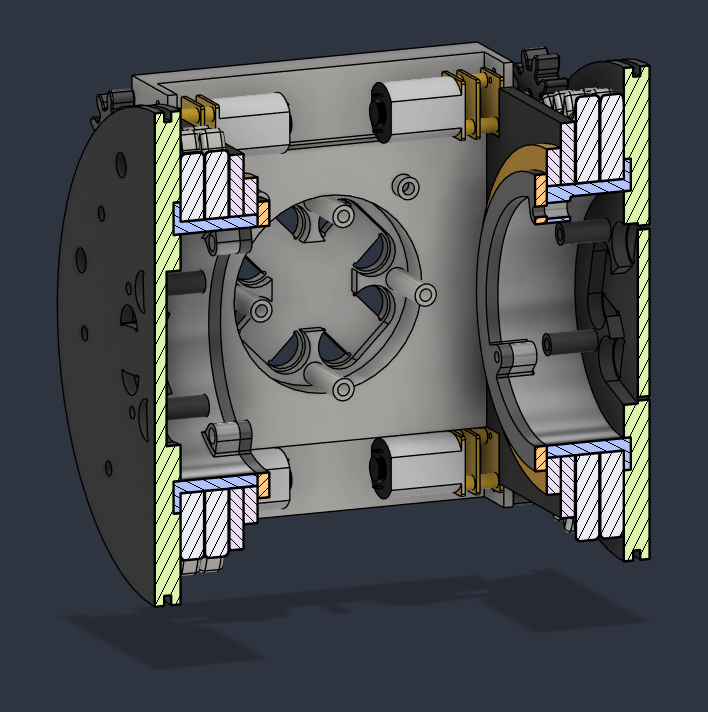
\includegraphics[width=0.6\textwidth]{../image/inside_rectangular_magnet_housing.png}
    \caption{Interior view of the rectangular magnet housing.}
    \label{fig:cad-magnet-housing}
\end{figure}

\textbf{Operating principle:} A current pulse through the coil reverses AlNiCo~5 magnetisation while NdFeB stays fixed. Fields aligned $\rightarrow$ \textbf{ON} (attract); fields opposed $\rightarrow$ \textbf{OFF} (release). No power needed to hold either state.

The original EP-Face connector was developed for a significantly smaller robotic framework. To accommodate our larger target module dimensions of $100\times100\times100$~mm, we had to redesign the baseline architecture. Furthermore, due to the strict standard sizes of magnets available in the Thai market, we altered the core magnet dimensions and completely recalculated the system's electrical and mechanical properties to ensure compatibility and structural integrity.

\subsection{System Architecture and Parametric Scaling}
To fulfill the increased load requirements of our larger module, we scaled several primary parameters from the original reference design:
\begin{itemize}
    \item \textbf{Magnet Dimensions:} The original design utilized $4.76 \times 9.53$~mm magnets. We increased this to $5 \times 15$~mm for both the high-coercivity NdFeB N52 and low-coercivity AlNiCo 5 cylinder magnets.
    \item \textbf{Module Integration:} The original magnets were arranged in a $\varnothing 42$~mm ring. To fit our larger module face, the 4 EP magnets are now arranged within a $\varnothing 50$~mm ring. 
    \item \textbf{Physical Footprint:} The overall length of our EP magnet assembly is $25.6$~mm. The pole piece body has a diameter of $10.6$~mm, while the protruding contact foot has a diameter of $9.6$~mm. The total height of the pole piece is $11.8$~mm, with the contact plane extending $0.5$~mm outward from the module face.
    \item \textbf{Weight:} The increased dimensions raise the weight from $10.6$~g to $19.4$~g per EP magnet.
\end{itemize}

\begin{figure}[H]
    \centering
    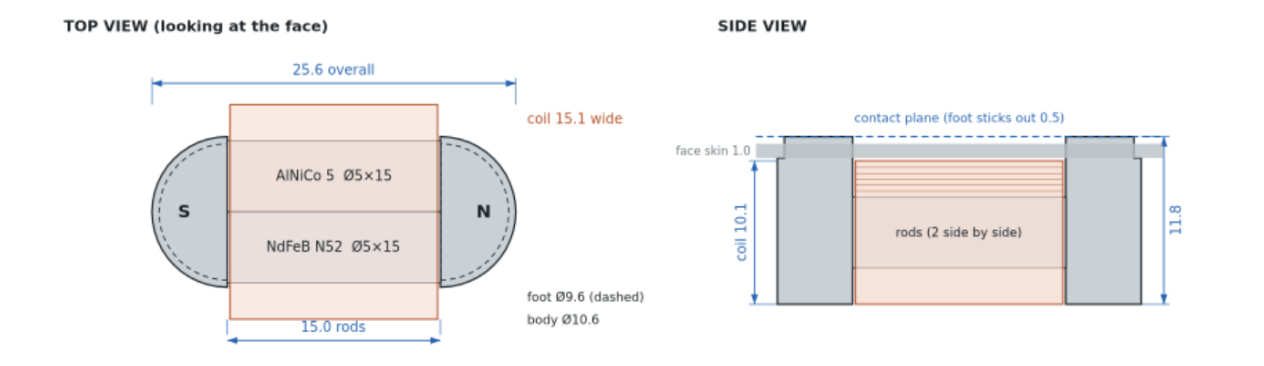
\includegraphics[width=0.9\textwidth]{../image/ep_magnet_diagram.png}
    \caption{Top and side view dimensions of the redesigned $5 \times 15$~mm EP Magnet.}
    \label{fig:ep_diagram}
\end{figure}

\begin{figure}[H]
    \centering
    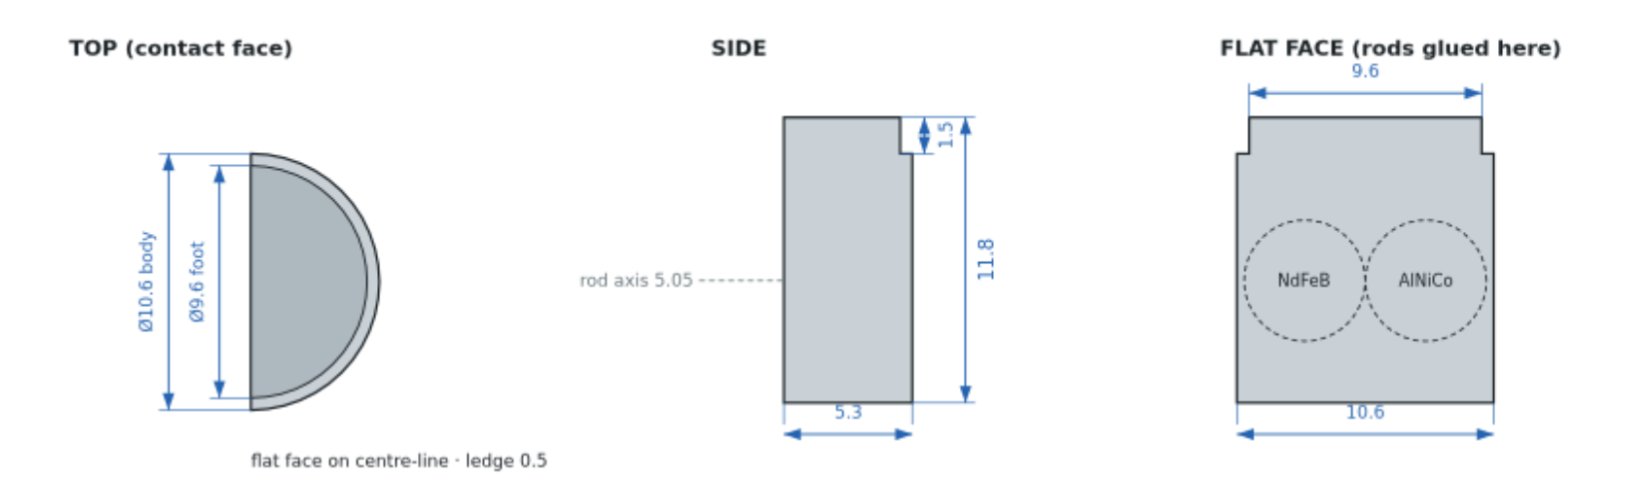
\includegraphics[width=0.9\textwidth]{../image/pole_piece_drawing.png}
    \caption{Detailed mechanical drawing of the low-carbon steel pole piece, illustrating the body and protruding contact foot.}
    \label{fig:pole_piece}
\end{figure}

\subsection{Coil Design and Electrical Specifications}
The coil winding was strictly recalculated to maximize the magnetic field without exceeding the physical constraints of the $11.8$~mm pole pieces. 
\begin{itemize}
    \item \textbf{Wire Selection:} We transitioned from the original AWG 30 wire to SWG 28 double-coated enameled copper wire.
    \item \textbf{Winding Configuration:} The coil consists of exactly 210 turns. This is distributed precisely into 6 complete layers, with each layer containing exactly 35 turns.
    \item \textbf{Wire Length:} Due to the capsule shape of the coil wrapped around the two magnet bars, the perimeter expands with each subsequent layer. The first layer has a perimeter of $27.3$~mm, expanding to $40.4$~mm by the sixth layer. The total length of copper wire required per EP magnet is $7115.3$~mm.
\end{itemize}

\begin{figure}[H]
    \centering
    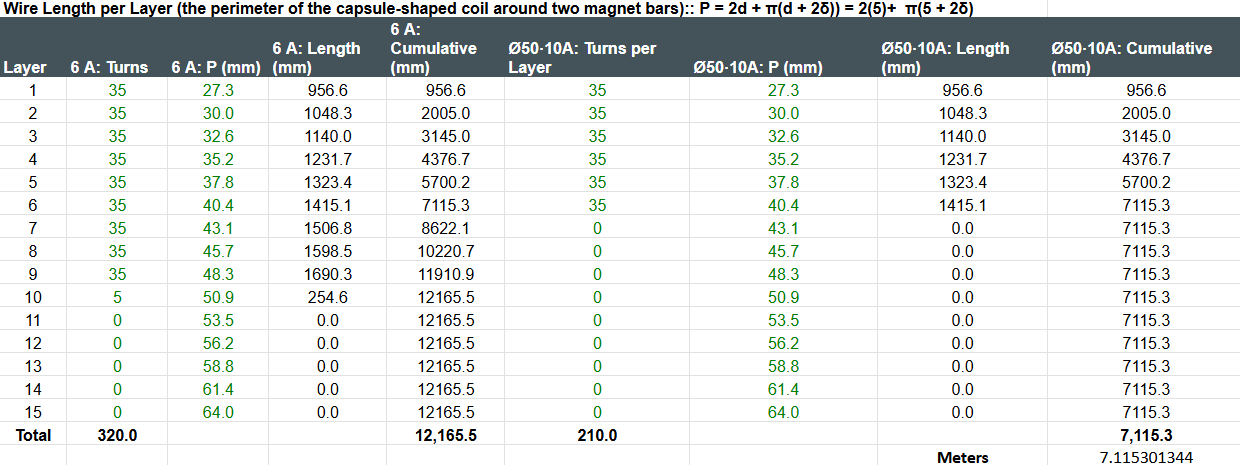
\includegraphics[width=\textwidth]{../image/image_701f62.png}
    \caption{Wire length calculations per layer demonstrating the 6-layer, 210-turn configuration.}
    \label{fig:wire_length}
\end{figure}

\subsubsection{Mathematical Modeling and Formula Derivations}
To ensure the larger system meets the required strength characteristics, the following mathematical formulas were applied to derive our final design parameters:
\begin{itemize}
    \item \textbf{Magnet Area and Total Flux:} The cross-sectional area of the cylindrical magnet rod ($A_{rod}$) is calculated first. $$A_{rod} = \frac{\pi d^2}{4} = \frac{\pi (5)^2}{4} = 19.63 \text{ mm}^2$$ The total magnetic flux ($\Phi$) combines the remnant magnetization of both the NdFeB and AlNiCo magnets. $$\Phi = A_{rod}(Br_{Nd} + Br_{Al}) = 19.63(1.455 + 1.265) = 53.4 \text{ T}\cdot\text{mm}^2$$
    \item \textbf{Minimum Foot Area:} To prevent magnetic saturation within the low-carbon steel, we assume a saturation point ($B_{sat}$) of $1.5$~T to find the minimum required area ($A_{min}$). $$A_{min} = \frac{\Phi}{B_{sat}} = \frac{53.4}{1.5} = 35.6 \text{ mm}^2$$ This minimum area dictates that the minimum foot diameter ($D_{min}$) must be $9.52$~mm. $$D_{min} = \sqrt{\frac{8A_{min}}{\pi}} = 9.52 \text{ mm}$$
    \item \textbf{Magnetic Flux Density in Foot:} By utilizing our selected foot diameter of $9.6$~mm, the actual surface area is $36.2~\text{mm}^2$. This yields an actual magnetic flux density ($B$) at the contact surface. $$B = \frac{\Phi}{A_{foot}} = \frac{53.4}{36.2} = 1.48 \text{ T}$$
    \item \textbf{Holding Force Calibration:} Magnetic holding force is proportional to $B^2 A / (2\mu_0)$. We scale the force directly from the reference paper's maximum baseline force of $90$~N ($F_{paper}$). The scaling multiplier $1.078$ represents the proportional increase in strength due to our larger contact area and stronger flux. The term $f(H)$ acts as a compensation factor for polarization reversal percentage. $$F = F_{paper} \times \frac{(B^2 A)}{(B^2 A)_{paper}} \times f(H) = 90 \text{ N} \times 1.078 \times f(H)$$
    \item \textbf{Mean Length of Turn (MLT):} Because the coil is wrapped around two parallel magnet bars, the winding forms a capsule shape. The length for each coil layer $j$ includes the two straight sides ($2d$) and the two curved ends ($\pi(d + 2\delta_j)$), where $\delta_j$ represents thickness increment per layer. $$MLT_j = 2d + \pi(d + 2\delta_j)$$
    \item \textbf{Coil Resistance:} The total resistance is computed using the resistivity of copper ($\rho$) and the sum of the wire lengths across all layers. $$R = \frac{\rho \sum (N_j \cdot MLT_j)}{A_{wire}} = \frac{1.724 \times 10^{-8} \times 7.12}{0.111 \times 10^{-6}} = 1.105~\Omega$$
    \item \textbf{Current and Magnetic Field (H):} Operating at $12$~V, we estimate an external resistance ($R_{ext}$) of $0.15~\Omega$ for the wiring and MOSFET components. $$I = \frac{V}{(R + R_{ext})} = \frac{12}{1.255} = 9.56 \text{ A}$$ This current generates an applied field capable of fully reversing the AlNiCo 5 polarity. $$H = \frac{NI}{L} = \frac{2008}{0.015} = 134 \text{ kA/m}$$
    \item \textbf{Switching Energy:} The total energy consumed to switch states is calculated by multiplying voltage, current, duration per pulse ($4$~ms), and number of pulses ($3$). $$E = V \cdot I \cdot t \cdot 3 = 12 \times 9.56 \times 0.004 \times 3 = 1.38 \text{ J}$$
\end{itemize}

\subsubsection{Performance Metrics}
The new coil and magnet configuration yields significant performance improvements over the original paper:
\begin{itemize}
    \item \textbf{Electrical Resistance:} Our configuration yields a coil resistance of $1.105~\Omega$, compared to the original $2.08~\Omega$.
    \item \textbf{Magnetic Field and Current:} Driven at $12$~V, the system draws $9.56$~A, generating an operating field of $134$~kA/m. At a peak battery voltage of $12.6$~V, the current reaches $10.04$~A, generating a field of $141$~kA/m. The original design achieved $\approx 6$~A and $121$~kA/m.
    \item \textbf{Holding Force:} The contact surface area is $36.2~\text{mm}^2$ with a magnetic flux density of $\approx 1.48$~T. This results in an expected holding force of $\approx 32$~N per EP pair, yielding a total face holding force of $\approx 97$~N. The original paper averaged $28.3$~N per pair and $88.4$~N per face.
    \item \textbf{Switching Energy:} The required switching energy per face is $\approx 5.5$~J, utilizing three $4$~ms pulses per EP. The original system required $2.5$~J using $3$~ms pulses.
\end{itemize}

\subsection{Current Progress and Procurement Challenges}
\label{sec:ep-progress}
% ======================================================================

The EP magnet follows the design above: an AlNiCo~5 and an NdFeB~N52 rod, both
$\varnothing5\times\SI{15}{mm}$, between two low-carbon steel pole pieces, wound with 210
turns of SWG~28 wire (6 layers $\times$ 35 turns). This period focused on the two
procurement and fabrication problems reported in Progress Report~2: sourcing the AlNiCo~5 magnets and making the pole pieces.

\subsubsection{Procurement}

The AlNiCo~5 magnets, which were the hardest part to source, have now been ordered from a
supplier in China. With this order, all the materials for the first EP magnets have been
purchased or ordered (Table~\ref{pr3:tab:epbom}). The coil driver (half-bridges rated for at
least \SI{10}{A}) has not been bought yet.

\begin{table}[H]
\centering
\caption{EP magnet material status.}
\label{pr3:tab:epbom}
\small
\begin{tabularx}{\linewidth}{l >{\raggedright\arraybackslash}X l}
\toprule
Part & Specification & Status \\
\midrule
AlNiCo 5 rod            & $\varnothing5\times\SI{15}{mm}$ & Ordered from China \\
NdFeB N52 rod           & $\varnothing5\times\SI{15}{mm}$, Ni-Cu-Ni coating & Purchased \\
Magnet wire             & SWG 28, double-coated enamel, \SI{220}{\celsius} class, \SI{98.4}{m} (\SI{0.1}{kg}) & Purchased \\
Pole-piece stock        & SS400 steel rod, $\varnothing\SI{12}{mm}$ & In hand; machine access arranged \\
Kapton tape, CA glue gel& \SI{15}{mm} tape; high-viscosity gel & Purchased \\
Coil driver             & Half-bridge, $\geq\SI{10}{A}$ per channel & Not yet ordered \\
\bottomrule
\end{tabularx}
\end{table}

The wire on hand is enough for the first prototype: at \SI{7.1}{m} per EP magnet
(coil design above), the 8-EP prototype needs about \SI{57}{m} of the \SI{98.4}{m} reel.

\subsubsection{Pole-Piece Fabrication}

External machine shops and wire-cut services would not take the pole pieces because they are
too small. The team will therefore make them in-house from a $\varnothing\SI{12}{mm}$ SS400
steel rod. Use of the milling and cutting machines at the Hans Building has been arranged,
and the team is ready to start milling and cutting the rod to the pole-piece geometry of
Figure~\ref{fig:pole_piece}: a
\SI{10.6}{mm} body, a \SI{9.6}{mm} semicircular contact foot, \SI{11.8}{mm} total height, with
the contact plane standing \SI{0.5}{mm} out from the module face.

SS400 is a general structural steel (JIS G3101). The standard specifies its strength rather
than its carbon content, but the grade is normally a low-carbon steel, so it is expected to
behave like the low-carbon steel assumed in the flux calculation above; this will be confirmed in the first
holding-force test. The \SI{12}{mm} rod leaves about \SI{0.7}{mm} of stock on each side of the
\SI{10.6}{mm} body for machining.

The foot is the dimension that needs the most care. From the flux calculation above, the minimum foot diameter that
keeps the steel below the assumed saturation of \SI{1.5}{T} is \SI{9.52}{mm}, against
the \SI{9.6}{mm} design. A foot machined more than about \SI{0.08}{mm} undersize would
therefore push the steel into saturation and reduce the holding force. The contact faces also
need to be flat and level with each other, since any air gap between two connected faces
reduces the holding force.

\subsubsection{Next Steps}

\begin{enumerate}
  \item Mill and cut the pole pieces from the SS400 rod and measure the foot diameters and heights.
  \item Wind the coils (210 turns, 6 $\times$ 35) and check each coil's resistance against the
        calculated \SI{1.105}{\ohm}.
  \item Assemble the first EP magnets when the AlNiCo~5 rods arrive.
  \item Select and order the $\geq\SI{10}{A}$ half-bridge driver, then run the first
        switching and holding-force tests (EP Face 1st Test in the schedule).
\end{enumerate}

% 

\renewcommand{\refname}{Additional References}
\begin{thebibliography}{9}

\bibitem{tosun2016}
Tosun, T., Davey, J., Liu, C., \& Yim, M. (2016). Design and characterization
of the EP-Face connector. In \textit{IEEE/RSJ International Conference on
Intelligent Robots and Systems (IROS)} (pp.\ 45--51).

\bibitem{liu2023}
Liu, C., Lin, Q., Kim, H., \& Yim, M. (2023). SMORES-EP, a modular robot with
parallel self-assembly. \textit{Autonomous Robots}, 47, 211--228.
doi:10.1007/s10514-022-10078-1.

\bibitem{liu2017}
Liu, C., \& Yim, M. (2019). Configuration recognition with distributed
information for modular robots. In \textit{Robotics Research (ISRR 2017)},
Springer Proceedings in Advanced Robotics, vol.\ 10 (pp.\ 967--983).

\bibitem{binder2019}
Binder, B., Beck, F., K\"onig, F., \& Bader, M. (2019). Multi robot route
planning (MRRP): Extended spatial-temporal prioritized planning. In
\textit{IEEE/RSJ International Conference on Intelligent Robots and Systems
(IROS)} (pp.\ 4133--4139).

\bibitem{binder2017}
Binder, B. (2017). \textit{Spatio-temporal prioritized planning}. Master's
thesis, TU Wien.

\bibitem{kuhn1955}
Kuhn, H.\ W. (1955). The Hungarian method for the assignment problem.
\textit{Naval Research Logistics Quarterly}, 2(1--2), 83--97.

\bibitem{munkres1957}
Munkres, J. (1957). Algorithms for the assignment and transportation problems.
\textit{Journal of the SIAM}, 5(1), 32--38.

\bibitem{microros}
micro-ROS project. \textit{micro-ROS: ROS~2 for microcontrollers}.
\url{https://micro.ros.org}

\end{thebibliography}

\end{document}